\PassOptionsToPackage{unicode=true}{hyperref} % options for packages loaded elsewhere
\PassOptionsToPackage{hyphens}{url}
%
\documentclass[]{book}
\usepackage{lmodern}
\usepackage{amssymb,amsmath}
\usepackage{ifxetex,ifluatex}
\usepackage{fixltx2e} % provides \textsubscript
\ifnum 0\ifxetex 1\fi\ifluatex 1\fi=0 % if pdftex
  \usepackage[T1]{fontenc}
  \usepackage[utf8]{inputenc}
  \usepackage{textcomp} % provides euro and other symbols
\else % if luatex or xelatex
  \usepackage{unicode-math}
  \defaultfontfeatures{Ligatures=TeX,Scale=MatchLowercase}
\fi
% use upquote if available, for straight quotes in verbatim environments
\IfFileExists{upquote.sty}{\usepackage{upquote}}{}
% use microtype if available
\IfFileExists{microtype.sty}{%
\usepackage[]{microtype}
\UseMicrotypeSet[protrusion]{basicmath} % disable protrusion for tt fonts
}{}
\IfFileExists{parskip.sty}{%
\usepackage{parskip}
}{% else
\setlength{\parindent}{0pt}
\setlength{\parskip}{6pt plus 2pt minus 1pt}
}
\usepackage{hyperref}
\hypersetup{
            pdftitle={TRES Tidyverse Tutorial},
            pdfauthor={Raphael, Pratik and Theo},
            pdfborder={0 0 0},
            breaklinks=true}
\urlstyle{same}  % don't use monospace font for urls
\usepackage{color}
\usepackage{fancyvrb}
\newcommand{\VerbBar}{|}
\newcommand{\VERB}{\Verb[commandchars=\\\{\}]}
\DefineVerbatimEnvironment{Highlighting}{Verbatim}{commandchars=\\\{\}}
% Add ',fontsize=\small' for more characters per line
\newenvironment{Shaded}{}{}
\newcommand{\AlertTok}[1]{\textcolor[rgb]{1.00,0.00,0.00}{\textbf{#1}}}
\newcommand{\AnnotationTok}[1]{\textcolor[rgb]{0.38,0.63,0.69}{\textbf{\textit{#1}}}}
\newcommand{\AttributeTok}[1]{\textcolor[rgb]{0.49,0.56,0.16}{#1}}
\newcommand{\BaseNTok}[1]{\textcolor[rgb]{0.25,0.63,0.44}{#1}}
\newcommand{\BuiltInTok}[1]{#1}
\newcommand{\CharTok}[1]{\textcolor[rgb]{0.25,0.44,0.63}{#1}}
\newcommand{\CommentTok}[1]{\textcolor[rgb]{0.38,0.63,0.69}{\textit{#1}}}
\newcommand{\CommentVarTok}[1]{\textcolor[rgb]{0.38,0.63,0.69}{\textbf{\textit{#1}}}}
\newcommand{\ConstantTok}[1]{\textcolor[rgb]{0.53,0.00,0.00}{#1}}
\newcommand{\ControlFlowTok}[1]{\textcolor[rgb]{0.00,0.44,0.13}{\textbf{#1}}}
\newcommand{\DataTypeTok}[1]{\textcolor[rgb]{0.56,0.13,0.00}{#1}}
\newcommand{\DecValTok}[1]{\textcolor[rgb]{0.25,0.63,0.44}{#1}}
\newcommand{\DocumentationTok}[1]{\textcolor[rgb]{0.73,0.13,0.13}{\textit{#1}}}
\newcommand{\ErrorTok}[1]{\textcolor[rgb]{1.00,0.00,0.00}{\textbf{#1}}}
\newcommand{\ExtensionTok}[1]{#1}
\newcommand{\FloatTok}[1]{\textcolor[rgb]{0.25,0.63,0.44}{#1}}
\newcommand{\FunctionTok}[1]{\textcolor[rgb]{0.02,0.16,0.49}{#1}}
\newcommand{\ImportTok}[1]{#1}
\newcommand{\InformationTok}[1]{\textcolor[rgb]{0.38,0.63,0.69}{\textbf{\textit{#1}}}}
\newcommand{\KeywordTok}[1]{\textcolor[rgb]{0.00,0.44,0.13}{\textbf{#1}}}
\newcommand{\NormalTok}[1]{#1}
\newcommand{\OperatorTok}[1]{\textcolor[rgb]{0.40,0.40,0.40}{#1}}
\newcommand{\OtherTok}[1]{\textcolor[rgb]{0.00,0.44,0.13}{#1}}
\newcommand{\PreprocessorTok}[1]{\textcolor[rgb]{0.74,0.48,0.00}{#1}}
\newcommand{\RegionMarkerTok}[1]{#1}
\newcommand{\SpecialCharTok}[1]{\textcolor[rgb]{0.25,0.44,0.63}{#1}}
\newcommand{\SpecialStringTok}[1]{\textcolor[rgb]{0.73,0.40,0.53}{#1}}
\newcommand{\StringTok}[1]{\textcolor[rgb]{0.25,0.44,0.63}{#1}}
\newcommand{\VariableTok}[1]{\textcolor[rgb]{0.10,0.09,0.49}{#1}}
\newcommand{\VerbatimStringTok}[1]{\textcolor[rgb]{0.25,0.44,0.63}{#1}}
\newcommand{\WarningTok}[1]{\textcolor[rgb]{0.38,0.63,0.69}{\textbf{\textit{#1}}}}
\usepackage{longtable,booktabs}
% Fix footnotes in tables (requires footnote package)
\IfFileExists{footnote.sty}{\usepackage{footnote}\makesavenoteenv{longtable}}{}
\usepackage{graphicx,grffile}
\makeatletter
\def\maxwidth{\ifdim\Gin@nat@width>\linewidth\linewidth\else\Gin@nat@width\fi}
\def\maxheight{\ifdim\Gin@nat@height>\textheight\textheight\else\Gin@nat@height\fi}
\makeatother
% Scale images if necessary, so that they will not overflow the page
% margins by default, and it is still possible to overwrite the defaults
% using explicit options in \includegraphics[width, height, ...]{}
\setkeys{Gin}{width=\maxwidth,height=\maxheight,keepaspectratio}
\setlength{\emergencystretch}{3em}  % prevent overfull lines
\providecommand{\tightlist}{%
  \setlength{\itemsep}{0pt}\setlength{\parskip}{0pt}}
\setcounter{secnumdepth}{5}
% Redefines (sub)paragraphs to behave more like sections
\ifx\paragraph\undefined\else
\let\oldparagraph\paragraph
\renewcommand{\paragraph}[1]{\oldparagraph{#1}\mbox{}}
\fi
\ifx\subparagraph\undefined\else
\let\oldsubparagraph\subparagraph
\renewcommand{\subparagraph}[1]{\oldsubparagraph{#1}\mbox{}}
\fi

% set default figure placement to htbp
\makeatletter
\def\fps@figure{htbp}
\makeatother


\usepackage{fontspec}
% use nice fonts if available else use boring defaults
\IfFontExistsTF{IBM Plex Serif}{\setmainfont[]{IBM Plex Serif}}{} 
\IfFontExistsTF{Hack}{\setmonofont[]{Hack}}{}

\usepackage{lineno}

\usepackage{color}
\usepackage{framed}
\setlength{\fboxsep}{.8em}

\newenvironment{blackbox}{
  \definecolor{shadecolor}{rgb}{0.9, 0.9, 0.9}  % black
  \color{black}
  \begin{shaded}}
 {\end{shaded}}

% create infobox environment
\newenvironment{infobox}[1]
  {
  \begin{itemize}
  \renewcommand{\labelitemi}{
    \raisebox{-.7\height}[0pt][0pt]{
      {\setkeys{Gin}{width=3em,keepaspectratio}
        % \includegraphics{images/#1}
        }
    }
  }
  \setlength{\fboxsep}{1em}
  \begin{blackbox}
  \item
  }
  {
  \end{blackbox}
  \end{itemize}
  }

\title{TRES Tidyverse Tutorial}
\author{Raphael, Pratik and Theo}
\date{2020-06-14}

\begin{document}
\maketitle


\linenumbers

{
\setcounter{tocdepth}{1}
\tableofcontents
}
\hypertarget{outline}{%
\chapter*{Outline}\label{outline}}
\addcontentsline{toc}{chapter}{Outline}

This is the readable version of the TRES \href{https://www.tidyverse.org/}{tidyverse} tutorial. A convenient PDF version can be downloaded by clicking the PDF document icon in the header bar.

\hypertarget{about}{%
\section*{About}\label{about}}
\addcontentsline{toc}{section}{About}

The TRES tidyverse tutorial is an online workshop on how to use the tidyverse, a set of packages in the R computing language designed at making data handling and plotting easier.

This tutorial will take the form of a one hour per week video stream via Google Meet, every Friday morning at 10.00 (Groningen time) starting from the 29th of May, 2020 and lasting for a couple of weeks (depending on the number of topics we want to cover, but there should be at least 5).

\textbf{PhD students from outside our department are welcome to attend.}

\hypertarget{schedule}{%
\section*{Schedule}\label{schedule}}
\addcontentsline{toc}{section}{Schedule}

\begin{longtable}[]{@{}llll@{}}
\toprule
Topic & Package & Instructor & Date*\tabularnewline
\midrule
\endhead
Reading data and string manipulation & \href{https://readr.tidyverse.org/}{readr}, \href{https://stringr.tidyverse.org/}{stringr}, \href{https://github.com/tidyverse/glue}{glue} & Pratik & 29/05/20\tabularnewline
Data and reshaping & \href{https://tibble.tidyverse.org/}{tibble}, \href{https://tidyr.tidyverse.org/}{tidyr} & Raphael & 05/06/20\tabularnewline
Manipulating data & \href{https://dplyr.tidyverse.org/}{dplyr} & Theo & 12/06/20\tabularnewline
Working with lists and iteration & \href{https://purrr.tidyverse.org/}{purrr} & Pratik & 19/06/20\tabularnewline
Plotting & \href{https://ggplot2.tidyverse.org/}{ggplot2} & Raphael & 26/06/20\tabularnewline
Regular expressions & \href{https://stat.ethz.ch/R-manual/R-devel/library/base/html/regex.html}{regex} & Richel & 03/07/20\tabularnewline
Programming with the tidyverse & \href{https://rlang.r-lib.org/}{rlang} & Pratik & 10/07/20\tabularnewline
\bottomrule
\end{longtable}

\hypertarget{possible-extras}{%
\section*{Possible extras}\label{possible-extras}}
\addcontentsline{toc}{section}{Possible extras}

\begin{itemize}
\tightlist
\item
  Reproducibility and package-making (with e.g.~\href{https://usethis.r-lib.org/}{usethis})\\
\item
  Embedding C++ code with \href{http://adv-r.had.co.nz/Rcpp.html}{Rcpp}
\end{itemize}

\hypertarget{join}{%
\section*{Join}\label{join}}
\addcontentsline{toc}{section}{Join}

Join the Slack \href{https://join.slack.com/t/trestidytorial/shared_invite/zt-ejgr3tow-3zisGwPg1JDeTJD33DWb2A}{by clicking this link (Slack account required)}.

*Tentative dates.

\hypertarget{reading-files-and-string-manipulation}{%
\chapter{Reading files and string manipulation}\label{reading-files-and-string-manipulation}}


\includegraphics{opening-image.png}

Load the packages for the day.

\begin{Shaded}
\begin{Highlighting}[]
\KeywordTok{library}\NormalTok{(readr)}
\KeywordTok{library}\NormalTok{(stringr)}
\KeywordTok{library}\NormalTok{(glue)}
\end{Highlighting}
\end{Shaded}

\hypertarget{data-import-and-export-with-readr}{%
\section{\texorpdfstring{Data import and export with \texttt{readr}}{Data import and export with readr}}\label{data-import-and-export-with-readr}}

Data in the wild with which ecologists and evolutionary biologists deal is most often in the form of a text file, usually with the extensions \texttt{.csv} or \texttt{.txt}. Often, such data has to be written to file from within \texttt{R}. \texttt{readr} contains a number of functions to help with reading and writing text files.

\hypertarget{reading-data}{%
\subsection{Reading data}\label{reading-data}}

Reading in a csv file with \texttt{readr} is done with the \texttt{read\_csv} function, a faster alternative to the base R \texttt{read.csv}. Here, \texttt{read\_csv} is applied to the \texttt{mtcars} example.

\begin{Shaded}
\begin{Highlighting}[]
\CommentTok{# get the filepath of the example}
\NormalTok{some_example =}\StringTok{ }\KeywordTok{readr_example}\NormalTok{(}\StringTok{"mtcars.csv"}\NormalTok{)}

\CommentTok{# read the file in}
\NormalTok{some_example =}\StringTok{ }\KeywordTok{read_csv}\NormalTok{(some_example)}

\KeywordTok{head}\NormalTok{(some_example)}
\CommentTok{#> # A tibble: 6 x 11}
\CommentTok{#>     mpg   cyl  disp    hp  drat    wt  qsec    vs    am  gear  carb}
\CommentTok{#>   <dbl> <dbl> <dbl> <dbl> <dbl> <dbl> <dbl> <dbl> <dbl> <dbl> <dbl>}
\CommentTok{#> 1  21       6   160   110  3.9   2.62  16.5     0     1     4     4}
\CommentTok{#> 2  21       6   160   110  3.9   2.88  17.0     0     1     4     4}
\CommentTok{#> 3  22.8     4   108    93  3.85  2.32  18.6     1     1     4     1}
\CommentTok{#> 4  21.4     6   258   110  3.08  3.22  19.4     1     0     3     1}
\CommentTok{#> 5  18.7     8   360   175  3.15  3.44  17.0     0     0     3     2}
\CommentTok{#> 6  18.1     6   225   105  2.76  3.46  20.2     1     0     3     1}
\end{Highlighting}
\end{Shaded}

The \texttt{read\_csv2} function is useful when dealing with files where the separator between columns is a semicolon \texttt{;}, and where the decimal point is represented by a comma \texttt{,}.

Other variants include:

\begin{itemize}
\item
  \texttt{read\_tsv} for tab-separated files, and
\item
  \texttt{read\_delim}, a general case which allows the separator to be specified manually.
\end{itemize}

\texttt{readr} import function will attempt to guess the column type from the first \emph{N} lines in the data. This \emph{N} can be set using the function argument \texttt{guess\_max}. The \texttt{n\_max} argument sets the number of rows to read, while the \texttt{skip} argument sets the number of rows to be skipped before reading data.

By default, the column names are taken from the first row of the data, but they can be manually specified by passing a character vector to \texttt{col\_names}.

There are some other arguments to the data import functions, but the defaults usually \emph{just work}.

\hypertarget{writing-data}{%
\subsection{Writing data}\label{writing-data}}

Writing data uses the \texttt{write\_*} family of functions, with implementations for \texttt{csv}, \texttt{csv2} etc. (represented by the asterisk), mirroring the import functions discussed above. \texttt{write\_*} functions offer the \texttt{append} argument, which allow a data frame to be added to an existing file.

These functions are not covered here.

\hypertarget{reading-and-writing-lines}{%
\subsection{Reading and writing lines}\label{reading-and-writing-lines}}

Sometimes, there is text output generated in \texttt{R} which needs to be written to file, but is not in the form of a dataframe. A good example is model outputs. It is good practice to save model output as a text file, and add it to version control.
Similarly, it may be necessary to import such text, either for display to screen, or to extract data.

This can be done using the \texttt{readr} functions \texttt{read\_lines} and \texttt{write\_lines}. Consider the model summary from a simple linear model.

\begin{Shaded}
\begin{Highlighting}[]
\CommentTok{# get the model}
\NormalTok{model =}\StringTok{ }\KeywordTok{lm}\NormalTok{(mpg }\OperatorTok{~}\StringTok{ }\NormalTok{wt, }\DataTypeTok{data =}\NormalTok{ mtcars)}
\end{Highlighting}
\end{Shaded}

The model summary can be written to file. When writing lines to file, BE AWARE OF THE DIFFERENCES BETWEEN UNIX AND WINODWS line separators. Usually, this causes no trouble.

\begin{Shaded}
\begin{Highlighting}[]
\CommentTok{# capture the model summary output}
\NormalTok{model_output =}\StringTok{ }\KeywordTok{capture.output}\NormalTok{(}\KeywordTok{summary}\NormalTok{(model))}

\CommentTok{# save it to file}
\KeywordTok{write_lines}\NormalTok{(}\DataTypeTok{x =}\NormalTok{ model_output,}
  \DataTypeTok{path =} \StringTok{"model_output.txt"}\NormalTok{)}
\end{Highlighting}
\end{Shaded}

This model output can be read back in for display, and each line of the model output is an element in a character vector.

\begin{Shaded}
\begin{Highlighting}[]
\CommentTok{# read in the model output and display}
\NormalTok{model_output =}\StringTok{ }\KeywordTok{read_lines}\NormalTok{(}\StringTok{"model_output.txt"}\NormalTok{)}

\CommentTok{# use cat to show the model output as it would be on screen}
\KeywordTok{cat}\NormalTok{(model_output, }\DataTypeTok{sep =} \StringTok{"}\CharTok{\textbackslash{}n}\StringTok{"}\NormalTok{)}
\CommentTok{#> }
\CommentTok{#> Call:}
\CommentTok{#> lm(formula = mpg ~ wt, data = mtcars)}
\CommentTok{#> }
\CommentTok{#> Residuals:}
\CommentTok{#>    Min     1Q Median     3Q    Max }
\CommentTok{#> -4.543 -2.365 -0.125  1.410  6.873 }
\CommentTok{#> }
\CommentTok{#> Coefficients:}
\CommentTok{#>             Estimate Std. Error t value Pr(>|t|)    }
\CommentTok{#> (Intercept)   37.285      1.878   19.86  < 2e-16 ***}
\CommentTok{#> wt            -5.344      0.559   -9.56  1.3e-10 ***}
\CommentTok{#> ---}
\CommentTok{#> Signif. codes:  0 '***' 0.001 '**' 0.01 '*' 0.05 '.' 0.1 ' ' 1}
\CommentTok{#> }
\CommentTok{#> Residual standard error: 3.05 on 30 degrees of freedom}
\CommentTok{#> Multiple R-squared:  0.753,  Adjusted R-squared:  0.745 }
\CommentTok{#> F-statistic: 91.4 on 1 and 30 DF,  p-value: 1.29e-10}
\end{Highlighting}
\end{Shaded}

These few functions demonstrate the most common uses of \texttt{readr}, but most other use cases for text data can be handled using different function arguments, including reading data off the web, unzipping
compressed files before reading, and specifying the column types to control for type conversion errors.

\hypertarget{excel-files}{%
\subsection*{Excel files}\label{excel-files}}
\addcontentsline{toc}{subsection}{Excel files}

Finally, data is often shared or stored by well meaning people in the form of Microsoft Excel sheets. Indeed, Excel (especially when synced regularly to remote storage) is a good way of noting down observational data in the field. The \texttt{readxl} package allows importing from Excel files, including reading in specific sheets.

\hypertarget{string-manipulation-with-stringr}{%
\section{\texorpdfstring{String manipulation with \texttt{stringr}}{String manipulation with stringr}}\label{string-manipulation-with-stringr}}

\texttt{stringr} is the tidyverse package for string manipulation, and exists in an interesting symbiosis with the \texttt{stringi} package. For the most part, stringr is a wrapper around stringi, and is almost always more than sufficient for day-to-day needs.

\texttt{stringr} functions begin with \texttt{str\_}.

\hypertarget{putting-strings-together}{%
\subsection{Putting strings together}\label{putting-strings-together}}

Concatenate two strings with \texttt{str\_c}, and duplicate strings with \texttt{str\_dup}. Flatten a list or vector of strings using \texttt{str\_flatten}.

\begin{Shaded}
\begin{Highlighting}[]
\CommentTok{# str_c works like paste(), choose a separator}
\KeywordTok{str_c}\NormalTok{(}\StringTok{"this string"}\NormalTok{, }\StringTok{"this other string"}\NormalTok{, }\DataTypeTok{sep =} \StringTok{"_"}\NormalTok{)}
\CommentTok{#> [1] "this string_this other string"}

\CommentTok{# str_dup works like rep}
\KeywordTok{str_dup}\NormalTok{(}\StringTok{"this string"}\NormalTok{, }\DataTypeTok{times =} \DecValTok{3}\NormalTok{)}
\CommentTok{#> [1] "this stringthis stringthis string"}

\CommentTok{# str_flatten works on lists and vectors}
\KeywordTok{str_flatten}\NormalTok{(}\DataTypeTok{string =} \KeywordTok{as.list}\NormalTok{(letters), }\DataTypeTok{collapse =} \StringTok{"_"}\NormalTok{)}
\CommentTok{#> [1] "a_b_c_d_e_f_g_h_i_j_k_l_m_n_o_p_q_r_s_t_u_v_w_x_y_z"}
\KeywordTok{str_flatten}\NormalTok{(}\DataTypeTok{string =}\NormalTok{ letters, }\DataTypeTok{collapse =} \StringTok{"-"}\NormalTok{)}
\CommentTok{#> [1] "a-b-c-d-e-f-g-h-i-j-k-l-m-n-o-p-q-r-s-t-u-v-w-x-y-z"}
\end{Highlighting}
\end{Shaded}

\texttt{str\_flatten} is especially useful when displaying the type of an object that returns a list when \texttt{class} is called on it.

\begin{Shaded}
\begin{Highlighting}[]
\CommentTok{# get the class of a tibble and display it as a single string}
\NormalTok{class_tibble =}\StringTok{ }\KeywordTok{class}\NormalTok{(tibble}\OperatorTok{::}\KeywordTok{tibble}\NormalTok{(}\DataTypeTok{a =} \DecValTok{1}\NormalTok{))}
\KeywordTok{str_flatten}\NormalTok{(}\DataTypeTok{string =}\NormalTok{ class_tibble, }\DataTypeTok{collapse =} \StringTok{", "}\NormalTok{)}
\CommentTok{#> [1] "tbl_df, tbl, data.frame"}
\end{Highlighting}
\end{Shaded}

\hypertarget{detecting-strings}{%
\subsection{Detecting strings}\label{detecting-strings}}

Count the frequency of a pattern in a string with \texttt{str\_count}. Returns an inteegr.
Detect whether a pattern exists in a string with \texttt{str\_detect}. Returns a logical and can be used as a predicate.

Both are vectorised, i.e, automatically applied to a vector of arguments.

\begin{Shaded}
\begin{Highlighting}[]
\CommentTok{# there should be 5 a-s here}
\KeywordTok{str_count}\NormalTok{(}\DataTypeTok{string =} \StringTok{"ababababa"}\NormalTok{, }\DataTypeTok{pattern =} \StringTok{"a"}\NormalTok{)}
\CommentTok{#> [1] 5}

\CommentTok{# vectorise over the input string}
\CommentTok{# should return a vector of length 2, with integers 5 and 3}
\KeywordTok{str_count}\NormalTok{(}\DataTypeTok{string =} \KeywordTok{c}\NormalTok{(}\StringTok{"ababbababa"}\NormalTok{, }\StringTok{"banana"}\NormalTok{), }\DataTypeTok{pattern =} \StringTok{"a"}\NormalTok{)}
\CommentTok{#> [1] 5 3}

\CommentTok{# vectorise over the pattern to count both a-s and b-s}
\KeywordTok{str_count}\NormalTok{(}\DataTypeTok{string =} \StringTok{"ababababa"}\NormalTok{, }\DataTypeTok{pattern =} \KeywordTok{c}\NormalTok{(}\StringTok{"a"}\NormalTok{, }\StringTok{"b"}\NormalTok{))}
\CommentTok{#> [1] 5 4}
\end{Highlighting}
\end{Shaded}

Vectorising over both string and pattern works as expected.

\begin{Shaded}
\begin{Highlighting}[]
\CommentTok{# vectorise over both string and pattern}
\CommentTok{# counts a-s in first input, and b-s in the second}
\KeywordTok{str_count}\NormalTok{(}\DataTypeTok{string =} \KeywordTok{c}\NormalTok{(}\StringTok{"ababababa"}\NormalTok{, }\StringTok{"banana"}\NormalTok{),}
          \DataTypeTok{pattern =} \KeywordTok{c}\NormalTok{(}\StringTok{"a"}\NormalTok{, }\StringTok{"b"}\NormalTok{))}
\CommentTok{#> [1] 5 1}

\CommentTok{# provide a longer pattern vector to search for both a-s}
\CommentTok{# and b-s in both inputs}
\KeywordTok{str_count}\NormalTok{(}\DataTypeTok{string =} \KeywordTok{c}\NormalTok{(}\StringTok{"ababababa"}\NormalTok{, }\StringTok{"banana"}\NormalTok{),}
          \DataTypeTok{pattern =} \KeywordTok{c}\NormalTok{(}\StringTok{"a"}\NormalTok{, }\StringTok{"b"}\NormalTok{,}
                      \StringTok{"b"}\NormalTok{, }\StringTok{"a"}\NormalTok{))}
\CommentTok{#> [1] 5 1 4 3}
\end{Highlighting}
\end{Shaded}

\texttt{str\_locate} locates the search pattern in a string, and returns the start and end as a two column matrix.

\begin{Shaded}
\begin{Highlighting}[]
\CommentTok{# the behaviour of both str_locate and str_locate_all is}
\CommentTok{# to find the first match by default}
\KeywordTok{str_locate}\NormalTok{(}\DataTypeTok{string =} \StringTok{"banana"}\NormalTok{, }\DataTypeTok{pattern =} \StringTok{"ana"}\NormalTok{)}
\CommentTok{#>      start end}
\CommentTok{#> [1,]     2   4}
\end{Highlighting}
\end{Shaded}

\begin{Shaded}
\begin{Highlighting}[]
\CommentTok{# str_detect detects a sequence in a string}
\KeywordTok{str_detect}\NormalTok{(}\DataTypeTok{string =} \StringTok{"Bananageddon is coming!"}\NormalTok{,}
           \DataTypeTok{pattern =} \StringTok{"na"}\NormalTok{)}
\CommentTok{#> [1] TRUE}

\CommentTok{# str_detect is also vectorised and returns a two-element logical vector}
\KeywordTok{str_detect}\NormalTok{(}\DataTypeTok{string =} \StringTok{"Bananageddon is coming!"}\NormalTok{,}
           \DataTypeTok{pattern =} \KeywordTok{c}\NormalTok{(}\StringTok{"na"}\NormalTok{, }\StringTok{"don"}\NormalTok{))}
\CommentTok{#> [1] TRUE TRUE}

\CommentTok{# use any or all to convert a multi-element logical to a single logical}
\CommentTok{# here we ask if either of the patterns is detected}
\KeywordTok{any}\NormalTok{(}\KeywordTok{str_detect}\NormalTok{(}\DataTypeTok{string =} \StringTok{"Bananageddon is coming!"}\NormalTok{,}
               \DataTypeTok{pattern =} \KeywordTok{c}\NormalTok{(}\StringTok{"na"}\NormalTok{, }\StringTok{"don"}\NormalTok{)))}
\CommentTok{#> [1] TRUE}
\end{Highlighting}
\end{Shaded}

Detect whether a string starts or ends with a pattern. Also vectorised.
Both have a \texttt{negate} argument, which returns the negative, i.e., returns \texttt{FALSE} if the search pattern is detected.

\begin{Shaded}
\begin{Highlighting}[]
\CommentTok{# taken straight from the examples, because they suffice}
\NormalTok{fruit <-}\StringTok{ }\KeywordTok{c}\NormalTok{(}\StringTok{"apple"}\NormalTok{, }\StringTok{"banana"}\NormalTok{, }\StringTok{"pear"}\NormalTok{, }\StringTok{"pineapple"}\NormalTok{)}
\CommentTok{# str_detect looks at the first character}
\KeywordTok{str_starts}\NormalTok{(fruit, }\StringTok{"p"}\NormalTok{)}
\CommentTok{#> [1] FALSE FALSE  TRUE  TRUE}

\CommentTok{# str_ends looks at the last character}
\KeywordTok{str_ends}\NormalTok{(fruit, }\StringTok{"e"}\NormalTok{)}
\CommentTok{#> [1]  TRUE FALSE FALSE  TRUE}

\CommentTok{# an example of negate = TRUE}
\KeywordTok{str_ends}\NormalTok{(fruit, }\StringTok{"e"}\NormalTok{, }\DataTypeTok{negate =} \OtherTok{TRUE}\NormalTok{)}
\CommentTok{#> [1] FALSE  TRUE  TRUE FALSE}
\end{Highlighting}
\end{Shaded}

\texttt{str\_subset} {[}WHICH IS NOT RELATED TO \texttt{str\_sub}{]} helps with subsetting a character vector based on a \texttt{str\_detect} predicate.
In the example, all elements containing ``banana'' are subset.

\texttt{str\_which} has the same logic except that it returns the vector position and not the elements.

\begin{Shaded}
\begin{Highlighting}[]
\CommentTok{# should return a subset vector containing the first two elements}
\KeywordTok{str_subset}\NormalTok{(}\KeywordTok{c}\NormalTok{(}\StringTok{"banana"}\NormalTok{,}
             \StringTok{"bananageddon is coming"}\NormalTok{,}
             \StringTok{"applegeddon is not real"}\NormalTok{),}
           \DataTypeTok{pattern =} \StringTok{"banana"}\NormalTok{)}
\CommentTok{#> [1] "banana"                 "bananageddon is coming"}

\CommentTok{# returns an integer vector}
\KeywordTok{str_which}\NormalTok{(}\KeywordTok{c}\NormalTok{(}\StringTok{"banana"}\NormalTok{,}
            \StringTok{"bananageddon is coming"}\NormalTok{,}
            \StringTok{"applegeddon is not real"}\NormalTok{),}
          \DataTypeTok{pattern =} \StringTok{"banana"}\NormalTok{)}
\CommentTok{#> [1] 1 2}
\end{Highlighting}
\end{Shaded}

\hypertarget{matching-strings}{%
\subsection{Matching strings}\label{matching-strings}}

\texttt{str\_match} returns all positive matches of the patttern in the string.
The return type is a \texttt{list}, with one element per search pattern.

A simple case is shown below where the search pattern is the phrase ``banana''.

\begin{Shaded}
\begin{Highlighting}[]
\KeywordTok{str_match}\NormalTok{(}\DataTypeTok{string =} \KeywordTok{c}\NormalTok{(}\StringTok{"banana"}\NormalTok{,}
                     \StringTok{"bananageddon"}\NormalTok{,}
                     \StringTok{"bananas are bad"}\NormalTok{),}
          \DataTypeTok{pattern =} \StringTok{"banana"}\NormalTok{)}
\CommentTok{#>      [,1]    }
\CommentTok{#> [1,] "banana"}
\CommentTok{#> [2,] "banana"}
\CommentTok{#> [3,] "banana"}
\end{Highlighting}
\end{Shaded}

The search pattern can be extended to look for multiple subsets of the search pattern. Consider searching for dates and times.

Here, the search pattern is a \texttt{regex} pattern that looks for a set of four digits (\texttt{\textbackslash{}\textbackslash{}d\{4\}}) and a month name \texttt{(\textbackslash{}\textbackslash{}w+)} seperated by a hyphen. There's much more to be explored in dealing with dates and times in \href{https://lubridate.tidyverse.org/}{\texttt{lubridate}}, another \texttt{tidyverse} package.

The return type is a list, each element is a character matrix where the first column is the string subset matching the full search pattern, and then as many columns as there are parts to the search pattern. The parts of interest in the search pattern are indicated by wrapping them in parentheses. For example, in the case below, wrapping \texttt{{[}-.{]}} in parentheses will turn it into a distinct part of the search pattern.

\begin{Shaded}
\begin{Highlighting}[]
\CommentTok{# first with [-.] treated simply as a separator}
\KeywordTok{str_match}\NormalTok{(}\DataTypeTok{string =} \KeywordTok{c}\NormalTok{(}\StringTok{"1970-somemonth-01"}\NormalTok{,}
                     \StringTok{"1990-anothermonth-01"}\NormalTok{,}
                     \StringTok{"2010-thismonth-01"}\NormalTok{),}
          \DataTypeTok{pattern =} \StringTok{"(}\CharTok{\textbackslash{}\textbackslash{}}\StringTok{d\{4\})[-.](}\CharTok{\textbackslash{}\textbackslash{}}\StringTok{w+)"}\NormalTok{)}
\CommentTok{#>      [,1]                [,2]   [,3]          }
\CommentTok{#> [1,] "1970-somemonth"    "1970" "somemonth"   }
\CommentTok{#> [2,] "1990-anothermonth" "1990" "anothermonth"}
\CommentTok{#> [3,] "2010-thismonth"    "2010" "thismonth"}

\CommentTok{# then with [-.] actively searched for}
\KeywordTok{str_match}\NormalTok{(}\DataTypeTok{string =} \KeywordTok{c}\NormalTok{(}\StringTok{"1970-somemonth-01"}\NormalTok{,}
                     \StringTok{"1990-anothermonth-01"}\NormalTok{,}
                     \StringTok{"2010-thismonth-01"}\NormalTok{),}
          \DataTypeTok{pattern =} \StringTok{"(}\CharTok{\textbackslash{}\textbackslash{}}\StringTok{d\{4\})([-.])(}\CharTok{\textbackslash{}\textbackslash{}}\StringTok{w+)"}\NormalTok{)}
\CommentTok{#>      [,1]                [,2]   [,3] [,4]          }
\CommentTok{#> [1,] "1970-somemonth"    "1970" "-"  "somemonth"   }
\CommentTok{#> [2,] "1990-anothermonth" "1990" "-"  "anothermonth"}
\CommentTok{#> [3,] "2010-thismonth"    "2010" "-"  "thismonth"}
\end{Highlighting}
\end{Shaded}

Multiple possible matches are dealt with using \texttt{str\_match\_all}. An example case is uncertainty in date-time in raw data, where the date has been entered as \texttt{1970-somemonth-01\ or\ 1970/anothermonth/01}.

The return type is a list, with one element per input string. Each element is a character matrix, where each row is one possible match, and each column after the first (the full match) corresponds to the parts of the search pattern.

\begin{Shaded}
\begin{Highlighting}[]
\CommentTok{# first with a single date entry}
\KeywordTok{str_match_all}\NormalTok{(}\DataTypeTok{string =} \KeywordTok{c}\NormalTok{(}\StringTok{"1970-somemonth-01 or maybe 1990/anothermonth/01"}\NormalTok{),}
              \DataTypeTok{pattern =} \StringTok{"(}\CharTok{\textbackslash{}\textbackslash{}}\StringTok{d\{4\})[}\CharTok{\textbackslash{}\textbackslash{}}\StringTok{-}\CharTok{\textbackslash{}\textbackslash{}}\StringTok{/]([a-z]+)"}\NormalTok{)}
\CommentTok{#> [[1]]}
\CommentTok{#>      [,1]                [,2]   [,3]          }
\CommentTok{#> [1,] "1970-somemonth"    "1970" "somemonth"   }
\CommentTok{#> [2,] "1990/anothermonth" "1990" "anothermonth"}

\CommentTok{# then with multiple date entries}
\KeywordTok{str_match_all}\NormalTok{(}\DataTypeTok{string =} \KeywordTok{c}\NormalTok{(}\StringTok{"1970-somemonth-01 or maybe 1990/anothermonth/01"}\NormalTok{,}
                         \StringTok{"1990-somemonth-01 or maybe 2001/anothermonth/01"}\NormalTok{),}
              \DataTypeTok{pattern =} \StringTok{"(}\CharTok{\textbackslash{}\textbackslash{}}\StringTok{d\{4\})[}\CharTok{\textbackslash{}\textbackslash{}}\StringTok{-}\CharTok{\textbackslash{}\textbackslash{}}\StringTok{/]([a-z]+)"}\NormalTok{)}
\CommentTok{#> [[1]]}
\CommentTok{#>      [,1]                [,2]   [,3]          }
\CommentTok{#> [1,] "1970-somemonth"    "1970" "somemonth"   }
\CommentTok{#> [2,] "1990/anothermonth" "1990" "anothermonth"}
\CommentTok{#> }
\CommentTok{#> [[2]]}
\CommentTok{#>      [,1]                [,2]   [,3]          }
\CommentTok{#> [1,] "1990-somemonth"    "1990" "somemonth"   }
\CommentTok{#> [2,] "2001/anothermonth" "2001" "anothermonth"}
\end{Highlighting}
\end{Shaded}

\hypertarget{simpler-pattern-extraction}{%
\subsection{Simpler pattern extraction}\label{simpler-pattern-extraction}}

The full functionality of \texttt{str\_match\_*} can be boiled down to the most common use case, extracting one or more full matches of the search pattern using \texttt{str\_extract} and \texttt{str\_extract\_all} respectively.

\texttt{str\_extract} returns a character vector with the same length as the input string vector, while \texttt{str\_extract\_all} returns a list, with a character vector whose elements are the matches.

\begin{Shaded}
\begin{Highlighting}[]
\CommentTok{# extracting the first full match using str_extract}
\KeywordTok{str_extract}\NormalTok{(}\DataTypeTok{string =} \KeywordTok{c}\NormalTok{(}\StringTok{"1970-somemonth-01 or maybe 1990/anothermonth/01"}\NormalTok{,}
                       \StringTok{"1990-somemonth-01 or maybe 2001/anothermonth/01"}\NormalTok{),}
            \DataTypeTok{pattern =} \StringTok{"(}\CharTok{\textbackslash{}\textbackslash{}}\StringTok{d\{4\})[}\CharTok{\textbackslash{}\textbackslash{}}\StringTok{-}\CharTok{\textbackslash{}\textbackslash{}}\StringTok{/]([a-z]+)"}\NormalTok{)}
\CommentTok{#> [1] "1970-somemonth" "1990-somemonth"}

\CommentTok{# extracting all full matches using str_extract all}
\KeywordTok{str_extract_all}\NormalTok{(}\DataTypeTok{string =} \KeywordTok{c}\NormalTok{(}\StringTok{"1970-somemonth-01 or maybe 1990/anothermonth/01"}\NormalTok{,}
                           \StringTok{"1990-somemonth-01 or maybe 2001/anothermonth/01"}\NormalTok{),}
                \DataTypeTok{pattern =} \StringTok{"(}\CharTok{\textbackslash{}\textbackslash{}}\StringTok{d\{4\})[}\CharTok{\textbackslash{}\textbackslash{}}\StringTok{-}\CharTok{\textbackslash{}\textbackslash{}}\StringTok{/]([a-z]+)"}\NormalTok{)}
\CommentTok{#> [[1]]}
\CommentTok{#> [1] "1970-somemonth"    "1990/anothermonth"}
\CommentTok{#> }
\CommentTok{#> [[2]]}
\CommentTok{#> [1] "1990-somemonth"    "2001/anothermonth"}
\end{Highlighting}
\end{Shaded}

\hypertarget{breaking-strings-apart}{%
\subsection{Breaking strings apart}\label{breaking-strings-apart}}

\texttt{str\_split}, str\_sub,
In the above date-time example, when reading filenames from a path, or when working sequences separated by a known pattern generally, \texttt{str\_split} can help separate elements of interest.

The return type is a list similar to \texttt{str\_match}.

\begin{Shaded}
\begin{Highlighting}[]
\CommentTok{# split on either a hyphen or a forward slash}
\KeywordTok{str_split}\NormalTok{(}\DataTypeTok{string =} \KeywordTok{c}\NormalTok{(}\StringTok{"1970-somemonth-01"}\NormalTok{,}
                     \StringTok{"1990/anothermonth/01"}\NormalTok{),}
          \DataTypeTok{pattern =} \StringTok{"[}\CharTok{\textbackslash{}\textbackslash{}}\StringTok{-}\CharTok{\textbackslash{}\textbackslash{}}\StringTok{/]"}\NormalTok{)}
\CommentTok{#> [[1]]}
\CommentTok{#> [1] "1970"      "somemonth" "01"       }
\CommentTok{#> }
\CommentTok{#> [[2]]}
\CommentTok{#> [1] "1990"         "anothermonth" "01"}
\end{Highlighting}
\end{Shaded}

This can be useful in recovering simulation parameters from a filename, but may require some knowledge of \texttt{regex}.

\begin{Shaded}
\begin{Highlighting}[]
\CommentTok{# assume a simulation output file}
\NormalTok{filename =}\StringTok{ "sim_param1_0.01_param2_0.05_param3_0.01.ext"}

\CommentTok{# not quite there}
\KeywordTok{str_split}\NormalTok{(filename, }\DataTypeTok{pattern =} \StringTok{"_"}\NormalTok{)}
\CommentTok{#> [[1]]}
\CommentTok{#> [1] "sim"      "param1"   "0.01"     "param2"   "0.05"     "param3"   "0.01.ext"}

\CommentTok{# not really}
\KeywordTok{str_split}\NormalTok{(filename,}
          \DataTypeTok{pattern =} \StringTok{"sim_"}\NormalTok{)}
\CommentTok{#> [[1]]}
\CommentTok{#> [1] ""                                       }
\CommentTok{#> [2] "param1_0.01_param2_0.05_param3_0.01.ext"}

\CommentTok{# getting there but still needs work}
\KeywordTok{str_split}\NormalTok{(filename,}
          \DataTypeTok{pattern =} \StringTok{"(sim_)|_*param}\CharTok{\textbackslash{}\textbackslash{}}\StringTok{d\{1\}_|(.ext)"}\NormalTok{)}
\CommentTok{#> [[1]]}
\CommentTok{#> [1] ""     ""     "0.01" "0.05" "0.01" ""}
\end{Highlighting}
\end{Shaded}

\texttt{str\_split\_fixed} split the string into as many pieces as specified, and can be especially useful dealing with filepaths.

\begin{Shaded}
\begin{Highlighting}[]
\CommentTok{# split on either a hyphen or a forward slash}
\KeywordTok{str_split_fixed}\NormalTok{(}\DataTypeTok{string =} \StringTok{"dir_level_1/dir_level_2/file.ext"}\NormalTok{,}
                \DataTypeTok{pattern =} \StringTok{"/"}\NormalTok{,}
                \DataTypeTok{n =} \DecValTok{2}\NormalTok{)}
\CommentTok{#>      [,1]          [,2]                  }
\CommentTok{#> [1,] "dir_level_1" "dir_level_2/file.ext"}
\end{Highlighting}
\end{Shaded}

\hypertarget{replacing-string-elements}{%
\subsection{Replacing string elements}\label{replacing-string-elements}}

\texttt{str\_replace} is intended to replace the search pattern, and can be co-opted into the task of recovering simulation parameters or other data from regularly named files. \texttt{str\_replace\_all} works the same way but replaces all matches of the search pattern.

\begin{Shaded}
\begin{Highlighting}[]
\CommentTok{# replace all unwanted characters from this hypothetical filename with spaces}
\NormalTok{filename =}\StringTok{ "sim_param1_0.01_param2_0.05_param3_0.01.ext"}
\KeywordTok{str_replace_all}\NormalTok{(filename,}
                \DataTypeTok{pattern =} \StringTok{"(sim_)|_*param}\CharTok{\textbackslash{}\textbackslash{}}\StringTok{d\{1\}_|(.ext)"}\NormalTok{,}
                \DataTypeTok{replacement =} \StringTok{" "}\NormalTok{)}
\CommentTok{#> [1] "  0.01 0.05 0.01 "}
\end{Highlighting}
\end{Shaded}

\texttt{str\_remove} is a wrapper around \texttt{str\_replace} where the replacement is set to \texttt{""}. This is not covered here.

Having replaced unwanted characters in the filename with spaces, \texttt{str\_trim} offers a way to remove leading and trailing whitespaces.

\begin{Shaded}
\begin{Highlighting}[]
\CommentTok{# trim whitespaces from this filename after replacing unwanted text}
\NormalTok{filename =}\StringTok{ "sim_param1_0.01_param2_0.05_param3_0.01.ext"}
\NormalTok{filename_with_spaces =}\StringTok{ }\KeywordTok{str_replace_all}\NormalTok{(filename,}
                                       \DataTypeTok{pattern =} \StringTok{"(sim_)|_*param}\CharTok{\textbackslash{}\textbackslash{}}\StringTok{d\{1\}_|(.ext)"}\NormalTok{,}
                                       \DataTypeTok{replacement =} \StringTok{" "}\NormalTok{)}
\NormalTok{filename_without_spaces =}\StringTok{ }\KeywordTok{str_trim}\NormalTok{(filename_with_spaces)}
\NormalTok{filename_without_spaces}
\CommentTok{#> [1] "0.01 0.05 0.01"}

\CommentTok{# the result can be split on whitespaces to return useful data}
\KeywordTok{str_split}\NormalTok{(filename_without_spaces, }\StringTok{" "}\NormalTok{)}
\CommentTok{#> [[1]]}
\CommentTok{#> [1] "0.01" "0.05" "0.01"}
\end{Highlighting}
\end{Shaded}

\hypertarget{subsetting-within-strings}{%
\subsection{Subsetting within strings}\label{subsetting-within-strings}}

When strings are highly regular, useful data can be extracted from a string using \texttt{str\_sub}. In the date-time example, the year is always represented by the first four characters.

\begin{Shaded}
\begin{Highlighting}[]
\CommentTok{# get the year as characters 1 - 4}
\KeywordTok{str_sub}\NormalTok{(}\DataTypeTok{string =} \KeywordTok{c}\NormalTok{(}\StringTok{"1970-somemonth-01"}\NormalTok{,}
                   \StringTok{"1990-anothermonth-01"}\NormalTok{,}
                   \StringTok{"2010-thismonth-01"}\NormalTok{),}
        \DataTypeTok{start =} \DecValTok{1}\NormalTok{, }\DataTypeTok{end =} \DecValTok{4}\NormalTok{)}
\CommentTok{#> [1] "1970" "1990" "2010"}
\end{Highlighting}
\end{Shaded}

Similarly, it's possible to extract the last few characters using negative indices.

\begin{Shaded}
\begin{Highlighting}[]
\CommentTok{# get the day as characters -2 to -1}
\KeywordTok{str_sub}\NormalTok{(}\DataTypeTok{string =} \KeywordTok{c}\NormalTok{(}\StringTok{"1970-somemonth-01"}\NormalTok{,}
                   \StringTok{"1990-anothermonth-21"}\NormalTok{,}
                   \StringTok{"2010-thismonth-31"}\NormalTok{),}
        \DataTypeTok{start =} \DecValTok{-2}\NormalTok{, }\DataTypeTok{end =} \DecValTok{-1}\NormalTok{)}
\CommentTok{#> [1] "01" "21" "31"}
\end{Highlighting}
\end{Shaded}

Finally, it's also possible to replace characters within a string based on the position. This requires using the assignment operator \texttt{\textless{}-}.

\begin{Shaded}
\begin{Highlighting}[]
\CommentTok{# replace all days in these dates to 01}
\NormalTok{date_times =}\StringTok{ }\KeywordTok{c}\NormalTok{(}\StringTok{"1970-somemonth-25"}\NormalTok{,}
               \StringTok{"1990-anothermonth-21"}\NormalTok{,}
               \StringTok{"2010-thismonth-31"}\NormalTok{)}

\CommentTok{# a strictly necessary use of the assignment operator}
\KeywordTok{str_sub}\NormalTok{(date_times,}
        \DataTypeTok{start =} \DecValTok{-2}\NormalTok{, }\DataTypeTok{end =} \DecValTok{-1}\NormalTok{) <-}\StringTok{ "01"}

\NormalTok{date_times}
\CommentTok{#> [1] "1970-somemonth-01"    "1990-anothermonth-01" "2010-thismonth-01"}
\end{Highlighting}
\end{Shaded}

\hypertarget{padding-and-truncating-strings}{%
\subsection{Padding and truncating strings}\label{padding-and-truncating-strings}}

Strings included in filenames or plots are often of unequal lengths, especially when they represent numbers. \texttt{str\_pad} can pad strings with suitable characters to maintain equal length filenames, with which it is easier to work.

\begin{Shaded}
\begin{Highlighting}[]
\CommentTok{# pad so all values have three digits}
\KeywordTok{str_pad}\NormalTok{(}\DataTypeTok{string =} \KeywordTok{c}\NormalTok{(}\StringTok{"1"}\NormalTok{, }\StringTok{"10"}\NormalTok{, }\StringTok{"100"}\NormalTok{),}
        \DataTypeTok{width =} \DecValTok{3}\NormalTok{,}
        \DataTypeTok{side =} \StringTok{"left"}\NormalTok{,}
        \DataTypeTok{pad =} \StringTok{"0"}\NormalTok{)}
\CommentTok{#> [1] "001" "010" "100"}
\end{Highlighting}
\end{Shaded}

Strings can also be truncated if they are too long.

\begin{Shaded}
\begin{Highlighting}[]
\KeywordTok{str_trunc}\NormalTok{(}\DataTypeTok{string =} \KeywordTok{c}\NormalTok{(}\StringTok{"bananas are great and wonderful}
\StringTok{                     and more stuff about bananas and}
\StringTok{                     it really goes on about bananas"}\NormalTok{),}
          \DataTypeTok{width =} \DecValTok{27}\NormalTok{,}
          \DataTypeTok{side =} \StringTok{"right"}\NormalTok{, }\DataTypeTok{ellipsis =} \StringTok{"etc. etc."}\NormalTok{)}
\CommentTok{#> [1] "bananas are great etc. etc."}
\end{Highlighting}
\end{Shaded}

\hypertarget{stringr-aspects-not-covered-here}{%
\subsection{Stringr aspects not covered here}\label{stringr-aspects-not-covered-here}}

Some \texttt{stringr} functions are not covered here. These include:

\begin{itemize}
\item
  \texttt{str\_wrap} (of dubious use),
\item
  \texttt{str\_interp}, \texttt{str\_glue*} (better to use \texttt{glue}; see below),
\item
  \texttt{str\_sort}, \texttt{str\_order} (used in sorting a character vector),
\item
  \texttt{str\_to\_case*} (case conversion), and
\item
  \texttt{str\_view*} (a graphical view of search pattern matches).
\item
  \texttt{word}, \texttt{boundary} etc. The use of word is covered below.
\end{itemize}

\href{https://cran.r-project.org/web/packages/stringi/}{\texttt{stringi}}, of which \texttt{stringr} is a wrapper, offers a lot more flexibility and control.

\hypertarget{string-interpolation-with-glue}{%
\section{\texorpdfstring{String interpolation with \texttt{glue}}{String interpolation with glue}}\label{string-interpolation-with-glue}}

The idea behind string interpolation is to procedurally generate new complex strings from pre-existing data.

\texttt{glue} is as simple as the example shown.

\begin{Shaded}
\begin{Highlighting}[]
\CommentTok{# print that each car name is a car model}
\NormalTok{cars =}\StringTok{ }\KeywordTok{rownames}\NormalTok{(}\KeywordTok{head}\NormalTok{(mtcars))}
\KeywordTok{glue}\NormalTok{(}\StringTok{'The \{cars\} is a car model'}\NormalTok{)}
\CommentTok{#> The Mazda RX4 is a car model}
\CommentTok{#> The Mazda RX4 Wag is a car model}
\CommentTok{#> The Datsun 710 is a car model}
\CommentTok{#> The Hornet 4 Drive is a car model}
\CommentTok{#> The Hornet Sportabout is a car model}
\CommentTok{#> The Valiant is a car model}
\end{Highlighting}
\end{Shaded}

This creates and prints a vector of car names stating each is a car model.

The related \texttt{glue\_data} is even more useful in printing from a dataframe.
In this example, it can quickly generate command line arguments or filenames.

\begin{Shaded}
\begin{Highlighting}[]
\CommentTok{# use dataframes for now}
\NormalTok{parameter_combinations =}\StringTok{ }\KeywordTok{data.frame}\NormalTok{(}\DataTypeTok{param1 =}\NormalTok{ letters[}\DecValTok{1}\OperatorTok{:}\DecValTok{5}\NormalTok{],}
                                    \DataTypeTok{param2 =} \DecValTok{1}\OperatorTok{:}\DecValTok{5}\NormalTok{)}

\CommentTok{# for command line arguments or to start multiple job scripts on the cluster}
\KeywordTok{glue_data}\NormalTok{(parameter_combinations,}
          \StringTok{'simulation-name \{param1\} \{param2\}'}\NormalTok{)}
\CommentTok{#> simulation-name a 1}
\CommentTok{#> simulation-name b 2}
\CommentTok{#> simulation-name c 3}
\CommentTok{#> simulation-name d 4}
\CommentTok{#> simulation-name e 5}

\CommentTok{# for filenames}
\KeywordTok{glue_data}\NormalTok{(parameter_combinations,}
          \StringTok{'sim_data_param1_\{param1\}_param2_\{param2\}.ext'}\NormalTok{)}
\CommentTok{#> sim_data_param1_a_param2_1.ext}
\CommentTok{#> sim_data_param1_b_param2_2.ext}
\CommentTok{#> sim_data_param1_c_param2_3.ext}
\CommentTok{#> sim_data_param1_d_param2_4.ext}
\CommentTok{#> sim_data_param1_e_param2_5.ext}
\end{Highlighting}
\end{Shaded}

Finally, the convenient \texttt{glue\_sql} and \texttt{glue\_data\_sql} are used to safely write SQL queries where variables from data are appropriately quoted. This is not covered here, but it is good to know it exists.

\texttt{glue} has some more functions --- \texttt{glue\_safe}, \texttt{glue\_collapse}, and \texttt{glue\_col}, but these are infrequently used. Their functionality can be found on the \texttt{glue} github page.

\hypertarget{strings-in-ggplot}{%
\section{\texorpdfstring{Strings in \texttt{ggplot}}{Strings in ggplot}}\label{strings-in-ggplot}}

\texttt{ggplot} has two \texttt{geoms} (wait for the \texttt{ggplot} tutorial to understand more about geoms) that work with text: \texttt{geom\_text} and \texttt{geom\_label}. These geoms allow text to be pasted on to the main body of a plot.

Often, these may overlap when the data are closely spaced. The package \texttt{ggrepel} offers another \texttt{geom}, \texttt{geom\_text\_repel} (and the related \texttt{geom\_label\_repel}) that help arrange text on a plot so it doesn't overlap with other features. This is \emph{not perfect}, but it works more often than not.

More examples can be found on the \href{https://github.com/slowkow/ggrepel}{ggrepl website}.

Here, the arguments to \texttt{geom\_text\_repel} are taken both from the mtcars data (position), as well as from the car brands extracted using the \texttt{stringr::word} (labels), which tries to separate strings based on a regular pattern.

The details of \texttt{ggplot} are covered in a later tutorial.

\begin{Shaded}
\begin{Highlighting}[]
\KeywordTok{library}\NormalTok{(ggplot2)}
\KeywordTok{library}\NormalTok{(ggrepel)}

\CommentTok{# prepare car labels using word function}
\NormalTok{car_labels =}\StringTok{ }\KeywordTok{word}\NormalTok{(}\KeywordTok{rownames}\NormalTok{(mtcars))}

\KeywordTok{ggplot}\NormalTok{(mtcars,}
       \KeywordTok{aes}\NormalTok{(}\DataTypeTok{x =}\NormalTok{ wt, }\DataTypeTok{y =}\NormalTok{ mpg,}
           \DataTypeTok{label =} \KeywordTok{rownames}\NormalTok{(mtcars)))}\OperatorTok{+}
\StringTok{  }\KeywordTok{geom_point}\NormalTok{(}\DataTypeTok{colour =} \StringTok{"red"}\NormalTok{)}\OperatorTok{+}
\StringTok{  }\KeywordTok{geom_text_repel}\NormalTok{(}\KeywordTok{aes}\NormalTok{(}\DataTypeTok{label =}\NormalTok{ car_labels),}
                  \DataTypeTok{direction =} \StringTok{"x"}\NormalTok{,}
                  \DataTypeTok{nudge_x =} \FloatTok{0.2}\NormalTok{,}
                  \DataTypeTok{box.padding =} \FloatTok{0.5}\NormalTok{,}
                  \DataTypeTok{point.padding =} \FloatTok{0.5}\NormalTok{)}
\end{Highlighting}
\end{Shaded}

\begin{center}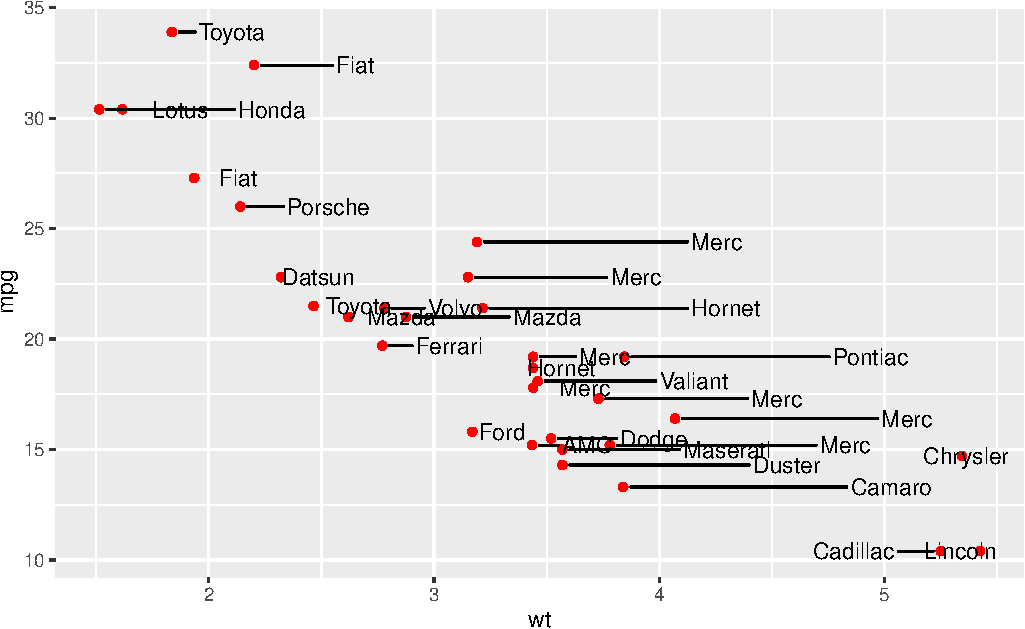
\includegraphics[width=\textwidth]{TRES-Tidy-Tutorial_files/figure-latex/unnamed-chunk-29-1} \end{center}

This is not a good looking plot, because it breaks other rules of plot design, such as whether this sort of plot should be made at all. Labels and text need to be applied sparingly, for example drawing attention or adding information to outliers.

\hypertarget{reshaping-data-tables-in-the-tidyverse-and-other-things}{%
\chapter{Reshaping data tables in the tidyverse, and other things}\label{reshaping-data-tables-in-the-tidyverse-and-other-things}}

Raphael Scherrer


\includegraphics{opening-image.png}

\begin{Shaded}
\begin{Highlighting}[]
\KeywordTok{library}\NormalTok{(tibble)}
\KeywordTok{library}\NormalTok{(tidyr)}
\end{Highlighting}
\end{Shaded}

In this chapter we will learn what \emph{tidy} means in the context of the tidyverse, and how to reshape our data into a tidy format using the \texttt{tidyr} package. But first, let us take a detour and introduce the \texttt{tibble}.

\hypertarget{the-new-data-frame-tibble}{%
\section{The new data frame: tibble}\label{the-new-data-frame-tibble}}

The \texttt{tibble} is the recommended class to use to store tabular data in the tidyverse. Consider it as the operational unit of any data science pipeline. For most practical purposes, a \texttt{tibble} is basically a \texttt{data.frame}.

\begin{Shaded}
\begin{Highlighting}[]
\CommentTok{# Make a data frame}
\KeywordTok{data.frame}\NormalTok{(}\DataTypeTok{who =} \KeywordTok{c}\NormalTok{(}\StringTok{"Pratik"}\NormalTok{, }\StringTok{"Theo"}\NormalTok{, }\StringTok{"Raph"}\NormalTok{), }\DataTypeTok{chapt =} \KeywordTok{c}\NormalTok{(}\StringTok{"1, 4"}\NormalTok{, }\StringTok{"3"}\NormalTok{, }\StringTok{"2, 5"}\NormalTok{))}
\CommentTok{#>      who chapt}
\CommentTok{#> 1 Pratik  1, 4}
\CommentTok{#> 2   Theo     3}
\CommentTok{#> 3   Raph  2, 5}

\CommentTok{# Or an equivalent tibble}
\KeywordTok{tibble}\NormalTok{(}\DataTypeTok{who =} \KeywordTok{c}\NormalTok{(}\StringTok{"Pratik"}\NormalTok{, }\StringTok{"Theo"}\NormalTok{, }\StringTok{"Raph"}\NormalTok{), }\DataTypeTok{chapt =} \KeywordTok{c}\NormalTok{(}\StringTok{"1, 4"}\NormalTok{, }\StringTok{"3"}\NormalTok{, }\StringTok{"2, 5"}\NormalTok{))}
\CommentTok{#> # A tibble: 3 x 2}
\CommentTok{#>   who    chapt}
\CommentTok{#>   <chr>  <chr>}
\CommentTok{#> 1 Pratik 1, 4 }
\CommentTok{#> 2 Theo   3    }
\CommentTok{#> 3 Raph   2, 5}
\end{Highlighting}
\end{Shaded}

The difference between \texttt{tibble} and \texttt{data.frame} is in its display and in the way it is subsetted, among others. Most functions working with \texttt{data.frame} will work with \texttt{tibble} and vice versa. Use the \texttt{as*} family of functions to switch back and forth between the two if needed, using e.g.~\texttt{as.data.frame} or \texttt{as\_tibble}.

In terms of display, the tibble has the advantage of showing the class of each column: \texttt{chr} for \texttt{character}, \texttt{fct} for \texttt{factor}, \texttt{int} for \texttt{integer}, \texttt{dbl} for \texttt{numeric} and \texttt{lgl} for \texttt{logical}, just to name the main atomic classes. This may be more important than you think, because many hard-to-find bugs in R are due to wrong variable types and/or cryptic type conversions. This especially happens with \texttt{factor} and \texttt{character}, which can cause quite some confusion. More about this in the extra section at the end of this chapter!

Note that you can build a tibble by rows rather than by columns with \texttt{tribble}:

\begin{Shaded}
\begin{Highlighting}[]
\KeywordTok{tribble}\NormalTok{(}
  \OperatorTok{~}\NormalTok{who, }\OperatorTok{~}\NormalTok{chapt,}
  \StringTok{"Pratik"}\NormalTok{, }\StringTok{"1, 4"}\NormalTok{,}
  \StringTok{"Theo"}\NormalTok{, }\StringTok{"3"}\NormalTok{,}
  \StringTok{"Raph"}\NormalTok{, }\StringTok{"2, 5"}
\NormalTok{)}
\CommentTok{#> # A tibble: 3 x 2}
\CommentTok{#>   who    chapt}
\CommentTok{#>   <chr>  <chr>}
\CommentTok{#> 1 Pratik 1, 4 }
\CommentTok{#> 2 Theo   3    }
\CommentTok{#> 3 Raph   2, 5}
\end{Highlighting}
\end{Shaded}

As a rule of thumb, try to convert your tables to tibbles whenever you can, especially when the original table is \emph{not} a data frame. For example, the principal component analysis function \texttt{prcomp} outputs a \texttt{matrix} of coordinates in principal component-space.

\begin{Shaded}
\begin{Highlighting}[]
\CommentTok{# Perform a PCA on mtcars }
\NormalTok{pca_scores <-}\StringTok{ }\KeywordTok{prcomp}\NormalTok{(mtcars)}\OperatorTok{$}\NormalTok{x}
\KeywordTok{head}\NormalTok{(pca_scores) }\CommentTok{# looks like a data frame or a tibble...}
\CommentTok{#>                       PC1   PC2   PC3    PC4    PC5     PC6      PC7     PC8}
\CommentTok{#> Mazda RX4          -79.60  2.13 -2.15 -2.707 -0.702 -0.3149 -0.09870 -0.0779}
\CommentTok{#> Mazda RX4 Wag      -79.60  2.15 -2.22 -2.178 -0.884 -0.4534 -0.00355 -0.0957}
\CommentTok{#> Datsun 710        -133.89 -5.06 -2.14  0.346  1.106  1.1730  0.00576  0.1362}
\CommentTok{#> Hornet 4 Drive       8.52 44.99  1.23  0.827  0.424 -0.0579 -0.02431  0.2212}
\CommentTok{#> Hornet Sportabout  128.69 30.82  3.34 -0.521  0.737 -0.3329  0.10630 -0.0530}
\CommentTok{#> Valiant            -23.22 35.11 -3.26  1.401  0.803 -0.0884  0.23895  0.4239}
\CommentTok{#>                      PC9    PC10   PC11}
\CommentTok{#> Mazda RX4         -0.200 -0.2901  0.106}
\CommentTok{#> Mazda RX4 Wag     -0.353 -0.1928  0.107}
\CommentTok{#> Datsun 710        -0.198  0.0763  0.267}
\CommentTok{#> Hornet 4 Drive     0.356 -0.0906  0.209}
\CommentTok{#> Hornet Sportabout  0.153 -0.1886 -0.109}
\CommentTok{#> Valiant            0.101 -0.0377  0.276}
\KeywordTok{class}\NormalTok{(pca_scores) }\CommentTok{# but is actually a matrix}
\CommentTok{#> [1] "matrix"}

\CommentTok{# Convert to tibble}
\KeywordTok{as_tibble}\NormalTok{(pca_scores)}
\CommentTok{#> # A tibble: 32 x 11}
\CommentTok{#>       PC1   PC2   PC3    PC4    PC5     PC6      PC7     PC8    PC9    PC10}
\CommentTok{#>     <dbl> <dbl> <dbl>  <dbl>  <dbl>   <dbl>    <dbl>   <dbl>  <dbl>   <dbl>}
\CommentTok{#> 1  -79.6   2.13 -2.15 -2.71  -0.702 -0.315  -0.0987  -0.0779 -0.200 -0.290 }
\CommentTok{#> 2  -79.6   2.15 -2.22 -2.18  -0.884 -0.453  -0.00355 -0.0957 -0.353 -0.193 }
\CommentTok{#> 3 -134.   -5.06 -2.14  0.346  1.11   1.17    0.00576  0.136  -0.198  0.0763}
\CommentTok{#> 4    8.52 45.0   1.23  0.827  0.424 -0.0579 -0.0243   0.221   0.356 -0.0906}
\CommentTok{#> 5  129.   30.8   3.34 -0.521  0.737 -0.333   0.106   -0.0530  0.153 -0.189 }
\CommentTok{#> 6  -23.2  35.1  -3.26  1.40   0.803 -0.0884  0.239    0.424   0.101 -0.0377}
\CommentTok{#> # ... with 26 more rows, and 1 more variable: PC11 <dbl>}
\end{Highlighting}
\end{Shaded}

This is important because a \texttt{matrix} can contain only one type of values (e.g.~only \texttt{numeric} or \texttt{character}), while \texttt{tibble} (and \texttt{data.frame}) allow you to have columns of different types.

So, in the tidyverse we are going to work with tibbles, got it. But what does ``tidy'' mean exactly?

\hypertarget{the-concept-of-tidy-data}{%
\section{The concept of tidy data}\label{the-concept-of-tidy-data}}

When it comes to putting data into tables, there are many ways one could organize a dataset. The \emph{tidy} format is one such format. According to the formal \href{https://tidyr.tidyverse.org/articles/tidy-data.html}{definition}, a table is tidy if each column is a variable and each row is an observation. In practice, however, I found that this is not a very operational definition, especially in ecology and evolution where we often record multiple variables per individual. So, let's dig in with an example.

Say we have a dataset of several morphometrics measured on Darwin's finches in the Galapagos islands. Let's first get this dataset.

\begin{Shaded}
\begin{Highlighting}[]
\CommentTok{# We first simulate random data}
\NormalTok{beak_lengths <-}\StringTok{ }\KeywordTok{rnorm}\NormalTok{(}\DecValTok{100}\NormalTok{, }\DataTypeTok{mean =} \DecValTok{5}\NormalTok{, }\DataTypeTok{sd =} \FloatTok{0.1}\NormalTok{)}
\NormalTok{beak_widths <-}\StringTok{ }\KeywordTok{rnorm}\NormalTok{(}\DecValTok{100}\NormalTok{, }\DataTypeTok{mean =} \DecValTok{2}\NormalTok{, }\DataTypeTok{sd =} \FloatTok{0.1}\NormalTok{)}
\NormalTok{body_weights <-}\StringTok{ }\KeywordTok{rgamma}\NormalTok{(}\DecValTok{100}\NormalTok{, }\DataTypeTok{shape =} \DecValTok{10}\NormalTok{, }\DataTypeTok{rate =} \DecValTok{1}\NormalTok{)}
\NormalTok{islands <-}\StringTok{ }\KeywordTok{rep}\NormalTok{(}\KeywordTok{c}\NormalTok{(}\StringTok{"Isabela"}\NormalTok{, }\StringTok{"Santa Cruz"}\NormalTok{), }\DataTypeTok{each =} \DecValTok{50}\NormalTok{)}

\CommentTok{# Assemble into a tibble}
\NormalTok{data <-}\StringTok{ }\KeywordTok{tibble}\NormalTok{(}
  \DataTypeTok{id =} \DecValTok{1}\OperatorTok{:}\DecValTok{100}\NormalTok{,}
  \DataTypeTok{body_weight =}\NormalTok{ body_weights,}
  \DataTypeTok{beak_length =}\NormalTok{ beak_lengths,  }
  \DataTypeTok{beak_width =}\NormalTok{ beak_widths,}
  \DataTypeTok{island =}\NormalTok{ islands}
\NormalTok{)}

\CommentTok{# Snapshot}
\NormalTok{data}
\CommentTok{#> # A tibble: 100 x 5}
\CommentTok{#>      id body_weight beak_length beak_width island }
\CommentTok{#>   <int>       <dbl>       <dbl>      <dbl> <chr>  }
\CommentTok{#> 1     1       10.8         4.94       1.94 Isabela}
\CommentTok{#> 2     2       15.4         5.02       2.00 Isabela}
\CommentTok{#> 3     3       15.0         4.92       1.91 Isabela}
\CommentTok{#> 4     4        8.51        5.16       2.02 Isabela}
\CommentTok{#> 5     5       14.9         5.03       1.93 Isabela}
\CommentTok{#> 6     6        8.41        4.92       2.18 Isabela}
\CommentTok{#> # ... with 94 more rows}
\end{Highlighting}
\end{Shaded}

Here, we pretend to have measured \texttt{beak\_length}, \texttt{beak\_width} and \texttt{body\_weight} on 100 birds, 50 of them from Isabela and 50 of them from Santa Cruz. In this tibble, each row is an individual bird. This is probably the way most scientists would record their data in the field. However, a single bird is not an ``observation'' in the sense used in the tidyverse. Our dataset is not tidy but \emph{messy}.

The tidy equivalent of this dataset would be:

\begin{Shaded}
\begin{Highlighting}[]
\NormalTok{data <-}\StringTok{ }\KeywordTok{pivot_longer}\NormalTok{(}
\NormalTok{  data, }
  \DataTypeTok{cols =} \KeywordTok{c}\NormalTok{(}\StringTok{"body_weight"}\NormalTok{, }\StringTok{"beak_length"}\NormalTok{, }\StringTok{"beak_width"}\NormalTok{),}
  \DataTypeTok{names_to =} \StringTok{"variable"}
\NormalTok{)}
\NormalTok{data}
\CommentTok{#> # A tibble: 300 x 4}
\CommentTok{#>      id island  variable    value}
\CommentTok{#>   <int> <chr>   <chr>       <dbl>}
\CommentTok{#> 1     1 Isabela body_weight 10.8 }
\CommentTok{#> 2     1 Isabela beak_length  4.94}
\CommentTok{#> 3     1 Isabela beak_width   1.94}
\CommentTok{#> 4     2 Isabela body_weight 15.4 }
\CommentTok{#> 5     2 Isabela beak_length  5.02}
\CommentTok{#> 6     2 Isabela beak_width   2.00}
\CommentTok{#> # ... with 294 more rows}
\end{Highlighting}
\end{Shaded}

where each \emph{measurement} (and not each \emph{individual}) is now the unit of observation (the rows). The \texttt{pivot\_longer} function is the easiest way to get to this format. It belongs to the \texttt{tidyr} package, which we'll cover in a minute.

As you can see our tibble now has three times as many rows and fewer columns. This format is rather unintuitive and not optimal for display. However, it provides a very standardized and consistent way of organizing data that will be understood (and expected) by pretty much all functions in the tidyverse. This makes the tidyverse tools work well together and reduces the time you would otherwise spend reformatting your data from one tool to the next.

That does not mean that the \emph{messy} format is useless though. There may be use-cases where you need to switch back and forth between formats. For this reason I prefer referring to these formats using their other names: \emph{long} (tidy) versus \emph{wide} (messy). For example, matrix operations work much faster on wide data, and the wide format arguably looks nicer for display. Luckily the \texttt{tidyr} package gives us the tools to reshape our data as needed, as we shall see shortly.

Another common example of wide-or-long dilemma is when dealing with \emph{contingency tables}. This would be our case, for example, if we asked how many observations we have for each morphometric and each island. We use \texttt{table} (from base R) to get the answer:

\begin{Shaded}
\begin{Highlighting}[]
\CommentTok{# Make a contingency table}
\NormalTok{ctg <-}\StringTok{ }\KeywordTok{with}\NormalTok{(data, }\KeywordTok{table}\NormalTok{(island, variable))}
\NormalTok{ctg}
\CommentTok{#>             variable}
\CommentTok{#> island       beak_length beak_width body_weight}
\CommentTok{#>   Isabela             50         50          50}
\CommentTok{#>   Santa Cruz          50         50          50}
\end{Highlighting}
\end{Shaded}

A variety of statistical tests can be used on contingency tables such as Fisher's exact test, the chi-square test or the binomial test. Contingency tables are in the wide format by construction, but they too can be pivoted to the long format, and the tidyverse manipulation tools will expect you to do so. Actually, \texttt{tibble} knows that very well and does it by default if you convert your \texttt{table} into a \texttt{tibble}:

\begin{Shaded}
\begin{Highlighting}[]
\CommentTok{# Contingency table is pivoted to the long-format automatically}
\KeywordTok{as_tibble}\NormalTok{(ctg)}
\CommentTok{#> # A tibble: 6 x 3}
\CommentTok{#>   island     variable        n}
\CommentTok{#>   <chr>      <chr>       <int>}
\CommentTok{#> 1 Isabela    beak_length    50}
\CommentTok{#> 2 Santa Cruz beak_length    50}
\CommentTok{#> 3 Isabela    beak_width     50}
\CommentTok{#> 4 Santa Cruz beak_width     50}
\CommentTok{#> 5 Isabela    body_weight    50}
\CommentTok{#> 6 Santa Cruz body_weight    50}
\end{Highlighting}
\end{Shaded}

\begin{infobox}{summary}

\emph{Summary: Tidy or not tidy}

To sum up, the definition of what is tidy and what is not is somewhat subjective. Tables can be in long or wide format, and depending on the complexity of a dataset, there may even be some intermediate states. To be clear, the tidyverse does not only accept long tables, and wide tables may sometimes be the way to go. This is very use-case specific. Have a clear idea of what you want to do with your data (what tidyverse tools you will use), and use that to figure which format makes more sense. And remember, \texttt{tidyr} is here to easily do the switching for you.

\end{infobox}

\hypertarget{reshaping-with-tidyr}{%
\section{\texorpdfstring{Reshaping with \texttt{tidyr}}{Reshaping with tidyr}}\label{reshaping-with-tidyr}}

The \texttt{tidyr} package implements tools to easily switch between layouts and also perform a few other reshaping operations. Old school R users will be familiar with the \texttt{reshape} and \texttt{reshape2} packages, of which \texttt{tidyr} is the tidyverse equivalent. Beware that \texttt{tidyr} is about playing with the general \emph{layout} of the dataset, while \emph{operations} and \emph{transformations} of the data are within the scope of the \texttt{dplyr} and \texttt{purrr} packages. All these packages work hand-in-hand really well, and analysis pipelines usually involve all of them. But today, we focus on the first member of this holy trinity, which is often the first one you'll need because you will want to reshape your data before doing other things. So, please hold your non-layout-related questions for the next chapters.

\hypertarget{pivoting}{%
\subsection{Pivoting}\label{pivoting}}

Pivoting a dataset between the long and wide layout is the main purpose of \texttt{tidyr} (check out the package's logo). We already saw the \texttt{pivot\_longer} function above. This function converts a table form wide to long format. Similarly, there is a \texttt{pivot\_wider} function that does exactly the opposite and takes you back to the wide format:

\begin{Shaded}
\begin{Highlighting}[]
\KeywordTok{pivot_wider}\NormalTok{(}
\NormalTok{  data, }
  \DataTypeTok{names_from =} \StringTok{"variable"}\NormalTok{, }
  \DataTypeTok{values_from =} \StringTok{"value"}\NormalTok{, }
  \DataTypeTok{id_cols =} \KeywordTok{c}\NormalTok{(}\StringTok{"id"}\NormalTok{, }\StringTok{"island"}\NormalTok{)}
\NormalTok{)}
\CommentTok{#> # A tibble: 100 x 5}
\CommentTok{#>      id island  body_weight beak_length beak_width}
\CommentTok{#>   <int> <chr>         <dbl>       <dbl>      <dbl>}
\CommentTok{#> 1     1 Isabela       10.8         4.94       1.94}
\CommentTok{#> 2     2 Isabela       15.4         5.02       2.00}
\CommentTok{#> 3     3 Isabela       15.0         4.92       1.91}
\CommentTok{#> 4     4 Isabela        8.51        5.16       2.02}
\CommentTok{#> 5     5 Isabela       14.9         5.03       1.93}
\CommentTok{#> 6     6 Isabela        8.41        4.92       2.18}
\CommentTok{#> # ... with 94 more rows}
\end{Highlighting}
\end{Shaded}

The order of the columns is not exactly as it was, but this should not matter in a data analysis pipeline where you should access columns by their names. It is straightforward to change the order of the columns, but this is more within the scope of the \texttt{dplyr} package.

If you are familiar with earlier versions of the tidyverse, \texttt{pivot\_longer} and \texttt{pivot\_wider} are the respective equivalents of \texttt{gather} and \texttt{spread}, which are now deprecated.

There are a few other reshaping operations from \texttt{tidyr} that are worth knowing.

\hypertarget{handling-missing-values}{%
\subsection{Handling missing values}\label{handling-missing-values}}

Say we have some missing measurements in the column ``value'' of our finch dataset:

\begin{Shaded}
\begin{Highlighting}[]
\CommentTok{# We replace 100 random observations by NAs}
\NormalTok{ii <-}\StringTok{ }\KeywordTok{sample}\NormalTok{(}\KeywordTok{nrow}\NormalTok{(data), }\DecValTok{100}\NormalTok{)}
\NormalTok{data}\OperatorTok{$}\NormalTok{value[ii] <-}\StringTok{ }\OtherTok{NA}
\NormalTok{data}
\CommentTok{#> # A tibble: 300 x 4}
\CommentTok{#>      id island  variable    value}
\CommentTok{#>   <int> <chr>   <chr>       <dbl>}
\CommentTok{#> 1     1 Isabela body_weight 10.8 }
\CommentTok{#> 2     1 Isabela beak_length NA   }
\CommentTok{#> 3     1 Isabela beak_width  NA   }
\CommentTok{#> 4     2 Isabela body_weight NA   }
\CommentTok{#> 5     2 Isabela beak_length  5.02}
\CommentTok{#> 6     2 Isabela beak_width  NA   }
\CommentTok{#> # ... with 294 more rows}
\end{Highlighting}
\end{Shaded}

We could get rid of the rows that have missing values using \texttt{drop\_na}:

\begin{Shaded}
\begin{Highlighting}[]
\KeywordTok{drop_na}\NormalTok{(data, value)}
\CommentTok{#> # A tibble: 200 x 4}
\CommentTok{#>      id island  variable    value}
\CommentTok{#>   <int> <chr>   <chr>       <dbl>}
\CommentTok{#> 1     1 Isabela body_weight 10.8 }
\CommentTok{#> 2     2 Isabela beak_length  5.02}
\CommentTok{#> 3     3 Isabela body_weight 15.0 }
\CommentTok{#> 4     3 Isabela beak_length  4.92}
\CommentTok{#> 5     4 Isabela body_weight  8.51}
\CommentTok{#> 6     4 Isabela beak_width   2.02}
\CommentTok{#> # ... with 194 more rows}
\end{Highlighting}
\end{Shaded}

Else, we could replace the NAs with some user-defined value:

\begin{Shaded}
\begin{Highlighting}[]
\KeywordTok{replace_na}\NormalTok{(data, }\DataTypeTok{replace =} \KeywordTok{list}\NormalTok{(}\DataTypeTok{value =} \DecValTok{-999}\NormalTok{))}
\CommentTok{#> # A tibble: 300 x 4}
\CommentTok{#>      id island  variable      value}
\CommentTok{#>   <int> <chr>   <chr>         <dbl>}
\CommentTok{#> 1     1 Isabela body_weight   10.8 }
\CommentTok{#> 2     1 Isabela beak_length -999   }
\CommentTok{#> 3     1 Isabela beak_width  -999   }
\CommentTok{#> 4     2 Isabela body_weight -999   }
\CommentTok{#> 5     2 Isabela beak_length    5.02}
\CommentTok{#> 6     2 Isabela beak_width  -999   }
\CommentTok{#> # ... with 294 more rows}
\end{Highlighting}
\end{Shaded}

where the \texttt{replace} argument takes a named list, and the names should refer to the columns to apply the replacement to.

We could also replace NAs with the most recent non-NA values:

\begin{Shaded}
\begin{Highlighting}[]
\KeywordTok{fill}\NormalTok{(data, value)}
\CommentTok{#> # A tibble: 300 x 4}
\CommentTok{#>      id island  variable    value}
\CommentTok{#>   <int> <chr>   <chr>       <dbl>}
\CommentTok{#> 1     1 Isabela body_weight 10.8 }
\CommentTok{#> 2     1 Isabela beak_length 10.8 }
\CommentTok{#> 3     1 Isabela beak_width  10.8 }
\CommentTok{#> 4     2 Isabela body_weight 10.8 }
\CommentTok{#> 5     2 Isabela beak_length  5.02}
\CommentTok{#> 6     2 Isabela beak_width   5.02}
\CommentTok{#> # ... with 294 more rows}
\end{Highlighting}
\end{Shaded}

Note that most functions in the tidyverse take a tibble as their first argument, and columns to which to apply the functions are usually passed as ``objects'' rather than character strings. In the above example, we passed the \texttt{value} column as \texttt{value}, not \texttt{"value"}. These column-objects are called by the tidyverse functions \emph{in the context} of the data (the tibble) they belong to.

\hypertarget{splitting-and-combining-cells}{%
\subsection{Splitting and combining cells}\label{splitting-and-combining-cells}}

The \texttt{tidyr} package offers tools to split and combine columns. This is a nice extension to the string manipulations we saw last week in the \texttt{stringr} tutorial.

Say we want to add the specific dates when we took measurements on our birds (we would normally do this using \texttt{dplyr} but for now we will stick to the old way):

\begin{Shaded}
\begin{Highlighting}[]
\CommentTok{# Sample random dates for each observation}
\NormalTok{data}\OperatorTok{$}\NormalTok{day <-}\StringTok{ }\KeywordTok{sample}\NormalTok{(}\DecValTok{30}\NormalTok{, }\KeywordTok{nrow}\NormalTok{(data), }\DataTypeTok{replace =} \OtherTok{TRUE}\NormalTok{)}
\NormalTok{data}\OperatorTok{$}\NormalTok{month <-}\StringTok{ }\KeywordTok{sample}\NormalTok{(}\DecValTok{12}\NormalTok{, }\KeywordTok{nrow}\NormalTok{(data), }\DataTypeTok{replace =} \OtherTok{TRUE}\NormalTok{)}
\NormalTok{data}\OperatorTok{$}\NormalTok{year <-}\StringTok{ }\KeywordTok{sample}\NormalTok{(}\DecValTok{2019}\OperatorTok{:}\DecValTok{2020}\NormalTok{, }\KeywordTok{nrow}\NormalTok{(data), }\DataTypeTok{replace =} \OtherTok{TRUE}\NormalTok{)}
\NormalTok{data}
\CommentTok{#> # A tibble: 300 x 7}
\CommentTok{#>      id island  variable    value   day month  year}
\CommentTok{#>   <int> <chr>   <chr>       <dbl> <int> <int> <int>}
\CommentTok{#> 1     1 Isabela body_weight 10.8      8     7  2020}
\CommentTok{#> 2     1 Isabela beak_length NA       19     7  2019}
\CommentTok{#> 3     1 Isabela beak_width  NA       17    12  2019}
\CommentTok{#> 4     2 Isabela body_weight NA       20    12  2020}
\CommentTok{#> 5     2 Isabela beak_length  5.02    21    10  2020}
\CommentTok{#> 6     2 Isabela beak_width  NA       23     2  2020}
\CommentTok{#> # ... with 294 more rows}
\end{Highlighting}
\end{Shaded}

We could combine the \texttt{day}, \texttt{month} and \texttt{year} columns into a single \texttt{date} column, with a dash as a separator, using \texttt{unite}:

\begin{Shaded}
\begin{Highlighting}[]
\NormalTok{data <-}\StringTok{ }\KeywordTok{unite}\NormalTok{(data, day, month, year, }\DataTypeTok{col =} \StringTok{"date"}\NormalTok{, }\DataTypeTok{sep =} \StringTok{"-"}\NormalTok{)}
\NormalTok{data}
\CommentTok{#> # A tibble: 300 x 5}
\CommentTok{#>      id island  variable    value date      }
\CommentTok{#>   <int> <chr>   <chr>       <dbl> <chr>     }
\CommentTok{#> 1     1 Isabela body_weight 10.8  8-7-2020  }
\CommentTok{#> 2     1 Isabela beak_length NA    19-7-2019 }
\CommentTok{#> 3     1 Isabela beak_width  NA    17-12-2019}
\CommentTok{#> 4     2 Isabela body_weight NA    20-12-2020}
\CommentTok{#> 5     2 Isabela beak_length  5.02 21-10-2020}
\CommentTok{#> 6     2 Isabela beak_width  NA    23-2-2020 }
\CommentTok{#> # ... with 294 more rows}
\end{Highlighting}
\end{Shaded}

Of course, we can revert back to the previous dataset by splitting the \texttt{date} column with \texttt{separate}.

\begin{Shaded}
\begin{Highlighting}[]
\KeywordTok{separate}\NormalTok{(data, date, }\DataTypeTok{into =} \KeywordTok{c}\NormalTok{(}\StringTok{"day"}\NormalTok{, }\StringTok{"month"}\NormalTok{, }\StringTok{"year"}\NormalTok{))}
\CommentTok{#> # A tibble: 300 x 7}
\CommentTok{#>      id island  variable    value day   month year }
\CommentTok{#>   <int> <chr>   <chr>       <dbl> <chr> <chr> <chr>}
\CommentTok{#> 1     1 Isabela body_weight 10.8  8     7     2020 }
\CommentTok{#> 2     1 Isabela beak_length NA    19    7     2019 }
\CommentTok{#> 3     1 Isabela beak_width  NA    17    12    2019 }
\CommentTok{#> 4     2 Isabela body_weight NA    20    12    2020 }
\CommentTok{#> 5     2 Isabela beak_length  5.02 21    10    2020 }
\CommentTok{#> 6     2 Isabela beak_width  NA    23    2     2020 }
\CommentTok{#> # ... with 294 more rows}
\end{Highlighting}
\end{Shaded}

But note that the \texttt{day}, \texttt{month} and \texttt{year} columns are now of class \texttt{character} and not \texttt{integer} anymore. This is because they result from the splitting of \texttt{date}, which itself was a \texttt{character} column.

You can also separate a single column into multiple \emph{rows} using \texttt{separate\_rows}:

\begin{Shaded}
\begin{Highlighting}[]
\KeywordTok{separate_rows}\NormalTok{(data, date)}
\CommentTok{#> # A tibble: 900 x 5}
\CommentTok{#>      id island  variable    value date }
\CommentTok{#>   <int> <chr>   <chr>       <dbl> <chr>}
\CommentTok{#> 1     1 Isabela body_weight  10.8 8    }
\CommentTok{#> 2     1 Isabela body_weight  10.8 7    }
\CommentTok{#> 3     1 Isabela body_weight  10.8 2020 }
\CommentTok{#> 4     1 Isabela beak_length  NA   19   }
\CommentTok{#> 5     1 Isabela beak_length  NA   7    }
\CommentTok{#> 6     1 Isabela beak_length  NA   2019 }
\CommentTok{#> # ... with 894 more rows}
\end{Highlighting}
\end{Shaded}

\hypertarget{expanding-tables-using-combinations}{%
\subsection{Expanding tables using combinations}\label{expanding-tables-using-combinations}}

Instead of getting rid of rows with NAs, we may want to add rows with NAs, for example, for combinations of parameters that we did not measure.

\begin{Shaded}
\begin{Highlighting}[]
\NormalTok{data <-}\StringTok{ }\KeywordTok{separate}\NormalTok{(data, date, }\DataTypeTok{into =} \KeywordTok{c}\NormalTok{(}\StringTok{"day"}\NormalTok{, }\StringTok{"month"}\NormalTok{, }\StringTok{"year"}\NormalTok{))}
\NormalTok{to_rm <-}\StringTok{ }\KeywordTok{with}\NormalTok{(data, island }\OperatorTok{==}\StringTok{ "Santa Cruz"} \OperatorTok{&}\StringTok{ }\NormalTok{year }\OperatorTok{==}\StringTok{ "2020"}\NormalTok{)}
\NormalTok{data <-}\StringTok{ }\NormalTok{data[}\OperatorTok{!}\NormalTok{to_rm,]}
\KeywordTok{tail}\NormalTok{(data)}
\CommentTok{#> # A tibble: 6 x 7}
\CommentTok{#>      id island     variable    value day   month year }
\CommentTok{#>   <int> <chr>      <chr>       <dbl> <chr> <chr> <chr>}
\CommentTok{#> 1    98 Santa Cruz beak_length  4.94 22    12    2019 }
\CommentTok{#> 2    98 Santa Cruz beak_width   1.90 9     1     2019 }
\CommentTok{#> 3    99 Santa Cruz body_weight 15.0  16    7     2019 }
\CommentTok{#> 4    99 Santa Cruz beak_length NA    26    10    2019 }
\CommentTok{#> 5    99 Santa Cruz beak_width   2.04 30    7     2019 }
\CommentTok{#> 6   100 Santa Cruz beak_width  NA    23    3     2019}
\end{Highlighting}
\end{Shaded}

We could generate a tibble with all combinations of island, morphometric and year using \texttt{expand\_grid}:

\begin{Shaded}
\begin{Highlighting}[]
\KeywordTok{expand_grid}\NormalTok{(}
  \DataTypeTok{island =} \KeywordTok{c}\NormalTok{(}\StringTok{"Isabela"}\NormalTok{, }\StringTok{"Santa Cruz"}\NormalTok{), }
  \DataTypeTok{year =} \KeywordTok{c}\NormalTok{(}\StringTok{"2019"}\NormalTok{, }\StringTok{"2020"}\NormalTok{)}
\NormalTok{)}
\CommentTok{#> # A tibble: 4 x 2}
\CommentTok{#>   island     year }
\CommentTok{#>   <chr>      <chr>}
\CommentTok{#> 1 Isabela    2019 }
\CommentTok{#> 2 Isabela    2020 }
\CommentTok{#> 3 Santa Cruz 2019 }
\CommentTok{#> 4 Santa Cruz 2020}
\end{Highlighting}
\end{Shaded}

If we already have a tibble to work from that contains the variables to combine, we can use \texttt{expand} on that tibble:

\begin{Shaded}
\begin{Highlighting}[]
\KeywordTok{expand}\NormalTok{(data, island, year)}
\CommentTok{#> # A tibble: 4 x 2}
\CommentTok{#>   island     year }
\CommentTok{#>   <chr>      <chr>}
\CommentTok{#> 1 Isabela    2019 }
\CommentTok{#> 2 Isabela    2020 }
\CommentTok{#> 3 Santa Cruz 2019 }
\CommentTok{#> 4 Santa Cruz 2020}
\end{Highlighting}
\end{Shaded}

As you can see, we get all the combinations of the variables of interest, even those that are missing. But sometimes you might be interested in variables that are \emph{nested} within each other and not \emph{crossed}. For example, say we have measured birds at different locations within each island:

\begin{Shaded}
\begin{Highlighting}[]
\NormalTok{nrow_Isabela <-}\StringTok{ }\KeywordTok{with}\NormalTok{(data, }\KeywordTok{length}\NormalTok{(}\KeywordTok{which}\NormalTok{(island }\OperatorTok{==}\StringTok{ "Isabela"}\NormalTok{)))}
\NormalTok{nrow_SantaCruz <-}\StringTok{ }\KeywordTok{with}\NormalTok{(data, }\KeywordTok{length}\NormalTok{(}\KeywordTok{which}\NormalTok{(island }\OperatorTok{==}\StringTok{ "Santa Cruz"}\NormalTok{)))}
\NormalTok{sites_Isabela <-}\StringTok{ }\KeywordTok{sample}\NormalTok{(}\KeywordTok{c}\NormalTok{(}\StringTok{"A"}\NormalTok{, }\StringTok{"B"}\NormalTok{), }\DataTypeTok{size =}\NormalTok{ nrow_Isabela, }\DataTypeTok{replace =} \OtherTok{TRUE}\NormalTok{)}
\NormalTok{sites_SantaCruz <-}\StringTok{ }\KeywordTok{sample}\NormalTok{(}\KeywordTok{c}\NormalTok{(}\StringTok{"C"}\NormalTok{, }\StringTok{"D"}\NormalTok{), }\DataTypeTok{size =}\NormalTok{ nrow_SantaCruz, }\DataTypeTok{replace =} \OtherTok{TRUE}\NormalTok{)}
\NormalTok{sites <-}\StringTok{ }\KeywordTok{c}\NormalTok{(sites_Isabela, sites_SantaCruz)}
\NormalTok{data}\OperatorTok{$}\NormalTok{site <-}\StringTok{ }\NormalTok{sites}
\NormalTok{data}
\CommentTok{#> # A tibble: 232 x 8}
\CommentTok{#>      id island  variable    value day   month year  site }
\CommentTok{#>   <int> <chr>   <chr>       <dbl> <chr> <chr> <chr> <chr>}
\CommentTok{#> 1     1 Isabela body_weight 10.8  8     7     2020  A    }
\CommentTok{#> 2     1 Isabela beak_length NA    19    7     2019  B    }
\CommentTok{#> 3     1 Isabela beak_width  NA    17    12    2019  B    }
\CommentTok{#> 4     2 Isabela body_weight NA    20    12    2020  A    }
\CommentTok{#> 5     2 Isabela beak_length  5.02 21    10    2020  A    }
\CommentTok{#> 6     2 Isabela beak_width  NA    23    2     2020  A    }
\CommentTok{#> # ... with 226 more rows}
\end{Highlighting}
\end{Shaded}

Of course, if sites A and B are on Isabela, they cannot be on Santa Cruz, where we have sites C and D instead. It would not make sense to \texttt{expand} assuming that \texttt{island} and \texttt{site} are crossed, instead, they are nested. We can therefore expand using the \texttt{nesting} function:

\begin{Shaded}
\begin{Highlighting}[]
\KeywordTok{expand}\NormalTok{(data, }\KeywordTok{nesting}\NormalTok{(island, site, year))}
\CommentTok{#> # A tibble: 6 x 3}
\CommentTok{#>   island     site  year }
\CommentTok{#>   <chr>      <chr> <chr>}
\CommentTok{#> 1 Isabela    A     2019 }
\CommentTok{#> 2 Isabela    A     2020 }
\CommentTok{#> 3 Isabela    B     2019 }
\CommentTok{#> 4 Isabela    B     2020 }
\CommentTok{#> 5 Santa Cruz C     2019 }
\CommentTok{#> 6 Santa Cruz D     2019}
\end{Highlighting}
\end{Shaded}

But now the missing data for Santa Cruz in 2020 are not accounted for because \texttt{expand} thinks the \texttt{year} is also nested within island. To get back the missing combination, we use \texttt{crossing}, the complement of \texttt{nesting}:

\begin{Shaded}
\begin{Highlighting}[]
\KeywordTok{expand}\NormalTok{(data, }\KeywordTok{crossing}\NormalTok{(}\KeywordTok{nesting}\NormalTok{(island, site), year)) }\CommentTok{# both can be used together}
\CommentTok{#> # A tibble: 8 x 3}
\CommentTok{#>   island     site  year }
\CommentTok{#>   <chr>      <chr> <chr>}
\CommentTok{#> 1 Isabela    A     2019 }
\CommentTok{#> 2 Isabela    A     2020 }
\CommentTok{#> 3 Isabela    B     2019 }
\CommentTok{#> 4 Isabela    B     2020 }
\CommentTok{#> 5 Santa Cruz C     2019 }
\CommentTok{#> 6 Santa Cruz C     2020 }
\CommentTok{#> # ... with 2 more rows}
\end{Highlighting}
\end{Shaded}

Here, we specify that \texttt{site} is nested within \texttt{island} and these two are crossed with \texttt{year}. Easy!

But wait a minute. These combinations are all very good, but our measurements have disappeared! We can get them back by levelling up to the \texttt{complete} function instead of using \texttt{expand}:

\begin{Shaded}
\begin{Highlighting}[]
\KeywordTok{tail}\NormalTok{(}\KeywordTok{complete}\NormalTok{(data, }\KeywordTok{crossing}\NormalTok{(}\KeywordTok{nesting}\NormalTok{(island, site), year))) }
\CommentTok{#> # A tibble: 6 x 8}
\CommentTok{#>   island     site  year     id variable    value day   month}
\CommentTok{#>   <chr>      <chr> <chr> <int> <chr>       <dbl> <chr> <chr>}
\CommentTok{#> 1 Santa Cruz D     2019     95 beak_width  NA    13    10   }
\CommentTok{#> 2 Santa Cruz D     2019     98 beak_length  4.94 22    12   }
\CommentTok{#> 3 Santa Cruz D     2019     99 body_weight 15.0  16    7    }
\CommentTok{#> 4 Santa Cruz D     2019     99 beak_length NA    26    10   }
\CommentTok{#> 5 Santa Cruz D     2019     99 beak_width   2.04 30    7    }
\CommentTok{#> 6 Santa Cruz D     2020     NA <NA>        NA    <NA>  <NA>}
\CommentTok{# the last row has been added, full of NAs}
\end{Highlighting}
\end{Shaded}

which nicely keeps the rest of the columns in the tibble and just adds the missing combinations.

\hypertarget{nesting}{%
\subsection{Nesting}\label{nesting}}

The \texttt{tidyr} package has yet another feature that makes the tidyverse very powerful: the \texttt{nest} function. However, it makes little sense without combining it with the functions in the \texttt{purrr} package, so we will not cover it in this chapter but rather in the \texttt{purrr} chapter.

\hypertarget{what-else-can-be-tidied-up}{%
\subsection{What else can be tidied up?}\label{what-else-can-be-tidied-up}}

\hypertarget{model-output-with-broom}{%
\subsubsection{\texorpdfstring{Model output with \texttt{broom}}{Model output with broom}}\label{model-output-with-broom}}

Check out the \href{https://cran.r-project.org/web/packages/broom/vignettes/broom.html}{\texttt{broom}} package and its \texttt{tidy} function to tidy up messy linear model output, e.g.

\begin{Shaded}
\begin{Highlighting}[]
\KeywordTok{library}\NormalTok{(broom)}
\NormalTok{fit <-}\StringTok{ }\KeywordTok{lm}\NormalTok{(mpg }\OperatorTok{~}\StringTok{ }\NormalTok{cyl, mtcars)}
\KeywordTok{summary}\NormalTok{(fit)}
\CommentTok{#> }
\CommentTok{#> Call:}
\CommentTok{#> lm(formula = mpg ~ cyl, data = mtcars)}
\CommentTok{#> }
\CommentTok{#> Residuals:}
\CommentTok{#>    Min     1Q Median     3Q    Max }
\CommentTok{#> -4.981 -2.119  0.222  1.072  7.519 }
\CommentTok{#> }
\CommentTok{#> Coefficients:}
\CommentTok{#>             Estimate Std. Error t value Pr(>|t|)    }
\CommentTok{#> (Intercept)   37.885      2.074   18.27  < 2e-16 ***}
\CommentTok{#> cyl           -2.876      0.322   -8.92  6.1e-10 ***}
\CommentTok{#> ---}
\CommentTok{#> Signif. codes:  0 '***' 0.001 '**' 0.01 '*' 0.05 '.' 0.1 ' ' 1}
\CommentTok{#> }
\CommentTok{#> Residual standard error: 3.21 on 30 degrees of freedom}
\CommentTok{#> Multiple R-squared:  0.726,  Adjusted R-squared:  0.717 }
\CommentTok{#> F-statistic: 79.6 on 1 and 30 DF,  p-value: 6.11e-10}
\KeywordTok{tidy}\NormalTok{(fit) }\CommentTok{# returns a tibble}
\CommentTok{#> # A tibble: 2 x 5}
\CommentTok{#>   term        estimate std.error statistic  p.value}
\CommentTok{#>   <chr>          <dbl>     <dbl>     <dbl>    <dbl>}
\CommentTok{#> 1 (Intercept)    37.9      2.07      18.3  8.37e-18}
\CommentTok{#> 2 cyl            -2.88     0.322     -8.92 6.11e-10}
\end{Highlighting}
\end{Shaded}

The \texttt{broom} package is just one package among a series of packages together known as \href{https://www.tidymodels.org/}{tidymodels} that deal with statistical models according to the tidyverse philosophy, and those include machine learning models.

\hypertarget{graphs-with-tidygraph}{%
\subsubsection{\texorpdfstring{Graphs with \texttt{tidygraph}}{Graphs with tidygraph}}\label{graphs-with-tidygraph}}

For some datasets, sometimes there is no trivial and intuitive way to store them into a table. This is the case, for example, for data underlying graphs (as in networks), which contain information about relations between entities. What is the unit of observation in a network? A node? An edge between two nodes? Nodes and edges in a network may each have node- or edge-specific variables mapped to them, and both may be equally valid units of observation. The \href{https://www.data-imaginist.com/2017/introducing-tidygraph/}{\texttt{tidygraph}} package has tools to store graph-data in a tidyverse-friendly object, consisting of two tibbles: one for node-specific information, the other for edge-specific information. This package goes hand in hand with the \href{https://ggraph.data-imaginist.com/}{\texttt{ggraph}}, that makes plotting networks compatible with the grammar of graphics.

\hypertarget{trees-with-tidytree}{%
\subsubsection{\texorpdfstring{Trees with \texttt{tidytree}}{Trees with tidytree}}\label{trees-with-tidytree}}

Phylogenetic trees are a special type of graphs suffering from the same issue, i.e.~of being non-trivial to store in a table. The \href{https://yulab-smu.github.io/treedata-book/}{\texttt{tidytree}} package and its companion \texttt{treeio} offer an interface to convert tree-like objects (from most format used by other packages and software) into a tidyverse-friendly format. Again, the point is that the rest of the tidyverse can be used to wrangle or plot this type of data in the same way as one would do with regular tabular data. For plotting a \texttt{tidytree} with the grammar of graphics, see \href{https://guangchuangyu.github.io/ggtree-book/chapter-ggtree.html}{\texttt{ggtree}}.

\hypertarget{extra-factors-and-the-forcats-package}{%
\section{\texorpdfstring{Extra: factors and the \texttt{forcats} package}{Extra: factors and the forcats package}}\label{extra-factors-and-the-forcats-package}}

\begin{Shaded}
\begin{Highlighting}[]
\KeywordTok{library}\NormalTok{(forcats)}
\end{Highlighting}
\end{Shaded}

Categorical variables can be stored in R as character strings in \texttt{character} or \texttt{factor} objects. A \texttt{factor} looks like a \texttt{character}, but it actually is an \texttt{integer} vector, where each \texttt{integer} is mapped to a \texttt{character} label. With this respect it is sort of an enhanced version of \texttt{character}. For example,

\begin{Shaded}
\begin{Highlighting}[]
\NormalTok{my_char_vec <-}\StringTok{ }\KeywordTok{c}\NormalTok{(}\StringTok{"Pratik"}\NormalTok{, }\StringTok{"Theo"}\NormalTok{, }\StringTok{"Raph"}\NormalTok{)}
\NormalTok{my_char_vec}
\CommentTok{#> [1] "Pratik" "Theo"   "Raph"}
\end{Highlighting}
\end{Shaded}

is a \texttt{character} vector, recognizable to its double quotes, while

\begin{Shaded}
\begin{Highlighting}[]
\NormalTok{my_fact_vec <-}\StringTok{ }\KeywordTok{factor}\NormalTok{(my_char_vec) }\CommentTok{# as.factor would work too}
\NormalTok{my_fact_vec}
\CommentTok{#> [1] Pratik Theo   Raph  }
\CommentTok{#> Levels: Pratik Raph Theo}
\end{Highlighting}
\end{Shaded}

is a \texttt{factor}, of which the \emph{labels} are displayed. The \emph{levels} of the factor are the unique values that appear in the vector. If I added an extra occurrence of my name:

\begin{Shaded}
\begin{Highlighting}[]
\KeywordTok{factor}\NormalTok{(}\KeywordTok{c}\NormalTok{(my_char_vec, }\StringTok{"Raph"}\NormalTok{))}
\CommentTok{#> [1] Pratik Theo   Raph   Raph  }
\CommentTok{#> Levels: Pratik Raph Theo}
\end{Highlighting}
\end{Shaded}

we would still have the the same levels. Note that the levels are returned as a \texttt{character} vector in alphabetical order by the \texttt{levels} function:

\begin{Shaded}
\begin{Highlighting}[]
\KeywordTok{levels}\NormalTok{(my_fact_vec)}
\CommentTok{#> [1] "Pratik" "Raph"   "Theo"}
\end{Highlighting}
\end{Shaded}

Why does it matter? Well, most operations on categorical variables can be performed on \texttt{character} of \texttt{factor} objects, so it does not matter so much which one you use for your own data. However, some functions in R require you to provide categorical variables in one specific format, and others may even implicitely convert your variables. In \texttt{ggplot2} for example, character vectors are converted into factors by default. So, it is always good to remember the differences and what type your variables are.

But this is a tidyverse tutorial, so I would like to introduce here the package \texttt{forcats}, which offers tools to manipulate factors. First of all, most tools from \texttt{stringr} \emph{will work} on factors. The \texttt{forcats} functions expand the string manipulation toolbox with factor-specific utilities. Similar in philosophy to \texttt{stringr} where functions started with \texttt{str\_}, in \texttt{forcats} most functions start with \texttt{fct\_}.

I see two main ways \texttt{forcats} can come handy in the kind of data most people deal with: playing with the order of the levels of a factor and playing with the levels themselves. We will show here a few examples, but the full breadth of factor manipulations can be found online or in the excellent \texttt{forcats} cheatsheet.

\hypertarget{change-the-order-of-the-levels}{%
\subsection{Change the order of the levels}\label{change-the-order-of-the-levels}}

One example use-case where you would want to change the order of the levels of a factor is when plotting. Your categorical variable, for example, may not be plotted in the order you want. If we plot the distribution of each variable across islands, we get

\begin{Shaded}
\begin{Highlighting}[]
\CommentTok{# Make the plotting code a function so we can re-use it without copying and pasting}
\NormalTok{my_plot <-}\StringTok{ }\ControlFlowTok{function}\NormalTok{(data) \{}
  
  \CommentTok{# We do not cover the ggplot functions in this chapter, this is just to}
  \CommentTok{# illustrate our use-case, wait until chapter 5!}
  \KeywordTok{library}\NormalTok{(ggplot2)}
  \KeywordTok{ggplot}\NormalTok{(data, }\KeywordTok{aes}\NormalTok{(}\DataTypeTok{x =}\NormalTok{ island, }\DataTypeTok{y =}\NormalTok{ value, }\DataTypeTok{color =}\NormalTok{ island)) }\OperatorTok{+}\StringTok{ }
\StringTok{    }\KeywordTok{geom_violin}\NormalTok{() }\OperatorTok{+}\StringTok{ }
\StringTok{    }\KeywordTok{geom_jitter}\NormalTok{(}\DataTypeTok{width =} \FloatTok{0.1}\NormalTok{) }\OperatorTok{+}
\StringTok{    }\KeywordTok{facet_grid}\NormalTok{(variable }\OperatorTok{~}\StringTok{ }\NormalTok{year, }\DataTypeTok{scales =} \StringTok{"free"}\NormalTok{) }\OperatorTok{+}
\StringTok{    }\KeywordTok{theme_bw}\NormalTok{() }\OperatorTok{+}
\StringTok{    }\KeywordTok{scale_color_manual}\NormalTok{(}\DataTypeTok{values =} \KeywordTok{c}\NormalTok{(}\StringTok{"forestgreen"}\NormalTok{, }\StringTok{"goldenrod"}\NormalTok{))}
  
\NormalTok{\}}

\KeywordTok{my_plot}\NormalTok{(data)}
\CommentTok{# Remember that data are missing from Santa Cruz in 2020}
\end{Highlighting}
\end{Shaded}

\begin{center}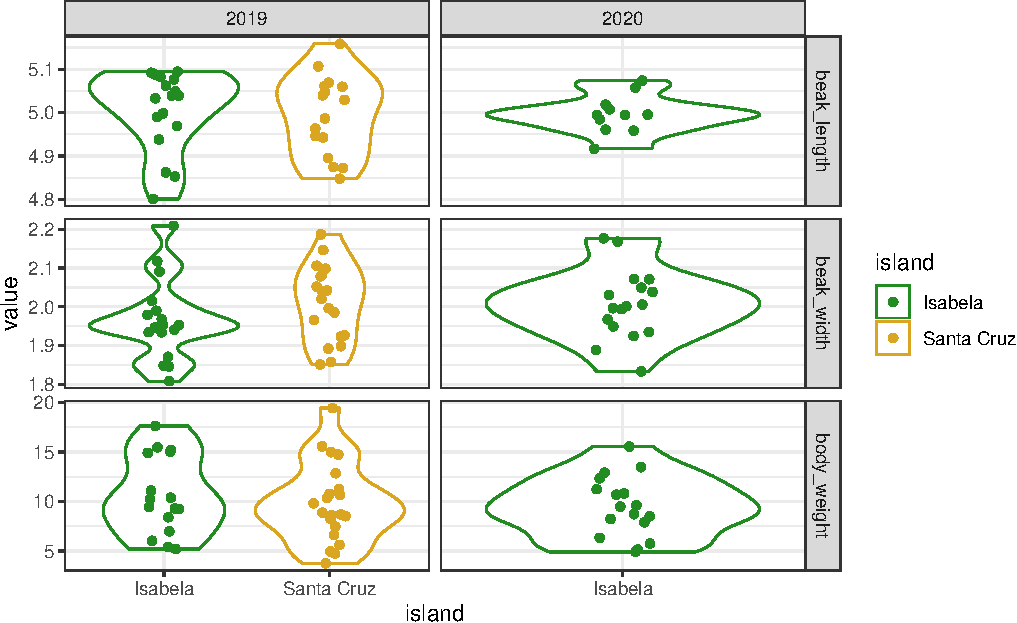
\includegraphics[width=\textwidth]{TRES-Tidy-Tutorial_files/figure-latex/unnamed-chunk-61-1} \end{center}

Here, the islands (horizontal axis) and the variables (the facets) are displayed in alphabetical order. When making a figure you may want to customize these orders in such a way that your message is optimally conveyed by your figure, and this may involve playing with the order of levels.

Use \texttt{fct\_relevel} to manually change the order of the levels:

\begin{Shaded}
\begin{Highlighting}[]
\NormalTok{data}\OperatorTok{$}\NormalTok{island <-}\StringTok{ }\KeywordTok{as.factor}\NormalTok{(data}\OperatorTok{$}\NormalTok{island) }\CommentTok{# turn this column into a factor}
\NormalTok{data}\OperatorTok{$}\NormalTok{island <-}\StringTok{ }\KeywordTok{fct_relevel}\NormalTok{(data}\OperatorTok{$}\NormalTok{island, }\KeywordTok{c}\NormalTok{(}\StringTok{"Santa Cruz"}\NormalTok{, }\StringTok{"Isabela"}\NormalTok{))}
\KeywordTok{my_plot}\NormalTok{(data) }\CommentTok{# order of islands has changed!}
\end{Highlighting}
\end{Shaded}

\begin{center}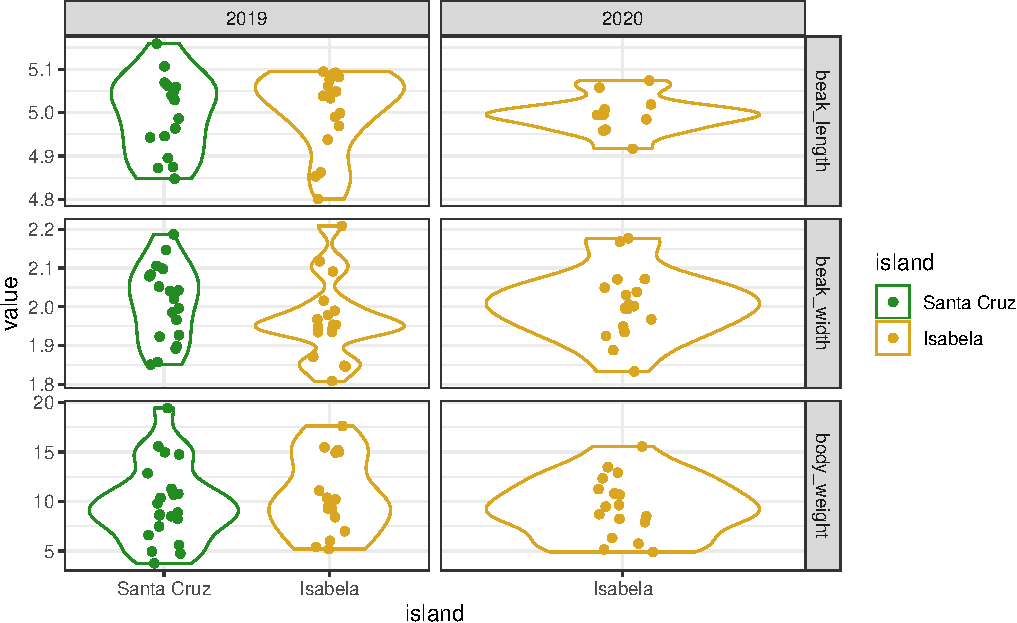
\includegraphics[width=\textwidth]{TRES-Tidy-Tutorial_files/figure-latex/unnamed-chunk-62-1} \end{center}

Beware that reordering a factor \emph{does not change} the order of the items within the vector, only the order of the \emph{levels}. So, it does not introduce any mistmatch between the \texttt{island} column and the other columns! It only matters when the levels are called, for example, in a \texttt{ggplot}. As you can see:

\begin{Shaded}
\begin{Highlighting}[]
\NormalTok{data}\OperatorTok{$}\NormalTok{island[}\DecValTok{1}\OperatorTok{:}\DecValTok{10}\NormalTok{]}
\CommentTok{#>  [1] Isabela Isabela Isabela Isabela Isabela Isabela Isabela Isabela Isabela}
\CommentTok{#> [10] Isabela}
\CommentTok{#> Levels: Santa Cruz Isabela}
\KeywordTok{fct_relevel}\NormalTok{(data}\OperatorTok{$}\NormalTok{island, }\KeywordTok{c}\NormalTok{(}\StringTok{"Isabela"}\NormalTok{, }\StringTok{"Santa Cruz"}\NormalTok{))[}\DecValTok{1}\OperatorTok{:}\DecValTok{10}\NormalTok{] }\CommentTok{# same thing, different levels}
\CommentTok{#>  [1] Isabela Isabela Isabela Isabela Isabela Isabela Isabela Isabela Isabela}
\CommentTok{#> [10] Isabela}
\CommentTok{#> Levels: Isabela Santa Cruz}
\end{Highlighting}
\end{Shaded}

Alternatively, use \texttt{fct\_inorder} to set the order of the levels to the order in which they appear:

\begin{Shaded}
\begin{Highlighting}[]
\NormalTok{data}\OperatorTok{$}\NormalTok{variable <-}\StringTok{ }\KeywordTok{as.factor}\NormalTok{(data}\OperatorTok{$}\NormalTok{variable)}
\KeywordTok{levels}\NormalTok{(data}\OperatorTok{$}\NormalTok{variable)}
\CommentTok{#> [1] "beak_length" "beak_width"  "body_weight"}
\KeywordTok{levels}\NormalTok{(}\KeywordTok{fct_inorder}\NormalTok{(data}\OperatorTok{$}\NormalTok{variable))}
\CommentTok{#> [1] "body_weight" "beak_length" "beak_width"}
\end{Highlighting}
\end{Shaded}

or \texttt{fct\_rev} to reverse the order of the levels:

\begin{Shaded}
\begin{Highlighting}[]
\KeywordTok{levels}\NormalTok{(}\KeywordTok{fct_rev}\NormalTok{(data}\OperatorTok{$}\NormalTok{island)) }\CommentTok{# back in the alphabetical order}
\CommentTok{#> [1] "Isabela"    "Santa Cruz"}
\end{Highlighting}
\end{Shaded}

Other variants exist to do more complex reordering, all present in the forcats \href{https://rstudio.com/resources/cheatsheets/}{cheatsheet}, for example:
* \texttt{fct\_infreq} to re-order according to the frequency of each level (how many observation on each island?)
* \texttt{fct\_shift} to shift the order of all levels by a certain rank (in a circular way so that the last one becomes the first one or vice versa)
* \texttt{fct\_shuffle} if you want your levels in random order
* \texttt{fct\_reorder}, which reorders based on an associated variable (see \texttt{fct\_reorder2} for even more complex relationship between the factor and the associated variable)

\hypertarget{change-the-levels-themselves}{%
\subsection{Change the levels themselves}\label{change-the-levels-themselves}}

Changing the levels of a factor will change the labels in the actual vector. It is similar to performing a string substitution in \texttt{stringr}. One can change the levels of a factor using \texttt{fct\_recode}:

\begin{Shaded}
\begin{Highlighting}[]
\KeywordTok{fct_recode}\NormalTok{(}
\NormalTok{  my_fact_vec, }
  \StringTok{"Pratik Gupte"}\NormalTok{ =}\StringTok{ "Pratik"}\NormalTok{, }
  \StringTok{"Theo Pannetier"}\NormalTok{ =}\StringTok{ "Theo"}\NormalTok{, }
  \StringTok{"Raphael Scherrer"}\NormalTok{ =}\StringTok{ "Raph"}
\NormalTok{)}
\CommentTok{#> [1] Pratik Gupte     Theo Pannetier   Raphael Scherrer}
\CommentTok{#> Levels: Pratik Gupte Raphael Scherrer Theo Pannetier}
\end{Highlighting}
\end{Shaded}

or collapse factor levels together using \texttt{fct\_collapse}:

\begin{Shaded}
\begin{Highlighting}[]
\KeywordTok{fct_collapse}\NormalTok{(my_fact_vec, }\DataTypeTok{EU =} \KeywordTok{c}\NormalTok{(}\StringTok{"Theo"}\NormalTok{, }\StringTok{"Raph"}\NormalTok{), }\DataTypeTok{NonEU =} \StringTok{"Pratik"}\NormalTok{)}
\CommentTok{#> [1] NonEU EU    EU   }
\CommentTok{#> Levels: NonEU EU}
\end{Highlighting}
\end{Shaded}

Again, we do not provide an exhaustive list of \texttt{forcats} functions here but the most usual ones, to give a glimpse of many things that one can do with factors. So, if you are dealing with factors, remember that \texttt{forcats} may have handy tools for you. Among others:
* \texttt{fct\_anon} to ``anonymize'', i.e.~replace the levels by random integers
* \texttt{fct\_lump} to collapse levels together based on their frequency (e.g.~the two most frequent levels together)

\hypertarget{dropping-levels}{%
\subsection{Dropping levels}\label{dropping-levels}}

If you use factors in your tibble and get rid of one level, for any reason, the factor will usually remember the old levels, which may cause some problems when applying functions to your data.

\begin{Shaded}
\begin{Highlighting}[]
\NormalTok{data <-}\StringTok{ }\NormalTok{data[data}\OperatorTok{$}\NormalTok{island }\OperatorTok{==}\StringTok{ "Santa Cruz"}\NormalTok{,] }\CommentTok{# keep only one island}
\KeywordTok{unique}\NormalTok{(data}\OperatorTok{$}\NormalTok{island) }\CommentTok{# Isabela is gone from the labels}
\CommentTok{#> [1] Santa Cruz}
\CommentTok{#> Levels: Santa Cruz Isabela}
\KeywordTok{levels}\NormalTok{(data}\OperatorTok{$}\NormalTok{island) }\CommentTok{# but not from the levels}
\CommentTok{#> [1] "Santa Cruz" "Isabela"}
\end{Highlighting}
\end{Shaded}

Use \texttt{droplevels} (from base R) to make sure you get rid of levels that are not in your data anymore:

\begin{Shaded}
\begin{Highlighting}[]
\NormalTok{data <-}\StringTok{ }\KeywordTok{droplevels}\NormalTok{(data)}
\KeywordTok{levels}\NormalTok{(data}\OperatorTok{$}\NormalTok{island)}
\CommentTok{#> [1] "Santa Cruz"}
\end{Highlighting}
\end{Shaded}

Fortunately, most functions within the tidyverse will not complain about missing levels, and will automatically get rid of those inexistant levels for you. But because factors are such common causes of bugs, keep this in mind!

Note that this is equivalent to doing:

\begin{Shaded}
\begin{Highlighting}[]
\NormalTok{data}\OperatorTok{$}\NormalTok{island <-}\StringTok{ }\KeywordTok{fct_drop}\NormalTok{(data}\OperatorTok{$}\NormalTok{island)}
\end{Highlighting}
\end{Shaded}

\hypertarget{other-things}{%
\subsection{Other things}\label{other-things}}

Among other things you can use in \texttt{forcats}:
* \texttt{fct\_count} to get the frequency of each level
* \texttt{fct\_c} to combine factors together

\hypertarget{take-home-message-for-forcats}{%
\subsection{Take home message for forcats}\label{take-home-message-for-forcats}}

Use this package to manipulate your factors. Do you need factors? Or are character vectors enough? That is your call, and may depend on the kind of analyses you want to do and what they require. We saw here that for plotting, having factors can allow you to do quite some tweaking of the display. If you encounter a situation where the order of encoding of your character vector starts to matter, then maybe converting into a factor would make your life easier. And if you do so, remember that lots of tools to perform all kinds of manipulation are available to you with both \texttt{stringr}and \texttt{forcats}.

\hypertarget{external-resources}{%
\section{External resources}\label{external-resources}}

Find lots of additional info by looking up the following links:

\begin{itemize}
\tightlist
\item
  The \texttt{readr}/\texttt{tibble}/\texttt{tidyr} and \texttt{forcats} \href{https://rstudio.com/resources/cheatsheets/}{cheatsheets}.
\item
  This \href{https://tidyr.tidyverse.org/articles/tidy-data.html}{link} on the concept of tidy data
\item
  The \href{https://tibble.tidyverse.org/}{tibble}, \href{https://tidyr.tidyverse.org/}{tidyr} and \href{https://forcats.tidyverse.org/}{forcats} websites
\item
  The \href{https://broom.tidymodels.org/}{broom}, \href{https://www.tidymodels.org/}{tidymodels}, \href{https://www.data-imaginist.com/2017/introducing-tidygraph/}{tidygraph} and \href{https://yulab-smu.github.io/treedata-book/}{tidytree} websites
\end{itemize}

\hypertarget{data-manipulation-with-dplyr}{%
\chapter{\texorpdfstring{Data manipulation with \texttt{dplyr}}{Data manipulation with dplyr}}\label{data-manipulation-with-dplyr}}

\begin{Shaded}
\begin{Highlighting}[]
\CommentTok{# load the tidyverse}
\KeywordTok{library}\NormalTok{(tidyverse)}
\end{Highlighting}
\end{Shaded}

\hypertarget{introduction}{%
\section{Introduction}\label{introduction}}

\hypertarget{foreword-on-dplyr}{%
\subsection{\texorpdfstring{Foreword on \texttt{dplyr}}{Foreword on dplyr}}\label{foreword-on-dplyr}}

\texttt{dplyr} is tasked with performing all sorts of transformations on a dataset.

The structure of \texttt{dplyr} revolves around a set of functions, the so-called
\textbf{verbs}, that share a common syntax and logic, and are meant to work with one
another in chained operations. Chained operations are performed with the pipe
operator (\texttt{\%\textgreater{}\%}), that will be introduced in section 3.2.2.

The basic syntax is \texttt{verb(data,\ variable)}, where \texttt{data} is a data frame and
\texttt{variable} is the name of one or more columns containing a set of values for
each observation.

There are 5 main verbs, which names already hint at what they do: \texttt{rename()},
\texttt{select()}, \texttt{filter()}, \texttt{mutate()}, and \texttt{summarise()}.
I'm going to introduce each of them (and a couple more) through the following sections.

\hypertarget{example-data}{%
\subsection{Example data}\label{example-data}}

Through this tutorial, we will be using mammal trait data from the \href{https://megapast2future.github.io/PHYLACINE_1.2/}{Phylacine} database.
Let's have a peek at what it contains.

\begin{Shaded}
\begin{Highlighting}[]
\NormalTok{phylacine <-}\StringTok{ }\KeywordTok{read_csv}\NormalTok{(}\StringTok{"data/phylacine_traits.csv"}\NormalTok{)}
\NormalTok{phylacine}
\CommentTok{#> # A tibble: 5,831 x 24}
\CommentTok{#>   Binomial.1.2 Order.1.2 Family.1.2 Genus.1.2 Species.1.2 Terrestrial Marine}
\CommentTok{#>   <chr>        <chr>     <chr>      <chr>     <chr>             <dbl>  <dbl>}
\CommentTok{#> 1 Abditomys_l~ Rodentia  Muridae    Abditomys latidens              1      0}
\CommentTok{#> 2 Abeomelomys~ Rodentia  Muridae    Abeomelo~ sevia                 1      0}
\CommentTok{#> 3 Abrawayaomy~ Rodentia  Cricetidae Abrawaya~ ruschii               1      0}
\CommentTok{#> 4 Abrocoma_be~ Rodentia  Abrocomid~ Abrocoma  bennettii             1      0}
\CommentTok{#> 5 Abrocoma_bo~ Rodentia  Abrocomid~ Abrocoma  boliviensis           1      0}
\CommentTok{#> 6 Abrocoma_bu~ Rodentia  Abrocomid~ Abrocoma  budini                1      0}
\CommentTok{#> # ... with 5,825 more rows, and 17 more variables: Freshwater <dbl>,}
\CommentTok{#> #   Aerial <dbl>, Life.Habit.Method <chr>, Life.Habit.Source <chr>,}
\CommentTok{#> #   Mass.g <dbl>, Mass.Method <chr>, Mass.Source <chr>, Mass.Comparison <chr>,}
\CommentTok{#> #   Mass.Comparison.Source <chr>, Island.Endemicity <chr>,}
\CommentTok{#> #   IUCN.Status.1.2 <chr>, Added.IUCN.Status.1.2 <chr>, Diet.Plant <dbl>,}
\CommentTok{#> #   Diet.Vertebrate <dbl>, Diet.Invertebrate <dbl>, Diet.Method <chr>,}
\CommentTok{#> #   Diet.Source <chr>}
\end{Highlighting}
\end{Shaded}

\texttt{readr} automatically loads the data in a \texttt{tibble}, as we have seen in chapter
1 and 2. Calling the tibble gives a nice preview of what it contains. We have
data for 5,831 mammal species, and the variables contain information on taxonomy,
(broad) habitat, mass, IUCN status, and diet.

If you remember Section 1.2 on tidy data, you may see that this data isn't
exactly tidy. In fact, some columns are in wide (and messy) format, like the
``habitat'' (terrestrial, marine, etc.) and diet columns.

\texttt{dplyr} actually does not require your data to be strictly tidy. If you feel that your
data satisfies the definition ``one observation per row, one variable per column'',
that's probably good enough.

I use a \texttt{tibble} here, but \texttt{dplyr} works equally well on base data frames. In
fact, \texttt{dplyr} is built for \texttt{data.frame} objects, and tibbles are data frames.
Therefore, tibbles are mortal.

\hypertarget{working-with-existing-variables}{%
\section{Working with existing variables}\label{working-with-existing-variables}}

\hypertarget{renaming-variables-with-rename}{%
\subsection{\texorpdfstring{Renaming variables with \texttt{rename()}}{Renaming variables with rename()}}\label{renaming-variables-with-rename}}

The variable names in the phylacine dataset are descriptive, but quite unpractical. Typing
\texttt{Binomial.1.2.} is cumbersome and subject to typos (in fact, I just made one).
\texttt{binomial} would be much simpler to use.

Changing names is straightforward with \texttt{rename()}.

\begin{Shaded}
\begin{Highlighting}[]
\KeywordTok{rename}\NormalTok{(}\DataTypeTok{.data =}\NormalTok{ phylacine, }\StringTok{"binomial"}\NormalTok{ =}\StringTok{ }\NormalTok{Binomial.}\FloatTok{1.2}\NormalTok{)}
\CommentTok{#> # A tibble: 5,831 x 24}
\CommentTok{#>   binomial Order.1.2 Family.1.2 Genus.1.2 Species.1.2 Terrestrial Marine}
\CommentTok{#>   <chr>    <chr>     <chr>      <chr>     <chr>             <dbl>  <dbl>}
\CommentTok{#> 1 Abditom~ Rodentia  Muridae    Abditomys latidens              1      0}
\CommentTok{#> 2 Abeomel~ Rodentia  Muridae    Abeomelo~ sevia                 1      0}
\CommentTok{#> 3 Abraway~ Rodentia  Cricetidae Abrawaya~ ruschii               1      0}
\CommentTok{#> 4 Abrocom~ Rodentia  Abrocomid~ Abrocoma  bennettii             1      0}
\CommentTok{#> 5 Abrocom~ Rodentia  Abrocomid~ Abrocoma  boliviensis           1      0}
\CommentTok{#> 6 Abrocom~ Rodentia  Abrocomid~ Abrocoma  budini                1      0}
\CommentTok{#> # ... with 5,825 more rows, and 17 more variables: Freshwater <dbl>,}
\CommentTok{#> #   Aerial <dbl>, Life.Habit.Method <chr>, Life.Habit.Source <chr>,}
\CommentTok{#> #   Mass.g <dbl>, Mass.Method <chr>, Mass.Source <chr>, Mass.Comparison <chr>,}
\CommentTok{#> #   Mass.Comparison.Source <chr>, Island.Endemicity <chr>,}
\CommentTok{#> #   IUCN.Status.1.2 <chr>, Added.IUCN.Status.1.2 <chr>, Diet.Plant <dbl>,}
\CommentTok{#> #   Diet.Vertebrate <dbl>, Diet.Invertebrate <dbl>, Diet.Method <chr>,}
\CommentTok{#> #   Diet.Source <chr>}
\end{Highlighting}
\end{Shaded}

The first argument is always \texttt{.data}, the data table you want to apply change to.
Note how columns are referred to. Once the data table as been passed as an
argument, there is no need to refer to it directly anymore, \texttt{dplyr} understands
that you're dealing with variables inside that data frame. So drop that
\texttt{data\$var}, \texttt{data{[},\ "var"{]}}, and forget the very existence of \texttt{attach()} /
\texttt{detach()}.

You can refer to variables names either with strings or directly as objects,
whether you're reading or creating them:

\begin{Shaded}
\begin{Highlighting}[]
\KeywordTok{rename}\NormalTok{(}
\NormalTok{  phylacine,}
  \CommentTok{# this works}
  \DataTypeTok{binomial =}\NormalTok{ Binomial.}\FloatTok{1.2}
\NormalTok{)}
\KeywordTok{rename}\NormalTok{(}
\NormalTok{  phylacine,}
  \CommentTok{# this works too!}
  \DataTypeTok{binomial =} \StringTok{"Binomial.1.2"}
\NormalTok{)}
\KeywordTok{rename}\NormalTok{(}
\NormalTok{  phylacine,}
  \CommentTok{# guess what}
  \StringTok{"binomial"}\NormalTok{ =}\StringTok{ "Binomial.1.2"}
\NormalTok{)}
\end{Highlighting}
\end{Shaded}

I have applied similar changes to all variables in the dataset. Here is what the
new names look like:

\begin{verbatim}
#> # A tibble: 5,831 x 24
#>   binomial order family genus species terrestrial marine freshwater aerial
#>   <chr>    <chr> <chr>  <chr> <chr>         <dbl>  <dbl>      <dbl>  <dbl>
#> 1 Abditom~ Rode~ Murid~ Abdi~ latide~           1      0          0      0
#> 2 Abeomel~ Rode~ Murid~ Abeo~ sevia             1      0          0      0
#> 3 Abraway~ Rode~ Crice~ Abra~ ruschii           1      0          0      0
#> 4 Abrocom~ Rode~ Abroc~ Abro~ bennet~           1      0          0      0
#> 5 Abrocom~ Rode~ Abroc~ Abro~ bolivi~           1      0          0      0
#> 6 Abrocom~ Rode~ Abroc~ Abro~ budini            1      0          0      0
#> # ... with 5,825 more rows, and 15 more variables: life_habit_method <chr>,
#> #   life_habit_source <chr>, mass_g <dbl>, mass_method <chr>,
#> #   mass_source <chr>, mass_comparison <chr>, mass_comparison_source <chr>,
#> #   island_endemicity <chr>, iucn_status <chr>, added_iucn_status <chr>,
#> #   diet_plant <dbl>, diet_vertebrate <dbl>, diet_invertebrate <dbl>,
#> #   diet_method <chr>, diet_source <chr>
\end{verbatim}

\hypertarget{the-pipe-operator}{%
\subsection{\texorpdfstring{The pipe operator \texttt{\%\textgreater{}\%}}{The pipe operator \%\textgreater{}\%}}\label{the-pipe-operator}}

If you have already come across pieces of code using the tidyverse, chances are
that you have seen this odd symbol. While the pipe is not strictly-speaking a
part of the tidyverse (it comes from its own package, \texttt{magrittr}), it is
imported along with each package and widely used in conjunction with its
functions.
What does it do? Consider the following example with \texttt{rename()}:

\begin{Shaded}
\begin{Highlighting}[]
\NormalTok{phylacine2 <-}\StringTok{ }\NormalTok{readr}\OperatorTok{::}\KeywordTok{read_csv}\NormalTok{(}\StringTok{"data/phylacine_traits.csv"}\NormalTok{)}
\CommentTok{# regular syntax}
\KeywordTok{rename}\NormalTok{(phylacine2, }\StringTok{"binomial"}\NormalTok{ =}\StringTok{ "Binomial.1.2"}\NormalTok{)}
\CommentTok{#> # A tibble: 5,831 x 24}
\CommentTok{#>   binomial Order.1.2 Family.1.2 Genus.1.2 Species.1.2 Terrestrial Marine}
\CommentTok{#>   <chr>    <chr>     <chr>      <chr>     <chr>             <dbl>  <dbl>}
\CommentTok{#> 1 Abditom~ Rodentia  Muridae    Abditomys latidens              1      0}
\CommentTok{#> 2 Abeomel~ Rodentia  Muridae    Abeomelo~ sevia                 1      0}
\CommentTok{#> 3 Abraway~ Rodentia  Cricetidae Abrawaya~ ruschii               1      0}
\CommentTok{#> 4 Abrocom~ Rodentia  Abrocomid~ Abrocoma  bennettii             1      0}
\CommentTok{#> 5 Abrocom~ Rodentia  Abrocomid~ Abrocoma  boliviensis           1      0}
\CommentTok{#> 6 Abrocom~ Rodentia  Abrocomid~ Abrocoma  budini                1      0}
\CommentTok{#> # ... with 5,825 more rows, and 17 more variables: Freshwater <dbl>,}
\CommentTok{#> #   Aerial <dbl>, Life.Habit.Method <chr>, Life.Habit.Source <chr>,}
\CommentTok{#> #   Mass.g <dbl>, Mass.Method <chr>, Mass.Source <chr>, Mass.Comparison <chr>,}
\CommentTok{#> #   Mass.Comparison.Source <chr>, Island.Endemicity <chr>,}
\CommentTok{#> #   IUCN.Status.1.2 <chr>, Added.IUCN.Status.1.2 <chr>, Diet.Plant <dbl>,}
\CommentTok{#> #   Diet.Vertebrate <dbl>, Diet.Invertebrate <dbl>, Diet.Method <chr>,}
\CommentTok{#> #   Diet.Source <chr>}
\CommentTok{# alternative syntax with the pipe operator}
\NormalTok{phylacine2 }\OperatorTok\StringTok{ }\KeywordTok{rename}\NormalTok{(}\StringTok{"binomial"}\NormalTok{ =}\StringTok{ "Binomial.1.2"}\NormalTok{)}
\CommentTok{#> # A tibble: 5,831 x 24}
\CommentTok{#>   binomial Order.1.2 Family.1.2 Genus.1.2 Species.1.2 Terrestrial Marine}
\CommentTok{#>   <chr>    <chr>     <chr>      <chr>     <chr>             <dbl>  <dbl>}
\CommentTok{#> 1 Abditom~ Rodentia  Muridae    Abditomys latidens              1      0}
\CommentTok{#> 2 Abeomel~ Rodentia  Muridae    Abeomelo~ sevia                 1      0}
\CommentTok{#> 3 Abraway~ Rodentia  Cricetidae Abrawaya~ ruschii               1      0}
\CommentTok{#> 4 Abrocom~ Rodentia  Abrocomid~ Abrocoma  bennettii             1      0}
\CommentTok{#> 5 Abrocom~ Rodentia  Abrocomid~ Abrocoma  boliviensis           1      0}
\CommentTok{#> 6 Abrocom~ Rodentia  Abrocomid~ Abrocoma  budini                1      0}
\CommentTok{#> # ... with 5,825 more rows, and 17 more variables: Freshwater <dbl>,}
\CommentTok{#> #   Aerial <dbl>, Life.Habit.Method <chr>, Life.Habit.Source <chr>,}
\CommentTok{#> #   Mass.g <dbl>, Mass.Method <chr>, Mass.Source <chr>, Mass.Comparison <chr>,}
\CommentTok{#> #   Mass.Comparison.Source <chr>, Island.Endemicity <chr>,}
\CommentTok{#> #   IUCN.Status.1.2 <chr>, Added.IUCN.Status.1.2 <chr>, Diet.Plant <dbl>,}
\CommentTok{#> #   Diet.Vertebrate <dbl>, Diet.Invertebrate <dbl>, Diet.Method <chr>,}
\CommentTok{#> #   Diet.Source <chr>}
\end{Highlighting}
\end{Shaded}

Got it? The pipe takes the object on its left-side and silently feeds it to the
\emph{first} argument of the function on its right-side. It could be read as ``take x,
then do\ldots{}''.
The reason for using the pipe is because it makes code syntax closer to
the syntax of a sentence, and therefore, easier and faster for your brain to
process (and write!) the code. In particular, the pipe enables easy chains of
operations, where you apply something to an object, then apply something else to
the outcome, and so on\ldots{}
Through the later sections, you will see some examples of chained operations
with \texttt{dplyr} functions, but
for that I first need to introduce a couple more verbs.

Using the pipe can be quite unsettling at first, because you are not used to
think in this way. But if you push a bit for it, I promise it will make things
a lot easier (and it's quite addictive!). To avoid typing the tedious symbols,
\texttt{magrittr} installs a shortcut for you in RStudio. Use \texttt{Ctrl\ +\ Shift\ +\ M} on
Windows, and \texttt{Cmd\ +\ Shift\ +\ M} on MacOS.

Finally I should emphasize that the use of the pipe isn't limited to the
tidyverse, but extends to almost all R functions. Remember that by default
the piped value is always matched to the first argument of the following
function

\begin{Shaded}
\begin{Highlighting}[]
\DecValTok{5} \OperatorTok\StringTok{ }\KeywordTok{rep}\NormalTok{(}\DecValTok{3}\NormalTok{)}
\CommentTok{#> [1] 5 5 5}
\StringTok{"meow"} \OperatorTok\StringTok{ }\KeywordTok{cat}\NormalTok{()}
\CommentTok{#> meow}
\end{Highlighting}
\end{Shaded}

If you need to pass the left-hand side to an argument other than the first,
you can use the dot place-holder \texttt{.}.

\begin{Shaded}
\begin{Highlighting}[]
\StringTok{"meow"} \OperatorTok\StringTok{ }\KeywordTok{cat}\NormalTok{(}\StringTok{"cats"}\NormalTok{, }\StringTok{"go"}\NormalTok{)}
\CommentTok{#> meow cats go}
\end{Highlighting}
\end{Shaded}

Because of its syntax, most base R operators are not compatible with the pipe
(but this is very rarely needed).
If needed, \texttt{magrittr} introduces alternative functions for operators.

Subsetting operators can be piped, with the dot place-holder.

\begin{Shaded}
\begin{Highlighting}[]
\CommentTok{# 5 %>% * 3 # no, won't work}
\CommentTok{# 5 %>% .* 3 # neither}
\DecValTok{5} \OperatorTok\StringTok{ }\NormalTok{magrittr}\OperatorTok{::}\KeywordTok{multiply_by}\NormalTok{(}\DecValTok{3}\NormalTok{) }\CommentTok{# yes}
\CommentTok{#> [1] 15}

\CommentTok{# subsetting}
\KeywordTok{list}\NormalTok{(}\StringTok{"monkey see"}\NormalTok{, }\StringTok{"monkey_do"}\NormalTok{) }\OperatorTok\StringTok{ }\NormalTok{.[[}\DecValTok{2}\NormalTok{]]}
\CommentTok{#> [1] "monkey_do"}
\NormalTok{phylacine }\OperatorTok\StringTok{ }\NormalTok{.}\OperatorTok{$}\NormalTok{binomial }\OperatorTok\StringTok{ }\KeywordTok{head}\NormalTok{()}
\CommentTok{#> [1] "Abditomys_latidens"   "Abeomelomys_sevia"    "Abrawayaomys_ruschii"}
\CommentTok{#> [4] "Abrocoma_bennettii"   "Abrocoma_boliviensis" "Abrocoma_budini"}
\end{Highlighting}
\end{Shaded}

Because subsetting in this way is particularly hideous, \texttt{dplyr}
delivers a function to extract values from a single variable. In only works on tables, though.

\begin{Shaded}
\begin{Highlighting}[]
\NormalTok{phylacine }\OperatorTok\StringTok{ }\KeywordTok{pull}\NormalTok{(binomial) }\OperatorTok\StringTok{ }\KeywordTok{head}\NormalTok{()}
\CommentTok{#> [1] "Abditomys_latidens"   "Abeomelomys_sevia"    "Abrawayaomys_ruschii"}
\CommentTok{#> [4] "Abrocoma_bennettii"   "Abrocoma_boliviensis" "Abrocoma_budini"}
\end{Highlighting}
\end{Shaded}

\hypertarget{select-variables-with-select}{%
\subsection{\texorpdfstring{Select variables with \texttt{select()}}{Select variables with select()}}\label{select-variables-with-select}}

To extract a set of variables (i.e.~columns), use the conveniently-named
\texttt{select()}. The basic syntax is the same as \texttt{rename()}: pass your data as the
first argument, then call the variables to select, quoted or not.

\begin{Shaded}
\begin{Highlighting}[]
\CommentTok{# Single variable}
\NormalTok{phylacine }\OperatorTok\StringTok{ }\KeywordTok{select}\NormalTok{(binomial)}
\CommentTok{#> # A tibble: 5,831 x 1}
\CommentTok{#>   binomial            }
\CommentTok{#>   <chr>               }
\CommentTok{#> 1 Abditomys_latidens  }
\CommentTok{#> 2 Abeomelomys_sevia   }
\CommentTok{#> 3 Abrawayaomys_ruschii}
\CommentTok{#> 4 Abrocoma_bennettii  }
\CommentTok{#> 5 Abrocoma_boliviensis}
\CommentTok{#> 6 Abrocoma_budini     }
\CommentTok{#> # ... with 5,825 more rows}
\CommentTok{# A set of variables}
\NormalTok{phylacine }\OperatorTok\StringTok{ }\KeywordTok{select}\NormalTok{(genus, }\StringTok{"species"}\NormalTok{, mass_g)}
\CommentTok{#> # A tibble: 5,831 x 3}
\CommentTok{#>   genus        species     mass_g}
\CommentTok{#>   <chr>        <chr>        <dbl>}
\CommentTok{#> 1 Abditomys    latidens      269 }
\CommentTok{#> 2 Abeomelomys  sevia          52 }
\CommentTok{#> 3 Abrawayaomys ruschii        63 }
\CommentTok{#> 4 Abrocoma     bennettii     250 }
\CommentTok{#> 5 Abrocoma     boliviensis   158 }
\CommentTok{#> 6 Abrocoma     budini        361.}
\CommentTok{#> # ... with 5,825 more rows}
\CommentTok{# A range of contiguous variables}
\NormalTok{phylacine }\OperatorTok\StringTok{ }\KeywordTok{select}\NormalTok{(family}\OperatorTok{:}\NormalTok{terrestrial)}
\CommentTok{#> # A tibble: 5,831 x 4}
\CommentTok{#>   family      genus        species     terrestrial}
\CommentTok{#>   <chr>       <chr>        <chr>             <dbl>}
\CommentTok{#> 1 Muridae     Abditomys    latidens              1}
\CommentTok{#> 2 Muridae     Abeomelomys  sevia                 1}
\CommentTok{#> 3 Cricetidae  Abrawayaomys ruschii               1}
\CommentTok{#> 4 Abrocomidae Abrocoma     bennettii             1}
\CommentTok{#> 5 Abrocomidae Abrocoma     boliviensis           1}
\CommentTok{#> 6 Abrocomidae Abrocoma     budini                1}
\CommentTok{#> # ... with 5,825 more rows}
\end{Highlighting}
\end{Shaded}

You can select by variable numbers. This is not recommended, as prone to
errors, especially if you change the variable order.

\begin{Shaded}
\begin{Highlighting}[]
\NormalTok{phylacine }\OperatorTok\StringTok{ }\KeywordTok{select}\NormalTok{(}\DecValTok{2}\NormalTok{)}
\CommentTok{#> # A tibble: 5,831 x 1}
\CommentTok{#>   order   }
\CommentTok{#>   <chr>   }
\CommentTok{#> 1 Rodentia}
\CommentTok{#> 2 Rodentia}
\CommentTok{#> 3 Rodentia}
\CommentTok{#> 4 Rodentia}
\CommentTok{#> 5 Rodentia}
\CommentTok{#> 6 Rodentia}
\CommentTok{#> # ... with 5,825 more rows}
\end{Highlighting}
\end{Shaded}

\texttt{select()} can also be used to \emph{exclude} variables:

\begin{Shaded}
\begin{Highlighting}[]
\NormalTok{phylacine }\OperatorTok\StringTok{ }\KeywordTok{select}\NormalTok{(}\OperatorTok{-}\NormalTok{binomial)}
\CommentTok{#> # A tibble: 5,831 x 23}
\CommentTok{#>   order family genus species terrestrial marine freshwater aerial}
\CommentTok{#>   <chr> <chr>  <chr> <chr>         <dbl>  <dbl>      <dbl>  <dbl>}
\CommentTok{#> 1 Rode~ Murid~ Abdi~ latide~           1      0          0      0}
\CommentTok{#> 2 Rode~ Murid~ Abeo~ sevia             1      0          0      0}
\CommentTok{#> 3 Rode~ Crice~ Abra~ ruschii           1      0          0      0}
\CommentTok{#> 4 Rode~ Abroc~ Abro~ bennet~           1      0          0      0}
\CommentTok{#> 5 Rode~ Abroc~ Abro~ bolivi~           1      0          0      0}
\CommentTok{#> 6 Rode~ Abroc~ Abro~ budini            1      0          0      0}
\CommentTok{#> # ... with 5,825 more rows, and 15 more variables: life_habit_method <chr>,}
\CommentTok{#> #   life_habit_source <chr>, mass_g <dbl>, mass_method <chr>,}
\CommentTok{#> #   mass_source <chr>, mass_comparison <chr>, mass_comparison_source <chr>,}
\CommentTok{#> #   island_endemicity <chr>, iucn_status <chr>, added_iucn_status <chr>,}
\CommentTok{#> #   diet_plant <dbl>, diet_vertebrate <dbl>, diet_invertebrate <dbl>,}
\CommentTok{#> #   diet_method <chr>, diet_source <chr>}
\NormalTok{phylacine }\OperatorTok\StringTok{ }\KeywordTok{select}\NormalTok{(}\OperatorTok{-}\NormalTok{(binomial}\OperatorTok{:}\NormalTok{species))}
\CommentTok{#> # A tibble: 5,831 x 19}
\CommentTok{#>   terrestrial marine freshwater aerial life_habit_meth~ life_habit_sour~ mass_g}
\CommentTok{#>         <dbl>  <dbl>      <dbl>  <dbl> <chr>            <chr>             <dbl>}
\CommentTok{#> 1           1      0          0      0 Reported         IUCN. 2016. IUC~   269 }
\CommentTok{#> 2           1      0          0      0 Reported         IUCN. 2016. IUC~    52 }
\CommentTok{#> 3           1      0          0      0 Reported         IUCN. 2016. IUC~    63 }
\CommentTok{#> 4           1      0          0      0 Reported         IUCN. 2016. IUC~   250 }
\CommentTok{#> 5           1      0          0      0 Reported         IUCN. 2016. IUC~   158 }
\CommentTok{#> 6           1      0          0      0 Reported         IUCN. 2016. IUC~   361.}
\CommentTok{#> # ... with 5,825 more rows, and 12 more variables: mass_method <chr>,}
\CommentTok{#> #   mass_source <chr>, mass_comparison <chr>, mass_comparison_source <chr>,}
\CommentTok{#> #   island_endemicity <chr>, iucn_status <chr>, added_iucn_status <chr>,}
\CommentTok{#> #   diet_plant <dbl>, diet_vertebrate <dbl>, diet_invertebrate <dbl>,}
\CommentTok{#> #   diet_method <chr>, diet_source <chr>}
\end{Highlighting}
\end{Shaded}

\texttt{select()} and \texttt{rename()} are pretty similar, and in fact, \texttt{select()} can also
rename variables along the way:

\begin{Shaded}
\begin{Highlighting}[]
\NormalTok{phylacine }\OperatorTok\StringTok{ }\KeywordTok{select}\NormalTok{(}\StringTok{"linnaeus"}\NormalTok{ =}\StringTok{ }\NormalTok{binomial)}
\CommentTok{#> # A tibble: 5,831 x 1}
\CommentTok{#>   linnaeus            }
\CommentTok{#>   <chr>               }
\CommentTok{#> 1 Abditomys_latidens  }
\CommentTok{#> 2 Abeomelomys_sevia   }
\CommentTok{#> 3 Abrawayaomys_ruschii}
\CommentTok{#> 4 Abrocoma_bennettii  }
\CommentTok{#> 5 Abrocoma_boliviensis}
\CommentTok{#> 6 Abrocoma_budini     }
\CommentTok{#> # ... with 5,825 more rows}
\end{Highlighting}
\end{Shaded}

And you can mix all of that at once:

\begin{Shaded}
\begin{Highlighting}[]
\NormalTok{phylacine }\OperatorTok\StringTok{ }\KeywordTok{select}\NormalTok{(}
  \StringTok{"fam"}\NormalTok{ =}\StringTok{ }\NormalTok{family,}
\NormalTok{  genus}\OperatorTok{:}\NormalTok{freshwater,}
  \OperatorTok{-}\NormalTok{terrestrial}
\NormalTok{)}
\CommentTok{#> # A tibble: 5,831 x 5}
\CommentTok{#>   fam         genus        species     marine freshwater}
\CommentTok{#>   <chr>       <chr>        <chr>        <dbl>      <dbl>}
\CommentTok{#> 1 Muridae     Abditomys    latidens         0          0}
\CommentTok{#> 2 Muridae     Abeomelomys  sevia            0          0}
\CommentTok{#> 3 Cricetidae  Abrawayaomys ruschii          0          0}
\CommentTok{#> 4 Abrocomidae Abrocoma     bennettii        0          0}
\CommentTok{#> 5 Abrocomidae Abrocoma     boliviensis      0          0}
\CommentTok{#> 6 Abrocomidae Abrocoma     budini           0          0}
\CommentTok{#> # ... with 5,825 more rows}
\end{Highlighting}
\end{Shaded}

\hypertarget{select-variables-with-helpers}{%
\subsection{Select variables with helpers}\label{select-variables-with-helpers}}

The Rstudio team just released \texttt{dplyr\ 1.0.0}, and along with it, some nice
helper functions to ease the selection of a set of variables. I give three
examples here, and encourage you to look at the documentation (\texttt{?select()}) to
find out more.

\begin{Shaded}
\begin{Highlighting}[]
\NormalTok{phylacine }\OperatorTok\StringTok{ }\KeywordTok{select}\NormalTok{(}\KeywordTok{where}\NormalTok{(is.numeric))}
\CommentTok{#> # A tibble: 5,831 x 8}
\CommentTok{#>   terrestrial marine freshwater aerial mass_g diet_plant diet_vertebrate}
\CommentTok{#>         <dbl>  <dbl>      <dbl>  <dbl>  <dbl>      <dbl>           <dbl>}
\CommentTok{#> 1           1      0          0      0   269         100               0}
\CommentTok{#> 2           1      0          0      0    52          78               3}
\CommentTok{#> 3           1      0          0      0    63          88               1}
\CommentTok{#> 4           1      0          0      0   250         100               0}
\CommentTok{#> 5           1      0          0      0   158         100               0}
\CommentTok{#> 6           1      0          0      0   361.        100               0}
\CommentTok{#> # ... with 5,825 more rows, and 1 more variable: diet_invertebrate <dbl>}
\NormalTok{phylacine }\OperatorTok\StringTok{ }\KeywordTok{select}\NormalTok{(}\KeywordTok{contains}\NormalTok{(}\StringTok{"mass"}\NormalTok{) }\OperatorTok{|}\StringTok{ }\KeywordTok{contains}\NormalTok{(}\StringTok{"diet"}\NormalTok{))}
\CommentTok{#> # A tibble: 5,831 x 10}
\CommentTok{#>   mass_g mass_method mass_source mass_comparison mass_comparison~ diet_plant}
\CommentTok{#>    <dbl> <chr>       <chr>       <chr>           <chr>                 <dbl>}
\CommentTok{#> 1   269  Reported    Smith, F. ~ <NA>            <NA>                    100}
\CommentTok{#> 2    52  Reported    Smith, F. ~ <NA>            <NA>                     78}
\CommentTok{#> 3    63  Reported    Smith, F. ~ <NA>            <NA>                     88}
\CommentTok{#> 4   250  Reported    Smith, F. ~ <NA>            <NA>                    100}
\CommentTok{#> 5   158  Reported    Smith, F. ~ <NA>            <NA>                    100}
\CommentTok{#> 6   361. Assumed is~ Journal of~ Abrocoma_ciner~ Journal of Mamm~        100}
\CommentTok{#> # ... with 5,825 more rows, and 4 more variables: diet_vertebrate <dbl>,}
\CommentTok{#> #   diet_invertebrate <dbl>, diet_method <chr>, diet_source <chr>}

\NormalTok{habitats <-}\StringTok{ }\KeywordTok{c}\NormalTok{(}\StringTok{"terrestrial"}\NormalTok{, }\StringTok{"marine"}\NormalTok{, }\StringTok{"arboreal"}\NormalTok{, }\StringTok{"fossorial"}\NormalTok{, }\StringTok{"freshwater"}\NormalTok{)}
\NormalTok{phylacine }\OperatorTok\StringTok{ }\KeywordTok{select}\NormalTok{(}\KeywordTok{any_of}\NormalTok{(habitats))}
\CommentTok{#> # A tibble: 5,831 x 3}
\CommentTok{#>   terrestrial marine freshwater}
\CommentTok{#>         <dbl>  <dbl>      <dbl>}
\CommentTok{#> 1           1      0          0}
\CommentTok{#> 2           1      0          0}
\CommentTok{#> 3           1      0          0}
\CommentTok{#> 4           1      0          0}
\CommentTok{#> 5           1      0          0}
\CommentTok{#> 6           1      0          0}
\CommentTok{#> # ... with 5,825 more rows}
\end{Highlighting}
\end{Shaded}

\hypertarget{rearranging-variable-order-with-relocate}{%
\subsection{\texorpdfstring{Rearranging variable order with \texttt{relocate()}}{Rearranging variable order with relocate()}}\label{rearranging-variable-order-with-relocate}}

The order of variables seldom matters in \texttt{dplyr}, but due to popular demand,
\texttt{dplyr} now has a dedicated verb to rearrange the order of variables. The syntax
is identical to \texttt{rename()}, \texttt{select()}.

\begin{Shaded}
\begin{Highlighting}[]
\NormalTok{phylacine }\OperatorTok\StringTok{ }\KeywordTok{relocate}\NormalTok{(mass_g, }\DataTypeTok{.before =}\NormalTok{ binomial)}
\CommentTok{#> # A tibble: 5,831 x 24}
\CommentTok{#>   mass_g binomial order family genus species terrestrial marine freshwater}
\CommentTok{#>    <dbl> <chr>    <chr> <chr>  <chr> <chr>         <dbl>  <dbl>      <dbl>}
\CommentTok{#> 1   269  Abditom~ Rode~ Murid~ Abdi~ latide~           1      0          0}
\CommentTok{#> 2    52  Abeomel~ Rode~ Murid~ Abeo~ sevia             1      0          0}
\CommentTok{#> 3    63  Abraway~ Rode~ Crice~ Abra~ ruschii           1      0          0}
\CommentTok{#> 4   250  Abrocom~ Rode~ Abroc~ Abro~ bennet~           1      0          0}
\CommentTok{#> 5   158  Abrocom~ Rode~ Abroc~ Abro~ bolivi~           1      0          0}
\CommentTok{#> 6   361. Abrocom~ Rode~ Abroc~ Abro~ budini            1      0          0}
\CommentTok{#> # ... with 5,825 more rows, and 15 more variables: aerial <dbl>,}
\CommentTok{#> #   life_habit_method <chr>, life_habit_source <chr>, mass_method <chr>,}
\CommentTok{#> #   mass_source <chr>, mass_comparison <chr>, mass_comparison_source <chr>,}
\CommentTok{#> #   island_endemicity <chr>, iucn_status <chr>, added_iucn_status <chr>,}
\CommentTok{#> #   diet_plant <dbl>, diet_vertebrate <dbl>, diet_invertebrate <dbl>,}
\CommentTok{#> #   diet_method <chr>, diet_source <chr>}
\NormalTok{phylacine }\OperatorTok\StringTok{ }\KeywordTok{relocate}\NormalTok{(}\KeywordTok{starts_with}\NormalTok{(}\StringTok{"diet"}\NormalTok{), }\DataTypeTok{.after =}\NormalTok{ species)}
\CommentTok{#> # A tibble: 5,831 x 24}
\CommentTok{#>   binomial order family genus species diet_plant diet_vertebrate}
\CommentTok{#>   <chr>    <chr> <chr>  <chr> <chr>        <dbl>           <dbl>}
\CommentTok{#> 1 Abditom~ Rode~ Murid~ Abdi~ latide~        100               0}
\CommentTok{#> 2 Abeomel~ Rode~ Murid~ Abeo~ sevia           78               3}
\CommentTok{#> 3 Abraway~ Rode~ Crice~ Abra~ ruschii         88               1}
\CommentTok{#> 4 Abrocom~ Rode~ Abroc~ Abro~ bennet~        100               0}
\CommentTok{#> 5 Abrocom~ Rode~ Abroc~ Abro~ bolivi~        100               0}
\CommentTok{#> 6 Abrocom~ Rode~ Abroc~ Abro~ budini         100               0}
\CommentTok{#> # ... with 5,825 more rows, and 17 more variables: diet_invertebrate <dbl>,}
\CommentTok{#> #   diet_method <chr>, diet_source <chr>, terrestrial <dbl>, marine <dbl>,}
\CommentTok{#> #   freshwater <dbl>, aerial <dbl>, life_habit_method <chr>,}
\CommentTok{#> #   life_habit_source <chr>, mass_g <dbl>, mass_method <chr>,}
\CommentTok{#> #   mass_source <chr>, mass_comparison <chr>, mass_comparison_source <chr>,}
\CommentTok{#> #   island_endemicity <chr>, iucn_status <chr>, added_iucn_status <chr>}
\end{Highlighting}
\end{Shaded}

\hypertarget{working-with-observations}{%
\section{Working with observations}\label{working-with-observations}}

\hypertarget{ordering-rows-by-value---arrange}{%
\subsection{\texorpdfstring{Ordering rows by value - \texttt{arrange()}}{Ordering rows by value - arrange()}}\label{ordering-rows-by-value---arrange}}

\texttt{arrange()} sorts rows in the data by \textbf{ascending} value for a given variable.
Use the wrapper \texttt{desc()} to sort by descending values instead.

\begin{Shaded}
\begin{Highlighting}[]
\CommentTok{# Smallest mammals}
\NormalTok{phylacine }\OperatorTok\StringTok{ }
\StringTok{  }\KeywordTok{arrange}\NormalTok{(mass_g) }\OperatorTok\StringTok{ }
\StringTok{  }\KeywordTok{select}\NormalTok{(binomial, mass_g)}
\CommentTok{#> # A tibble: 5,831 x 2}
\CommentTok{#>   binomial            mass_g}
\CommentTok{#>   <chr>                <dbl>}
\CommentTok{#> 1 Sorex_yukonicus        1.6}
\CommentTok{#> 2 Crocidura_levicula     1.8}
\CommentTok{#> 3 Suncus_remyi           1.8}
\CommentTok{#> 4 Crocidura_lusitania    2  }
\CommentTok{#> 5 Kerivoula_minuta       2.1}
\CommentTok{#> 6 Suncus_etruscus        2.1}
\CommentTok{#> # ... with 5,825 more rows}

\CommentTok{# Largest mammals}
\NormalTok{phylacine }\OperatorTok\StringTok{ }
\StringTok{  }\KeywordTok{arrange}\NormalTok{(}\KeywordTok{desc}\NormalTok{(mass_g)) }\OperatorTok\StringTok{ }
\StringTok{  }\KeywordTok{select}\NormalTok{(binomial, mass_g)}
\CommentTok{#> # A tibble: 5,831 x 2}
\CommentTok{#>   binomial                  mass_g}
\CommentTok{#>   <chr>                      <dbl>}
\CommentTok{#> 1 Balaenoptera_musculus  190000000}
\CommentTok{#> 2 Balaena_mysticetus     100000000}
\CommentTok{#> 3 Balaenoptera_physalus   70000000}
\CommentTok{#> 4 Caperea_marginata       32000000}
\CommentTok{#> 5 Megaptera_novaeangliae  30000000}
\CommentTok{#> 6 Eschrichtius_robustus   28500000}
\CommentTok{#> # ... with 5,825 more rows}

\CommentTok{# Extra variables are used to sort ties in the first variable}
\NormalTok{phylacine }\OperatorTok\StringTok{ }
\StringTok{  }\KeywordTok{arrange}\NormalTok{(mass_g, }\KeywordTok{desc}\NormalTok{(binomial)) }\OperatorTok\StringTok{ }
\StringTok{  }\KeywordTok{select}\NormalTok{(binomial, mass_g)}
\CommentTok{#> # A tibble: 5,831 x 2}
\CommentTok{#>   binomial            mass_g}
\CommentTok{#>   <chr>                <dbl>}
\CommentTok{#> 1 Sorex_yukonicus        1.6}
\CommentTok{#> 2 Suncus_remyi           1.8}
\CommentTok{#> 3 Crocidura_levicula     1.8}
\CommentTok{#> 4 Crocidura_lusitania    2  }
\CommentTok{#> 5 Suncus_etruscus        2.1}
\CommentTok{#> 6 Kerivoula_minuta       2.1}
\CommentTok{#> # ... with 5,825 more rows}
\end{Highlighting}
\end{Shaded}

\emph{Important}: \texttt{NA} values, if present, are always ordered at the end!

\hypertarget{subset-rows-by-position---slice}{%
\subsection{\texorpdfstring{Subset rows by position - \texttt{slice()}}{Subset rows by position - slice()}}\label{subset-rows-by-position---slice}}

Use \texttt{slice()} and its variants to extract particular rows.

\begin{Shaded}
\begin{Highlighting}[]
\NormalTok{phylacine }\OperatorTok\StringTok{ }\KeywordTok{slice}\NormalTok{(}\DecValTok{3}\NormalTok{) }\CommentTok{# third row}
\CommentTok{#> # A tibble: 1 x 24}
\CommentTok{#>   binomial order family genus species terrestrial marine freshwater aerial}
\CommentTok{#>   <chr>    <chr> <chr>  <chr> <chr>         <dbl>  <dbl>      <dbl>  <dbl>}
\CommentTok{#> 1 Abraway~ Rode~ Crice~ Abra~ ruschii           1      0          0      0}
\CommentTok{#> # ... with 15 more variables: life_habit_method <chr>, life_habit_source <chr>,}
\CommentTok{#> #   mass_g <dbl>, mass_method <chr>, mass_source <chr>, mass_comparison <chr>,}
\CommentTok{#> #   mass_comparison_source <chr>, island_endemicity <chr>, iucn_status <chr>,}
\CommentTok{#> #   added_iucn_status <chr>, diet_plant <dbl>, diet_vertebrate <dbl>,}
\CommentTok{#> #   diet_invertebrate <dbl>, diet_method <chr>, diet_source <chr>}
\NormalTok{phylacine }\OperatorTok\StringTok{ }\KeywordTok{slice}\NormalTok{(}\DecValTok{5}\NormalTok{, }\DecValTok{1}\NormalTok{, }\DecValTok{2}\NormalTok{) }\CommentTok{# fifth, first and second row}
\CommentTok{#> # A tibble: 3 x 24}
\CommentTok{#>   binomial order family genus species terrestrial marine freshwater aerial}
\CommentTok{#>   <chr>    <chr> <chr>  <chr> <chr>         <dbl>  <dbl>      <dbl>  <dbl>}
\CommentTok{#> 1 Abrocom~ Rode~ Abroc~ Abro~ bolivi~           1      0          0      0}
\CommentTok{#> 2 Abditom~ Rode~ Murid~ Abdi~ latide~           1      0          0      0}
\CommentTok{#> 3 Abeomel~ Rode~ Murid~ Abeo~ sevia             1      0          0      0}
\CommentTok{#> # ... with 15 more variables: life_habit_method <chr>, life_habit_source <chr>,}
\CommentTok{#> #   mass_g <dbl>, mass_method <chr>, mass_source <chr>, mass_comparison <chr>,}
\CommentTok{#> #   mass_comparison_source <chr>, island_endemicity <chr>, iucn_status <chr>,}
\CommentTok{#> #   added_iucn_status <chr>, diet_plant <dbl>, diet_vertebrate <dbl>,}
\CommentTok{#> #   diet_invertebrate <dbl>, diet_method <chr>, diet_source <chr>}
\NormalTok{phylacine }\OperatorTok\StringTok{ }\KeywordTok{slice}\NormalTok{(}\KeywordTok{rep}\NormalTok{(}\DecValTok{3}\NormalTok{, }\DecValTok{2}\NormalTok{)) }\CommentTok{# duplicate the third row}
\CommentTok{#> # A tibble: 2 x 24}
\CommentTok{#>   binomial order family genus species terrestrial marine freshwater aerial}
\CommentTok{#>   <chr>    <chr> <chr>  <chr> <chr>         <dbl>  <dbl>      <dbl>  <dbl>}
\CommentTok{#> 1 Abraway~ Rode~ Crice~ Abra~ ruschii           1      0          0      0}
\CommentTok{#> 2 Abraway~ Rode~ Crice~ Abra~ ruschii           1      0          0      0}
\CommentTok{#> # ... with 15 more variables: life_habit_method <chr>, life_habit_source <chr>,}
\CommentTok{#> #   mass_g <dbl>, mass_method <chr>, mass_source <chr>, mass_comparison <chr>,}
\CommentTok{#> #   mass_comparison_source <chr>, island_endemicity <chr>, iucn_status <chr>,}
\CommentTok{#> #   added_iucn_status <chr>, diet_plant <dbl>, diet_vertebrate <dbl>,}
\CommentTok{#> #   diet_invertebrate <dbl>, diet_method <chr>, diet_source <chr>}
\NormalTok{phylacine }\OperatorTok\StringTok{ }\KeywordTok{slice}\NormalTok{(}\OperatorTok{-}\KeywordTok{c}\NormalTok{(}\DecValTok{2}\OperatorTok{:}\DecValTok{5830}\NormalTok{)) }\CommentTok{# exclude all but first and last row}
\CommentTok{#> # A tibble: 2 x 24}
\CommentTok{#>   binomial order family genus species terrestrial marine freshwater aerial}
\CommentTok{#>   <chr>    <chr> <chr>  <chr> <chr>         <dbl>  <dbl>      <dbl>  <dbl>}
\CommentTok{#> 1 Abditom~ Rode~ Murid~ Abdi~ latide~           1      0          0      0}
\CommentTok{#> 2 Zyzomys~ Rode~ Murid~ Zyzo~ woodwa~           1      0          0      0}
\CommentTok{#> # ... with 15 more variables: life_habit_method <chr>, life_habit_source <chr>,}
\CommentTok{#> #   mass_g <dbl>, mass_method <chr>, mass_source <chr>, mass_comparison <chr>,}
\CommentTok{#> #   mass_comparison_source <chr>, island_endemicity <chr>, iucn_status <chr>,}
\CommentTok{#> #   added_iucn_status <chr>, diet_plant <dbl>, diet_vertebrate <dbl>,}
\CommentTok{#> #   diet_invertebrate <dbl>, diet_method <chr>, diet_source <chr>}

\NormalTok{phylacine }\OperatorTok\StringTok{ }\KeywordTok{slice_tail}\NormalTok{(}\DataTypeTok{n =} \DecValTok{3}\NormalTok{) }\CommentTok{# last three rows}
\CommentTok{#> # A tibble: 3 x 24}
\CommentTok{#>   binomial order family genus species terrestrial marine freshwater aerial}
\CommentTok{#>   <chr>    <chr> <chr>  <chr> <chr>         <dbl>  <dbl>      <dbl>  <dbl>}
\CommentTok{#> 1 Zyzomys~ Rode~ Murid~ Zyzo~ palata~           1      0          0      0}
\CommentTok{#> 2 Zyzomys~ Rode~ Murid~ Zyzo~ pedunc~           1      0          0      0}
\CommentTok{#> 3 Zyzomys~ Rode~ Murid~ Zyzo~ woodwa~           1      0          0      0}
\CommentTok{#> # ... with 15 more variables: life_habit_method <chr>, life_habit_source <chr>,}
\CommentTok{#> #   mass_g <dbl>, mass_method <chr>, mass_source <chr>, mass_comparison <chr>,}
\CommentTok{#> #   mass_comparison_source <chr>, island_endemicity <chr>, iucn_status <chr>,}
\CommentTok{#> #   added_iucn_status <chr>, diet_plant <dbl>, diet_vertebrate <dbl>,}
\CommentTok{#> #   diet_invertebrate <dbl>, diet_method <chr>, diet_source <chr>}
\NormalTok{phylacine }\OperatorTok\StringTok{ }\KeywordTok{slice_max}\NormalTok{(mass_g) }\CommentTok{# largest mammal}
\CommentTok{#> # A tibble: 1 x 24}
\CommentTok{#>   binomial order family genus species terrestrial marine freshwater aerial}
\CommentTok{#>   <chr>    <chr> <chr>  <chr> <chr>         <dbl>  <dbl>      <dbl>  <dbl>}
\CommentTok{#> 1 Balaeno~ Ceta~ Balae~ Bala~ muscul~           0      1          0      0}
\CommentTok{#> # ... with 15 more variables: life_habit_method <chr>, life_habit_source <chr>,}
\CommentTok{#> #   mass_g <dbl>, mass_method <chr>, mass_source <chr>, mass_comparison <chr>,}
\CommentTok{#> #   mass_comparison_source <chr>, island_endemicity <chr>, iucn_status <chr>,}
\CommentTok{#> #   added_iucn_status <chr>, diet_plant <dbl>, diet_vertebrate <dbl>,}
\CommentTok{#> #   diet_invertebrate <dbl>, diet_method <chr>, diet_source <chr>}
\end{Highlighting}
\end{Shaded}

You can also sample random rows in the data:

\begin{Shaded}
\begin{Highlighting}[]
\NormalTok{phylacine }\OperatorTok\StringTok{ }\KeywordTok{slice_sample}\NormalTok{() }\CommentTok{# a random row}
\CommentTok{#> # A tibble: 1 x 24}
\CommentTok{#>   binomial order family genus species terrestrial marine freshwater aerial}
\CommentTok{#>   <chr>    <chr> <chr>  <chr> <chr>         <dbl>  <dbl>      <dbl>  <dbl>}
\CommentTok{#> 1 Crocidu~ Euli~ Soric~ Croc~ levicu~           1      0          0      0}
\CommentTok{#> # ... with 15 more variables: life_habit_method <chr>, life_habit_source <chr>,}
\CommentTok{#> #   mass_g <dbl>, mass_method <chr>, mass_source <chr>, mass_comparison <chr>,}
\CommentTok{#> #   mass_comparison_source <chr>, island_endemicity <chr>, iucn_status <chr>,}
\CommentTok{#> #   added_iucn_status <chr>, diet_plant <dbl>, diet_vertebrate <dbl>,}
\CommentTok{#> #   diet_invertebrate <dbl>, diet_method <chr>, diet_source <chr>}

\CommentTok{# bootstrap}
\NormalTok{phylacine }\OperatorTok\StringTok{ }\KeywordTok{slice_sample}\NormalTok{(}\DataTypeTok{n =} \DecValTok{5831}\NormalTok{, }\DataTypeTok{replace =} \OtherTok{TRUE}\NormalTok{)}
\CommentTok{#> # A tibble: 5,831 x 24}
\CommentTok{#>   binomial order family genus species terrestrial marine freshwater aerial}
\CommentTok{#>   <chr>    <chr> <chr>  <chr> <chr>         <dbl>  <dbl>      <dbl>  <dbl>}
\CommentTok{#> 1 Rhinolo~ Chir~ Rhino~ Rhin~ adami             0      0          0      1}
\CommentTok{#> 2 Hylomys~ Euli~ Erina~ Hylo~ megalo~           1      0          0      0}
\CommentTok{#> 3 Sciurus~ Rode~ Sciur~ Sciu~ yucata~           1      0          0      0}
\CommentTok{#> 4 Emballo~ Chir~ Embal~ Emba~ alecto            0      0          0      1}
\CommentTok{#> 5 Pteralo~ Chir~ Ptero~ Pter~ taki              0      0          0      1}
\CommentTok{#> 6 Lasiorh~ Dipr~ Vomba~ Lasi~ latifr~           1      0          0      0}
\CommentTok{#> # ... with 5,825 more rows, and 15 more variables: life_habit_method <chr>,}
\CommentTok{#> #   life_habit_source <chr>, mass_g <dbl>, mass_method <chr>,}
\CommentTok{#> #   mass_source <chr>, mass_comparison <chr>, mass_comparison_source <chr>,}
\CommentTok{#> #   island_endemicity <chr>, iucn_status <chr>, added_iucn_status <chr>,}
\CommentTok{#> #   diet_plant <dbl>, diet_vertebrate <dbl>, diet_invertebrate <dbl>,}
\CommentTok{#> #   diet_method <chr>, diet_source <chr>}
\end{Highlighting}
\end{Shaded}

\hypertarget{subsetting-rows-by-value-with-filter}{%
\subsection{\texorpdfstring{Subsetting rows by value with \texttt{filter()}}{Subsetting rows by value with filter()}}\label{subsetting-rows-by-value-with-filter}}

\texttt{filter()} does a similar job as \texttt{slice()}, but extract rows that satisfy a set
of conditions. The conditions are supplied much the same way as you would do
for an \texttt{if} statement.

Along with \texttt{mutate()} (next section), this is probably the function you are
going to use the most.

For example, I might want to extract mammals above a given mass:

\begin{Shaded}
\begin{Highlighting}[]
\CommentTok{# megafauna}
\NormalTok{phylacine }\OperatorTok\StringTok{ }
\StringTok{  }\KeywordTok{filter}\NormalTok{(mass_g }\OperatorTok{>}\StringTok{ }\FloatTok{1e5}\NormalTok{) }\OperatorTok\StringTok{ }\CommentTok{# 100 kg}
\StringTok{  }\KeywordTok{select}\NormalTok{(binomial, mass_g)}
\CommentTok{#> # A tibble: 302 x 2}
\CommentTok{#>   binomial                   mass_g}
\CommentTok{#>   <chr>                       <dbl>}
\CommentTok{#> 1 Ailuropoda_melanoleuca    108400 }
\CommentTok{#> 2 Alcelaphus_buselaphus     171002.}
\CommentTok{#> 3 Alces_alces               356998 }
\CommentTok{#> 4 Archaeoindris_fontoynonti 160000 }
\CommentTok{#> 5 Arctocephalus_forsteri    101250 }
\CommentTok{#> 6 Arctocephalus_pusillus    178500 }
\CommentTok{#> # ... with 296 more rows}

\CommentTok{# non-extinct megafauna}
\NormalTok{phylacine }\OperatorTok\StringTok{ }
\StringTok{  }\KeywordTok{filter}\NormalTok{(mass_g }\OperatorTok{>}\StringTok{ }\FloatTok{1e5}\NormalTok{, iucn_status }\OperatorTok{!=}\StringTok{ "EP"}\NormalTok{) }\OperatorTok\StringTok{ }
\StringTok{  }\KeywordTok{select}\NormalTok{(binomial, mass_g, iucn_status)}
\CommentTok{#> # A tibble: 178 x 3}
\CommentTok{#>   binomial                 mass_g iucn_status}
\CommentTok{#>   <chr>                     <dbl> <chr>      }
\CommentTok{#> 1 Ailuropoda_melanoleuca  108400  VU         }
\CommentTok{#> 2 Alcelaphus_buselaphus   171002. LC         }
\CommentTok{#> 3 Alces_alces             356998  LC         }
\CommentTok{#> 4 Arctocephalus_forsteri  101250  LC         }
\CommentTok{#> 5 Arctocephalus_pusillus  178500  LC         }
\CommentTok{#> 6 Arctocephalus_townsendi 105000  LC         }
\CommentTok{#> # ... with 172 more rows}
\end{Highlighting}
\end{Shaded}

Are there any flying mammals that aren't bats?

\begin{Shaded}
\begin{Highlighting}[]
\NormalTok{phylacine }\OperatorTok\StringTok{ }
\StringTok{  }\KeywordTok{filter}\NormalTok{(aerial }\OperatorTok{==}\StringTok{ }\DecValTok{1}\NormalTok{, order }\OperatorTok{!=}\StringTok{ "Chiroptera"}\NormalTok{) }
\CommentTok{#> # A tibble: 0 x 24}
\CommentTok{#> # ... with 24 variables: binomial <chr>, order <chr>, family <chr>,}
\CommentTok{#> #   genus <chr>, species <chr>, terrestrial <dbl>, marine <dbl>,}
\CommentTok{#> #   freshwater <dbl>, aerial <dbl>, life_habit_method <chr>,}
\CommentTok{#> #   life_habit_source <chr>, mass_g <dbl>, mass_method <chr>,}
\CommentTok{#> #   mass_source <chr>, mass_comparison <chr>, mass_comparison_source <chr>,}
\CommentTok{#> #   island_endemicity <chr>, iucn_status <chr>, added_iucn_status <chr>,}
\CommentTok{#> #   diet_plant <dbl>, diet_vertebrate <dbl>, diet_invertebrate <dbl>,}
\CommentTok{#> #   diet_method <chr>, diet_source <chr>}
\CommentTok{# no :(}
\end{Highlighting}
\end{Shaded}

Are humans included in the table?

\begin{Shaded}
\begin{Highlighting}[]
\NormalTok{phylacine }\OperatorTok\StringTok{ }\KeywordTok{filter}\NormalTok{(binomial }\OperatorTok{==}\StringTok{ "Homo_sapiens"}\NormalTok{)}
\CommentTok{#> # A tibble: 1 x 24}
\CommentTok{#>   binomial order family genus species terrestrial marine freshwater aerial}
\CommentTok{#>   <chr>    <chr> <chr>  <chr> <chr>         <dbl>  <dbl>      <dbl>  <dbl>}
\CommentTok{#> 1 Homo_sa~ Prim~ Homin~ Homo  sapiens           1      0          0      0}
\CommentTok{#> # ... with 15 more variables: life_habit_method <chr>, life_habit_source <chr>,}
\CommentTok{#> #   mass_g <dbl>, mass_method <chr>, mass_source <chr>, mass_comparison <chr>,}
\CommentTok{#> #   mass_comparison_source <chr>, island_endemicity <chr>, iucn_status <chr>,}
\CommentTok{#> #   added_iucn_status <chr>, diet_plant <dbl>, diet_vertebrate <dbl>,}
\CommentTok{#> #   diet_invertebrate <dbl>, diet_method <chr>, diet_source <chr>}
\end{Highlighting}
\end{Shaded}

\texttt{filter()} can be used to deal with NAs:

\begin{Shaded}
\begin{Highlighting}[]
\NormalTok{phylacine }\OperatorTok\StringTok{ }
\StringTok{  }\KeywordTok{filter}\NormalTok{(}\OperatorTok{!}\KeywordTok{is.na}\NormalTok{(mass_comparison)) }
\CommentTok{#> # A tibble: 754 x 24}
\CommentTok{#>   binomial order family genus species terrestrial marine freshwater aerial}
\CommentTok{#>   <chr>    <chr> <chr>  <chr> <chr>         <dbl>  <dbl>      <dbl>  <dbl>}
\CommentTok{#> 1 Abrocom~ Rode~ Abroc~ Abro~ budini            1      0          0      0}
\CommentTok{#> 2 Abrocom~ Rode~ Abroc~ Abro~ famati~           1      0          0      0}
\CommentTok{#> 3 Abrocom~ Rode~ Abroc~ Abro~ shista~           1      0          0      0}
\CommentTok{#> 4 Abrocom~ Rode~ Abroc~ Abro~ uspall~           1      0          0      0}
\CommentTok{#> 5 Abrocom~ Rode~ Abroc~ Abro~ vaccar~           1      0          0      0}
\CommentTok{#> 6 Acerodo~ Chir~ Ptero~ Acer~ humilis           0      0          0      1}
\CommentTok{#> # ... with 748 more rows, and 15 more variables: life_habit_method <chr>,}
\CommentTok{#> #   life_habit_source <chr>, mass_g <dbl>, mass_method <chr>,}
\CommentTok{#> #   mass_source <chr>, mass_comparison <chr>, mass_comparison_source <chr>,}
\CommentTok{#> #   island_endemicity <chr>, iucn_status <chr>, added_iucn_status <chr>,}
\CommentTok{#> #   diet_plant <dbl>, diet_vertebrate <dbl>, diet_invertebrate <dbl>,}
\CommentTok{#> #   diet_method <chr>, diet_source <chr>}
\end{Highlighting}
\end{Shaded}

Tip: \texttt{dplyr} introduces the useful function \texttt{between()} that does exactly what the name implies

\begin{Shaded}
\begin{Highlighting}[]
\KeywordTok{between}\NormalTok{(}\DecValTok{1}\OperatorTok{:}\DecValTok{5}\NormalTok{, }\DecValTok{2}\NormalTok{, }\DecValTok{4}\NormalTok{)}
\CommentTok{#> [1] FALSE  TRUE  TRUE  TRUE FALSE}

\CommentTok{# Mesofauna}
\NormalTok{phylacine }\OperatorTok\StringTok{ }
\StringTok{  }\KeywordTok{filter}\NormalTok{(mass_g }\OperatorTok{>}\StringTok{ }\FloatTok{1e3}\NormalTok{, mass_g }\OperatorTok{<}\StringTok{ }\FloatTok{1e5}\NormalTok{) }\OperatorTok\StringTok{ }
\StringTok{  }\KeywordTok{select}\NormalTok{(binomial, mass_g)}
\CommentTok{#> # A tibble: 1,126 x 2}
\CommentTok{#>   binomial                mass_g}
\CommentTok{#>   <chr>                    <dbl>}
\CommentTok{#> 1 Acerodon_jubatus         1075 }
\CommentTok{#> 2 Acinonyx_jubatus        46700 }
\CommentTok{#> 3 Acratocnus_odontrigonus 22990 }
\CommentTok{#> 4 Acratocnus_ye           21310 }
\CommentTok{#> 5 Addax_nasomaculatus     70000.}
\CommentTok{#> 6 Aepyceros_melampus      52500.}
\CommentTok{#> # ... with 1,120 more rows}

\CommentTok{# same thing}
\NormalTok{phylacine }\OperatorTok\StringTok{ }
\StringTok{  }\KeywordTok{filter}\NormalTok{(mass_g }\OperatorTok\StringTok{ }\KeywordTok{between}\NormalTok{(}\FloatTok{1e3}\NormalTok{, }\FloatTok{1e5}\NormalTok{)) }\OperatorTok\StringTok{ }
\StringTok{  }\KeywordTok{select}\NormalTok{(binomial, mass_g)}
\CommentTok{#> # A tibble: 1,148 x 2}
\CommentTok{#>   binomial                mass_g}
\CommentTok{#>   <chr>                    <dbl>}
\CommentTok{#> 1 Acerodon_jubatus         1075 }
\CommentTok{#> 2 Acinonyx_jubatus        46700 }
\CommentTok{#> 3 Acratocnus_odontrigonus 22990 }
\CommentTok{#> 4 Acratocnus_ye           21310 }
\CommentTok{#> 5 Addax_nasomaculatus     70000.}
\CommentTok{#> 6 Aepyceros_melampus      52500.}
\CommentTok{#> # ... with 1,142 more rows}
\end{Highlighting}
\end{Shaded}

Note that you can pipe operations inside function arguments as in the last line
above (arguments are expressions, after all!).

\hypertarget{making-new-variables}{%
\section{Making new variables}\label{making-new-variables}}

\hypertarget{create-new-variables-with-mutate}{%
\subsection{\texorpdfstring{Create new variables with \texttt{mutate()}}{Create new variables with mutate()}}\label{create-new-variables-with-mutate}}

Very often in data analysis, you will want to create new variables, or edit
existing ones. This is done easily through \texttt{mutate()}. For example, consider
the diet data:

\begin{Shaded}
\begin{Highlighting}[]
\NormalTok{diet <-}\StringTok{ }\NormalTok{phylacine }\OperatorTok\StringTok{ }
\StringTok{  }\KeywordTok{select}\NormalTok{(}
\NormalTok{    binomial,}
    \KeywordTok{contains}\NormalTok{(}\StringTok{"diet"}\NormalTok{) }\OperatorTok{&}\StringTok{ }\OperatorTok{!}\KeywordTok{contains}\NormalTok{(}\KeywordTok{c}\NormalTok{(}\StringTok{"method"}\NormalTok{, }\StringTok{"source"}\NormalTok{))}
\NormalTok{  )}
\NormalTok{diet}
\CommentTok{#> # A tibble: 5,831 x 4}
\CommentTok{#>   binomial             diet_plant diet_vertebrate diet_invertebrate}
\CommentTok{#>   <chr>                     <dbl>           <dbl>             <dbl>}
\CommentTok{#> 1 Abditomys_latidens          100               0                 0}
\CommentTok{#> 2 Abeomelomys_sevia            78               3                19}
\CommentTok{#> 3 Abrawayaomys_ruschii         88               1                11}
\CommentTok{#> 4 Abrocoma_bennettii          100               0                 0}
\CommentTok{#> 5 Abrocoma_boliviensis        100               0                 0}
\CommentTok{#> 6 Abrocoma_budini             100               0                 0}
\CommentTok{#> # ... with 5,825 more rows}
\end{Highlighting}
\end{Shaded}

These three variables show the percentage of each category of food that make the
diet of that species. They should sum to 100, unless the authors made a typo or
other entry error. To assert this, I'm going to create a new variable,
\texttt{total\_diet}.

\begin{Shaded}
\begin{Highlighting}[]
\NormalTok{diet <-}\StringTok{ }\NormalTok{diet }\OperatorTok\StringTok{ }\KeywordTok{mutate}\NormalTok{(}
  \StringTok{"total_diet"}\NormalTok{ =}\StringTok{ }\NormalTok{diet_vertebrate }\OperatorTok{+}\StringTok{ }\NormalTok{diet_invertebrate }\OperatorTok{+}\StringTok{ }\NormalTok{diet_plant}
\NormalTok{)}
\NormalTok{diet}
\CommentTok{#> # A tibble: 5,831 x 5}
\CommentTok{#>   binomial             diet_plant diet_vertebrate diet_invertebrate total_diet}
\CommentTok{#>   <chr>                     <dbl>           <dbl>             <dbl>      <dbl>}
\CommentTok{#> 1 Abditomys_latidens          100               0                 0        100}
\CommentTok{#> 2 Abeomelomys_sevia            78               3                19        100}
\CommentTok{#> 3 Abrawayaomys_ruschii         88               1                11        100}
\CommentTok{#> 4 Abrocoma_bennettii          100               0                 0        100}
\CommentTok{#> 5 Abrocoma_boliviensis        100               0                 0        100}
\CommentTok{#> 6 Abrocoma_budini             100               0                 0        100}
\CommentTok{#> # ... with 5,825 more rows}

\KeywordTok{all}\NormalTok{(diet}\OperatorTok{$}\NormalTok{total_diet }\OperatorTok{==}\StringTok{ }\DecValTok{100}\NormalTok{)}
\CommentTok{#> [1] TRUE}
\CommentTok{# cool and good}
\end{Highlighting}
\end{Shaded}

\texttt{mutate()} adds a variable to the table, and keeps all other variables.
Sometimes you may want to just keep the new variable, and drop the other ones.
That's the job of \texttt{mutate()}'s twin sibling, \texttt{transmute()}. For example,
I want to combine \texttt{diet\_invertebrate} and \texttt{diet\_vertebrate} together:

\begin{Shaded}
\begin{Highlighting}[]
\NormalTok{diet }\OperatorTok\StringTok{ }
\StringTok{  }\KeywordTok{transmute}\NormalTok{(}
    \StringTok{"diet_animal"}\NormalTok{ =}\StringTok{ }\NormalTok{diet_invertebrate }\OperatorTok{+}\StringTok{ }\NormalTok{diet_vertebrate}
\NormalTok{  )}
\CommentTok{#> # A tibble: 5,831 x 1}
\CommentTok{#>   diet_animal}
\CommentTok{#>         <dbl>}
\CommentTok{#> 1           0}
\CommentTok{#> 2          22}
\CommentTok{#> 3          12}
\CommentTok{#> 4           0}
\CommentTok{#> 5           0}
\CommentTok{#> 6           0}
\CommentTok{#> # ... with 5,825 more rows}
\end{Highlighting}
\end{Shaded}

You may want to keep some variables and drop others. You could pipe \texttt{mutate()}
and \texttt{select()} to do so, or you could just pass the variables to keep to
\texttt{transmute()}.

\begin{Shaded}
\begin{Highlighting}[]
\NormalTok{diet }\OperatorTok\StringTok{ }
\StringTok{  }\KeywordTok{transmute}\NormalTok{(}
    \StringTok{"diet_animal"}\NormalTok{ =}\StringTok{ }\NormalTok{diet_invertebrate }\OperatorTok{+}\StringTok{ }\NormalTok{diet_vertebrate,}
\NormalTok{    diet_plant}
\NormalTok{  )}
\CommentTok{#> # A tibble: 5,831 x 2}
\CommentTok{#>   diet_animal diet_plant}
\CommentTok{#>         <dbl>      <dbl>}
\CommentTok{#> 1           0        100}
\CommentTok{#> 2          22         78}
\CommentTok{#> 3          12         88}
\CommentTok{#> 4           0        100}
\CommentTok{#> 5           0        100}
\CommentTok{#> 6           0        100}
\CommentTok{#> # ... with 5,825 more rows}
\end{Highlighting}
\end{Shaded}

You can also refer to variables you're creating to derive new variables from
them as part of the same operation, this is not an issue.

\begin{Shaded}
\begin{Highlighting}[]
\NormalTok{diet }\OperatorTok\StringTok{ }
\StringTok{  }\KeywordTok{transmute}\NormalTok{(}
    \StringTok{"diet_animal"}\NormalTok{ =}\StringTok{ }\NormalTok{diet_invertebrate }\OperatorTok{+}\StringTok{ }\NormalTok{diet_vertebrate,}
\NormalTok{    diet_plant,}
    \StringTok{"total_diet"}\NormalTok{ =}\StringTok{ }\NormalTok{diet_animal }\OperatorTok{+}\StringTok{ }\NormalTok{diet_plant}
\NormalTok{  )}
\CommentTok{#> # A tibble: 5,831 x 3}
\CommentTok{#>   diet_animal diet_plant total_diet}
\CommentTok{#>         <dbl>      <dbl>      <dbl>}
\CommentTok{#> 1           0        100        100}
\CommentTok{#> 2          22         78        100}
\CommentTok{#> 3          12         88        100}
\CommentTok{#> 4           0        100        100}
\CommentTok{#> 5           0        100        100}
\CommentTok{#> 6           0        100        100}
\CommentTok{#> # ... with 5,825 more rows}
\end{Highlighting}
\end{Shaded}

Sometimes, you may need to perform an operation based on the row number
(I don't have a good example in mind). \texttt{tibble} has a built-in function to do
just that:

\begin{Shaded}
\begin{Highlighting}[]
\NormalTok{phylacine }\OperatorTok\StringTok{ }
\StringTok{  }\KeywordTok{select}\NormalTok{(binomial) }\OperatorTok\StringTok{ }
\StringTok{  }\NormalTok{tibble}\OperatorTok{::}\KeywordTok{rownames_to_column}\NormalTok{(}\DataTypeTok{var =} \StringTok{"row_nb"}\NormalTok{)}
\CommentTok{#> # A tibble: 5,831 x 2}
\CommentTok{#>   row_nb binomial            }
\CommentTok{#>   <chr>  <chr>               }
\CommentTok{#> 1 1      Abditomys_latidens  }
\CommentTok{#> 2 2      Abeomelomys_sevia   }
\CommentTok{#> 3 3      Abrawayaomys_ruschii}
\CommentTok{#> 4 4      Abrocoma_bennettii  }
\CommentTok{#> 5 5      Abrocoma_boliviensis}
\CommentTok{#> 6 6      Abrocoma_budini     }
\CommentTok{#> # ... with 5,825 more rows}
\end{Highlighting}
\end{Shaded}

\hypertarget{summarise-observations-with-summarise}{%
\subsection{\texorpdfstring{Summarise observations with \texttt{summarise()}}{Summarise observations with summarise()}}\label{summarise-observations-with-summarise}}

\texttt{mutate()} applies operations to all observations in a table. By contrast,
\texttt{summarise()} applies operations to \emph{groups} of observations, and returns, er,
summaries. The default grouping unit is the entire table:

\begin{Shaded}
\begin{Highlighting}[]
\NormalTok{phylacine }\OperatorTok\StringTok{ }
\StringTok{  }\KeywordTok{summarise}\NormalTok{(}
    \StringTok{"nb_species"}\NormalTok{ =}\StringTok{ }\KeywordTok{n}\NormalTok{(), }\CommentTok{# counts observations}
    \StringTok{"nb_terrestrial"}\NormalTok{ =}\StringTok{ }\KeywordTok{sum}\NormalTok{(terrestrial),}
    \StringTok{"nb_marine"}\NormalTok{ =}\StringTok{ }\KeywordTok{sum}\NormalTok{(marine),}
    \StringTok{"nb_freshwater"}\NormalTok{ =}\StringTok{ }\KeywordTok{sum}\NormalTok{(freshwater),}
    \StringTok{"nb_aerial"}\NormalTok{ =}\StringTok{ }\KeywordTok{sum}\NormalTok{(aerial),}
    \StringTok{"mean_mass_g"}\NormalTok{ =}\StringTok{ }\KeywordTok{mean}\NormalTok{(mass_g)}
\NormalTok{  )}
\CommentTok{#> # A tibble: 1 x 6}
\CommentTok{#>   nb_species nb_terrestrial nb_marine nb_freshwater nb_aerial mean_mass_g}
\CommentTok{#>        <int>          <dbl>     <dbl>         <dbl>     <dbl>       <dbl>}
\CommentTok{#> 1       5831           4575       135           156      1162     156882.}
\end{Highlighting}
\end{Shaded}

Above you can see that bats account for a large portion of mammal species
diversity (\texttt{nb\_aerial}). How much exactly? Just as with \texttt{mutate()}, you can
perform operations on the variables you just created, in the same statement:

\begin{Shaded}
\begin{Highlighting}[]
\NormalTok{phylacine }\OperatorTok\StringTok{ }
\StringTok{  }\KeywordTok{summarise}\NormalTok{(}
    \StringTok{"nb_species"}\NormalTok{ =}\StringTok{ }\KeywordTok{n}\NormalTok{(),}
    \StringTok{"nb_aerial"}\NormalTok{ =}\StringTok{ }\KeywordTok{sum}\NormalTok{(aerial), }\CommentTok{# bats}
    \StringTok{"prop_aerial"}\NormalTok{ =}\StringTok{ }\NormalTok{nb_aerial }\OperatorTok{/}\StringTok{ }\NormalTok{nb_species}
\NormalTok{  )}
\CommentTok{#> # A tibble: 1 x 3}
\CommentTok{#>   nb_species nb_aerial prop_aerial}
\CommentTok{#>        <int>     <dbl>       <dbl>}
\CommentTok{#> 1       5831      1162       0.199}
\end{Highlighting}
\end{Shaded}

One fifth!

If the british spelling bothers you, \texttt{summarize()} exists and is strictly
equivalent.

Here's a simple trick with logical (TRUE / FALSE) variables. Their sum is the
count of observations that evaluate to \texttt{TRUE} (because \texttt{TRUE} is taken as 1 and
\texttt{FALSE} as 0) and their mean is the proportion of \texttt{TRUE} observations. This can
be exploited to count the number of observations that satisfy a condition:

\begin{Shaded}
\begin{Highlighting}[]
\NormalTok{phylacine }\OperatorTok\StringTok{ }
\StringTok{  }\KeywordTok{summarise}\NormalTok{(}
    \StringTok{"nb_species"}\NormalTok{ =}\StringTok{ }\KeywordTok{n}\NormalTok{(),}
    \StringTok{"nb_megafauna"}\NormalTok{ =}\StringTok{ }\KeywordTok{sum}\NormalTok{(mass_g }\OperatorTok{>}\StringTok{ }\DecValTok{100000}\NormalTok{),}
    \StringTok{"p_megafauna"}\NormalTok{ =}\StringTok{ }\KeywordTok{mean}\NormalTok{(mass_g }\OperatorTok{>}\StringTok{ }\DecValTok{100000}\NormalTok{)}
\NormalTok{  )}
\CommentTok{#> # A tibble: 1 x 3}
\CommentTok{#>   nb_species nb_megafauna p_megafauna}
\CommentTok{#>        <int>        <int>       <dbl>}
\CommentTok{#> 1       5831          302      0.0518}
\end{Highlighting}
\end{Shaded}

There are more summaries that just means and counts
(see \texttt{?summarise()} for some helpful functions). In fact, summarise can
use any function or expression that evaluates to a single value or a \emph{vector}
of values. This includes base R \texttt{max()}, \texttt{quantiles}, etc.

\texttt{mutate()} and \texttt{transmute()} can compute summaries as well, but they will
return the summary once for each observation, in a new column.

\begin{Shaded}
\begin{Highlighting}[]
\NormalTok{phylacine }\OperatorTok\StringTok{ }
\StringTok{  }\KeywordTok{mutate}\NormalTok{(}\StringTok{"nb_species"}\NormalTok{ =}\StringTok{ }\KeywordTok{n}\NormalTok{()) }\OperatorTok
\StringTok{  }\KeywordTok{select}\NormalTok{(binomial, nb_species)}
\CommentTok{#> # A tibble: 5,831 x 2}
\CommentTok{#>   binomial             nb_species}
\CommentTok{#>   <chr>                     <int>}
\CommentTok{#> 1 Abditomys_latidens         5831}
\CommentTok{#> 2 Abeomelomys_sevia          5831}
\CommentTok{#> 3 Abrawayaomys_ruschii       5831}
\CommentTok{#> 4 Abrocoma_bennettii         5831}
\CommentTok{#> 5 Abrocoma_boliviensis       5831}
\CommentTok{#> 6 Abrocoma_budini            5831}
\CommentTok{#> # ... with 5,825 more rows}
\end{Highlighting}
\end{Shaded}

\hypertarget{grouping-observations-by-variables}{%
\subsection{Grouping observations by variables}\label{grouping-observations-by-variables}}

In most cases you don't want to run summary operations on the entire set of observations, but instead on observations that share a common value, i.e.~groups.
For example, I want to run the summary displayed above, but for each Order of mammals.

\texttt{distinct()} extracts all the unique values of a variable

\begin{Shaded}
\begin{Highlighting}[]
\NormalTok{phylacine }\OperatorTok\StringTok{ }\KeywordTok{distinct}\NormalTok{(order)}
\CommentTok{#> # A tibble: 29 x 1}
\CommentTok{#>   order          }
\CommentTok{#>   <chr>          }
\CommentTok{#> 1 Rodentia       }
\CommentTok{#> 2 Chiroptera     }
\CommentTok{#> 3 Carnivora      }
\CommentTok{#> 4 Pilosa         }
\CommentTok{#> 5 Diprotodontia  }
\CommentTok{#> 6 Cetartiodactyla}
\CommentTok{#> # ... with 23 more rows}
\end{Highlighting}
\end{Shaded}

I could work my way with what we have already seen, filtering observations (\texttt{filter(order\ ==\ "Rodentia")}) and then pipeing the output to \texttt{summarise()}, and do it again for each Order. But that would be tedious.

Instead, I can use \texttt{group\_by()} to pool observations by \texttt{order}.

\begin{Shaded}
\begin{Highlighting}[]
\NormalTok{phylacine }\OperatorTok\StringTok{ }
\StringTok{  }\KeywordTok{group_by}\NormalTok{(order)}
\CommentTok{#> # A tibble: 5,831 x 24}
\CommentTok{#> # Groups:   order [29]}
\CommentTok{#>   binomial order family genus species terrestrial marine freshwater aerial}
\CommentTok{#>   <chr>    <chr> <chr>  <chr> <chr>         <dbl>  <dbl>      <dbl>  <dbl>}
\CommentTok{#> 1 Abditom~ Rode~ Murid~ Abdi~ latide~           1      0          0      0}
\CommentTok{#> 2 Abeomel~ Rode~ Murid~ Abeo~ sevia             1      0          0      0}
\CommentTok{#> 3 Abraway~ Rode~ Crice~ Abra~ ruschii           1      0          0      0}
\CommentTok{#> 4 Abrocom~ Rode~ Abroc~ Abro~ bennet~           1      0          0      0}
\CommentTok{#> 5 Abrocom~ Rode~ Abroc~ Abro~ bolivi~           1      0          0      0}
\CommentTok{#> 6 Abrocom~ Rode~ Abroc~ Abro~ budini            1      0          0      0}
\CommentTok{#> # ... with 5,825 more rows, and 15 more variables: life_habit_method <chr>,}
\CommentTok{#> #   life_habit_source <chr>, mass_g <dbl>, mass_method <chr>,}
\CommentTok{#> #   mass_source <chr>, mass_comparison <chr>, mass_comparison_source <chr>,}
\CommentTok{#> #   island_endemicity <chr>, iucn_status <chr>, added_iucn_status <chr>,}
\CommentTok{#> #   diet_plant <dbl>, diet_vertebrate <dbl>, diet_invertebrate <dbl>,}
\CommentTok{#> #   diet_method <chr>, diet_source <chr>}
\end{Highlighting}
\end{Shaded}

At first glance, nothing has changed, apart from an extra line of information in the output that tells me the observations have been grouped. But now here's what happen if I run the same \texttt{summarise()} statement on an ungrouped and a grouped table

\begin{Shaded}
\begin{Highlighting}[]
\NormalTok{phylacine }\OperatorTok\StringTok{ }
\StringTok{  }\KeywordTok{summarise}\NormalTok{(}
    \StringTok{"n_species"}\NormalTok{ =}\StringTok{ }\KeywordTok{n}\NormalTok{(),}
    \StringTok{"mean_mass_g"}\NormalTok{ =}\StringTok{ }\KeywordTok{mean}\NormalTok{(mass_g)}
\NormalTok{  )}
\CommentTok{#> # A tibble: 1 x 2}
\CommentTok{#>   n_species mean_mass_g}
\CommentTok{#>       <int>       <dbl>}
\CommentTok{#> 1      5831     156882.}

\NormalTok{phylacine }\OperatorTok\StringTok{ }
\StringTok{  }\KeywordTok{group_by}\NormalTok{(order) }\OperatorTok\StringTok{ }
\StringTok{  }\KeywordTok{summarise}\NormalTok{(}
    \StringTok{"n_species"}\NormalTok{ =}\StringTok{ }\KeywordTok{n}\NormalTok{(),}
    \StringTok{"mean_mass_g"}\NormalTok{ =}\StringTok{ }\KeywordTok{mean}\NormalTok{(mass_g)}
\NormalTok{  )}
\CommentTok{#> # A tibble: 29 x 3}
\CommentTok{#>   order           n_species mean_mass_g}
\CommentTok{#>   <chr>               <int>       <dbl>}
\CommentTok{#> 1 Afrosoricida           57       306. }
\CommentTok{#> 2 Carnivora             313     47905. }
\CommentTok{#> 3 Cetartiodactyla       392   1854811. }
\CommentTok{#> 4 Chiroptera           1162        49.1}
\CommentTok{#> 5 Cingulata              39    235529. }
\CommentTok{#> 6 Dasyuromorphia         74       748. }
\CommentTok{#> # ... with 23 more rows}
\end{Highlighting}
\end{Shaded}

I get one value for each group.

Observations can be grouped by multiple variables, which will output a summary for every unique combination of groups.

\begin{Shaded}
\begin{Highlighting}[]
\NormalTok{phylacine }\OperatorTok\StringTok{ }
\StringTok{  }\KeywordTok{group_by}\NormalTok{(order, iucn_status) }\OperatorTok\StringTok{ }
\StringTok{  }\KeywordTok{summarise}\NormalTok{(}
    \StringTok{"n_species"}\NormalTok{ =}\StringTok{ }\KeywordTok{n}\NormalTok{()}
\NormalTok{  )}
\CommentTok{#> # A tibble: 138 x 3}
\CommentTok{#> # Groups:   order [29]}
\CommentTok{#>   order        iucn_status n_species}
\CommentTok{#>   <chr>        <chr>           <int>}
\CommentTok{#> 1 Afrosoricida CR                  1}
\CommentTok{#> 2 Afrosoricida DD                  4}
\CommentTok{#> 3 Afrosoricida EN                  7}
\CommentTok{#> 4 Afrosoricida EP                  2}
\CommentTok{#> 5 Afrosoricida LC                 32}
\CommentTok{#> 6 Afrosoricida NT                  3}
\CommentTok{#> # ... with 132 more rows}
\end{Highlighting}
\end{Shaded}

Whenever you call \texttt{summarise()}, the last level of grouping is dropped. Note how in the output table above, observations are still grouped by order, and no longer by IUCN status. If I summarise observations again:

\begin{Shaded}
\begin{Highlighting}[]
\NormalTok{phylacine }\OperatorTok\StringTok{ }
\StringTok{  }\KeywordTok{group_by}\NormalTok{(order, iucn_status) }\OperatorTok\StringTok{ }
\StringTok{  }\KeywordTok{summarise}\NormalTok{(}
    \StringTok{"n_species"}\NormalTok{ =}\StringTok{ }\KeywordTok{n}\NormalTok{()}
\NormalTok{  ) }\OperatorTok\StringTok{ }
\StringTok{  }\KeywordTok{summarise}\NormalTok{(}
    \StringTok{"n_species_2"}\NormalTok{ =}\StringTok{ }\KeywordTok{n}\NormalTok{()}
\NormalTok{  )}
\CommentTok{#> # A tibble: 29 x 2}
\CommentTok{#>   order           n_species_2}
\CommentTok{#>   <chr>                 <int>}
\CommentTok{#> 1 Afrosoricida              7}
\CommentTok{#> 2 Carnivora                 8}
\CommentTok{#> 3 Cetartiodactyla           9}
\CommentTok{#> 4 Chiroptera                8}
\CommentTok{#> 5 Cingulata                 5}
\CommentTok{#> 6 Dasyuromorphia            7}
\CommentTok{#> # ... with 23 more rows}
\end{Highlighting}
\end{Shaded}

I get the summary across orders, and the table is no longer grouped at all. This is useful to consider if you need to work on summaries across different levels of the data.

For example, I would like to know how the species in each order are distributed between the different levels of threat in the IUCN classification. To get these proportions, I need to first get the count of each number of species in a level of threat inside an order, and divide that by the number of species in that order.

\begin{Shaded}
\begin{Highlighting}[]
\NormalTok{phylacine }\OperatorTok\StringTok{ }
\StringTok{  }\KeywordTok{group_by}\NormalTok{(order, iucn_status) }\OperatorTok\StringTok{ }
\StringTok{  }\KeywordTok{summarise}\NormalTok{(}\StringTok{"n_order_iucn"}\NormalTok{ =}\StringTok{ }\KeywordTok{n}\NormalTok{()) }\OperatorTok\StringTok{ }
\StringTok{  }\CommentTok{# grouping by iucn_status silently dropped}
\StringTok{  }\KeywordTok{mutate}\NormalTok{(}
    \StringTok{"n_order"}\NormalTok{ =}\StringTok{ }\KeywordTok{sum}\NormalTok{(n_order_iucn),}
    \StringTok{"p_iucn"}\NormalTok{ =}\StringTok{ }\NormalTok{n_order_iucn }\OperatorTok{/}\StringTok{ }\NormalTok{n_order}
\NormalTok{  )}
\CommentTok{#> # A tibble: 138 x 5}
\CommentTok{#> # Groups:   order [29]}
\CommentTok{#>   order        iucn_status n_order_iucn n_order p_iucn}
\CommentTok{#>   <chr>        <chr>              <int>   <int>  <dbl>}
\CommentTok{#> 1 Afrosoricida CR                     1      57 0.0175}
\CommentTok{#> 2 Afrosoricida DD                     4      57 0.0702}
\CommentTok{#> 3 Afrosoricida EN                     7      57 0.123 }
\CommentTok{#> 4 Afrosoricida EP                     2      57 0.0351}
\CommentTok{#> 5 Afrosoricida LC                    32      57 0.561 }
\CommentTok{#> 6 Afrosoricida NT                     3      57 0.0526}
\CommentTok{#> # ... with 132 more rows}
\end{Highlighting}
\end{Shaded}

10.2\% of Carnivores are Endangered (``EN'').

\hypertarget{grouped-data-and-other-dplyr-verbs}{%
\subsection{\texorpdfstring{Grouped data and other \texttt{dplyr} verbs}{Grouped data and other dplyr verbs}}\label{grouped-data-and-other-dplyr-verbs}}

Grouping does not only affect the behaviour of \texttt{summarise}, but under circumstances, other verbs can (and will!) perform operations by groups.

\begin{Shaded}
\begin{Highlighting}[]
\CommentTok{# Species with a higher mass than the mammal mean}
\NormalTok{phylacine }\OperatorTok\StringTok{ }
\StringTok{  }\KeywordTok{select}\NormalTok{(}\StringTok{"binomial"}\NormalTok{, }\StringTok{"mass_g"}\NormalTok{) }\OperatorTok\StringTok{ }
\StringTok{  }\KeywordTok{filter}\NormalTok{(mass_g }\OperatorTok{>}\StringTok{ }\KeywordTok{mean}\NormalTok{(mass_g, }\DataTypeTok{na.rm =} \OtherTok{TRUE}\NormalTok{))}
\CommentTok{#> # A tibble: 234 x 2}
\CommentTok{#>   binomial                      mass_g}
\CommentTok{#>   <chr>                          <dbl>}
\CommentTok{#> 1 Alcelaphus_buselaphus        171002.}
\CommentTok{#> 2 Alces_alces                  356998 }
\CommentTok{#> 3 Archaeoindris_fontoynonti    160000 }
\CommentTok{#> 4 Arctocephalus_pusillus       178500 }
\CommentTok{#> 5 Arctodus_simus               709500 }
\CommentTok{#> 6 Balaena_mysticetus        100000000 }
\CommentTok{#> # ... with 228 more rows}

\CommentTok{# Species with a higher mass than the mean in their order}
\NormalTok{phylacine }\OperatorTok\StringTok{ }
\StringTok{  }\KeywordTok{group_by}\NormalTok{(order) }\OperatorTok\StringTok{ }
\StringTok{  }\KeywordTok{select}\NormalTok{(}\StringTok{"binomial"}\NormalTok{, }\StringTok{"mass_g"}\NormalTok{) }\OperatorTok\StringTok{ }
\StringTok{  }\KeywordTok{filter}\NormalTok{(mass_g }\OperatorTok{>}\StringTok{ }\KeywordTok{mean}\NormalTok{(mass_g, }\DataTypeTok{na.rm =} \OtherTok{TRUE}\NormalTok{))}
\CommentTok{#> # A tibble: 890 x 3}
\CommentTok{#> # Groups:   order [27]}
\CommentTok{#>   order      binomial             mass_g}
\CommentTok{#>   <chr>      <chr>                 <dbl>}
\CommentTok{#> 1 Chiroptera Acerodon_celebensis    390 }
\CommentTok{#> 2 Chiroptera Acerodon_humilis       600.}
\CommentTok{#> 3 Chiroptera Acerodon_jubatus      1075 }
\CommentTok{#> 4 Chiroptera Acerodon_leucotis      513.}
\CommentTok{#> 5 Chiroptera Acerodon_mackloti      470.}
\CommentTok{#> 6 Rodentia   Aeretes_melanopterus   732.}
\CommentTok{#> # ... with 884 more rows}
\end{Highlighting}
\end{Shaded}

\begin{Shaded}
\begin{Highlighting}[]
\CommentTok{# Largest mammal}
\NormalTok{phylacine }\OperatorTok\StringTok{ }
\StringTok{  }\KeywordTok{select}\NormalTok{(binomial, mass_g) }\OperatorTok\StringTok{ }
\StringTok{  }\KeywordTok{slice_max}\NormalTok{(mass_g) }
\CommentTok{#> # A tibble: 1 x 2}
\CommentTok{#>   binomial                 mass_g}
\CommentTok{#>   <chr>                     <dbl>}
\CommentTok{#> 1 Balaenoptera_musculus 190000000}
\CommentTok{# Largest species in each order}
\NormalTok{phylacine }\OperatorTok\StringTok{ }
\StringTok{  }\KeywordTok{group_by}\NormalTok{(order) }\OperatorTok\StringTok{ }
\StringTok{  }\KeywordTok{select}\NormalTok{(binomial, mass_g) }\OperatorTok\StringTok{ }
\StringTok{  }\KeywordTok{slice_max}\NormalTok{(mass_g) }
\CommentTok{#> # A tibble: 30 x 3}
\CommentTok{#> # Groups:   order [29]}
\CommentTok{#>   order           binomial                             mass_g}
\CommentTok{#>   <chr>           <chr>                                 <dbl>}
\CommentTok{#> 1 Afrosoricida    Plesiorycteropus_madagascariensis     13220}
\CommentTok{#> 2 Carnivora       Mirounga_leonina                    1600000}
\CommentTok{#> 3 Cetartiodactyla Balaenoptera_musculus             190000000}
\CommentTok{#> 4 Chiroptera      Acerodon_jubatus                       1075}
\CommentTok{#> 5 Cingulata       Glyptodon_clavipes                  2000000}
\CommentTok{#> 6 Dasyuromorphia  Thylacinus_cynocephalus               30000}
\CommentTok{#> # ... with 24 more rows}
\end{Highlighting}
\end{Shaded}

To avoid grouped operations, you can simply drop grouping with \texttt{ungroup()}.

\hypertarget{working-with-multiple-tables}{%
\section{Working with multiple tables}\label{working-with-multiple-tables}}

\hypertarget{binding-tables}{%
\subsection{Binding tables}\label{binding-tables}}

\texttt{dplyr} introduces \texttt{bind\_rows()} and \texttt{bind\_cols()}, which are equivalent to base
R \texttt{rbind()} and \texttt{cbind()}, with a few extra feature. They are faster, and can
bind many tables at once, and bind data frames with vectors or lists.

\texttt{bind\_rows()} has an option to pass a variable specifying which dataset each
observation originates from.

\begin{Shaded}
\begin{Highlighting}[]
\NormalTok{porpoises <-}\StringTok{ }\NormalTok{phylacine }\OperatorTok\StringTok{ }
\StringTok{  }\KeywordTok{filter}\NormalTok{(family }\OperatorTok{==}\StringTok{ "Phocoenidae"}\NormalTok{) }\OperatorTok\StringTok{ }
\StringTok{  }\KeywordTok{select}\NormalTok{(binomial, iucn_status)}
\NormalTok{echidnas <-}\StringTok{ }\NormalTok{phylacine }\OperatorTok\StringTok{ }
\StringTok{  }\KeywordTok{filter}\NormalTok{(family }\OperatorTok{==}\StringTok{ "Tachyglossidae"}\NormalTok{) }\OperatorTok\StringTok{ }
\StringTok{  }\KeywordTok{select}\NormalTok{(binomial, iucn_status)}

\KeywordTok{bind_rows}\NormalTok{(}
  \StringTok{"porpoise"}\NormalTok{ =}\StringTok{ }\NormalTok{porpoises, }
  \StringTok{"echidna"}\NormalTok{ =}\StringTok{ }\NormalTok{echidnas, }
  \DataTypeTok{.id =} \StringTok{"kind"}
\NormalTok{)}
\CommentTok{#> # A tibble: 13 x 3}
\CommentTok{#>   kind     binomial                    iucn_status}
\CommentTok{#>   <chr>    <chr>                       <chr>      }
\CommentTok{#> 1 porpoise Neophocaena_asiaeorientalis VU         }
\CommentTok{#> 2 porpoise Neophocaena_phocaenoides    VU         }
\CommentTok{#> 3 porpoise Phocoena_dioptrica          DD         }
\CommentTok{#> 4 porpoise Phocoena_phocoena           LC         }
\CommentTok{#> 5 porpoise Phocoena_sinus              CR         }
\CommentTok{#> 6 porpoise Phocoena_spinipinnis        DD         }
\CommentTok{#> # ... with 7 more rows}
\end{Highlighting}
\end{Shaded}

\hypertarget{combining-variables-of-two-tables-with-mutating-joins}{%
\subsection{Combining variables of two tables with mutating joins}\label{combining-variables-of-two-tables-with-mutating-joins}}

Mutating joins are tailored to combine tables that share a set of observations
but have different variables.

As an example, let's split the \texttt{phylacine} dataset in two smaller datasets,
one containing information on diet and one on the dominant habitat.

\begin{Shaded}
\begin{Highlighting}[]
\NormalTok{diet <-}\StringTok{ }\NormalTok{phylacine }\OperatorTok\StringTok{ }
\StringTok{  }\KeywordTok{select}\NormalTok{(binomial, diet_plant}\OperatorTok{:}\NormalTok{diet_invertebrate) }\OperatorTok\StringTok{ }
\StringTok{  }\KeywordTok{slice}\NormalTok{(}\DecValTok{1}\OperatorTok{:}\DecValTok{5}\NormalTok{)}
\NormalTok{diet}
\CommentTok{#> # A tibble: 5 x 4}
\CommentTok{#>   binomial             diet_plant diet_vertebrate diet_invertebrate}
\CommentTok{#>   <chr>                     <dbl>           <dbl>             <dbl>}
\CommentTok{#> 1 Abditomys_latidens          100               0                 0}
\CommentTok{#> 2 Abeomelomys_sevia            78               3                19}
\CommentTok{#> 3 Abrawayaomys_ruschii         88               1                11}
\CommentTok{#> 4 Abrocoma_bennettii          100               0                 0}
\CommentTok{#> 5 Abrocoma_boliviensis        100               0                 0}

\NormalTok{life_habit <-}\StringTok{ }\NormalTok{phylacine }\OperatorTok\StringTok{ }\KeywordTok{select}\NormalTok{(binomial, terrestrial}\OperatorTok{:}\NormalTok{aerial) }\OperatorTok\StringTok{ }
\StringTok{  }\KeywordTok{slice}\NormalTok{(}\DecValTok{1}\OperatorTok{:}\DecValTok{3}\NormalTok{, }\DecValTok{6}\OperatorTok{:}\DecValTok{7}\NormalTok{)}
\NormalTok{life_habit}
\CommentTok{#> # A tibble: 5 x 5}
\CommentTok{#>   binomial             terrestrial marine freshwater aerial}
\CommentTok{#>   <chr>                      <dbl>  <dbl>      <dbl>  <dbl>}
\CommentTok{#> 1 Abditomys_latidens             1      0          0      0}
\CommentTok{#> 2 Abeomelomys_sevia              1      0          0      0}
\CommentTok{#> 3 Abrawayaomys_ruschii           1      0          0      0}
\CommentTok{#> 4 Abrocoma_budini                1      0          0      0}
\CommentTok{#> 5 Abrocoma_cinerea               1      0          0      0}
\end{Highlighting}
\end{Shaded}

The two datasets each contain 5 species, the first three are shared, and the
two last differ between the two.

\begin{Shaded}
\begin{Highlighting}[]
\KeywordTok{intersect}\NormalTok{(diet}\OperatorTok{$}\NormalTok{binomial, life_habit}\OperatorTok{$}\NormalTok{binomial)}
\CommentTok{#> [1] "Abditomys_latidens"   "Abeomelomys_sevia"    "Abrawayaomys_ruschii"}
\KeywordTok{setdiff}\NormalTok{(diet}\OperatorTok{$}\NormalTok{binomial, life_habit}\OperatorTok{$}\NormalTok{binomial)}
\CommentTok{#> [1] "Abrocoma_bennettii"   "Abrocoma_boliviensis"}
\end{Highlighting}
\end{Shaded}

To use mutate-joins, both tables need to have a \textbf{key}, a variable that
identifies each observation. Here, that would be \texttt{binomial}, the sepcies names.
If your table doesn't have such a key and the rows between the tables match
one another, remember you can create a row number variable easily with
\texttt{tibble::column\_to\_rownames()}.

\begin{Shaded}
\begin{Highlighting}[]
\KeywordTok{inner_join}\NormalTok{(diet, life_habit, }\DataTypeTok{by =} \StringTok{"binomial"}\NormalTok{)}
\CommentTok{#> # A tibble: 3 x 8}
\CommentTok{#>   binomial diet_plant diet_vertebrate diet_invertebra~ terrestrial marine}
\CommentTok{#>   <chr>         <dbl>           <dbl>            <dbl>       <dbl>  <dbl>}
\CommentTok{#> 1 Abditom~        100               0                0           1      0}
\CommentTok{#> 2 Abeomel~         78               3               19           1      0}
\CommentTok{#> 3 Abraway~         88               1               11           1      0}
\CommentTok{#> # ... with 2 more variables: freshwater <dbl>, aerial <dbl>}
\end{Highlighting}
\end{Shaded}

\texttt{inner\_join} combined the variables, and dropped the observations that weren't
matched between the two tables. There are three other variations of mutating
joins, differing in what they do with unmatching variables.

\begin{Shaded}
\begin{Highlighting}[]
\KeywordTok{left_join}\NormalTok{(diet, life_habit, }\DataTypeTok{by =} \StringTok{"binomial"}\NormalTok{)}
\CommentTok{#> # A tibble: 5 x 8}
\CommentTok{#>   binomial diet_plant diet_vertebrate diet_invertebra~ terrestrial marine}
\CommentTok{#>   <chr>         <dbl>           <dbl>            <dbl>       <dbl>  <dbl>}
\CommentTok{#> 1 Abditom~        100               0                0           1      0}
\CommentTok{#> 2 Abeomel~         78               3               19           1      0}
\CommentTok{#> 3 Abraway~         88               1               11           1      0}
\CommentTok{#> 4 Abrocom~        100               0                0          NA     NA}
\CommentTok{#> 5 Abrocom~        100               0                0          NA     NA}
\CommentTok{#> # ... with 2 more variables: freshwater <dbl>, aerial <dbl>}
\KeywordTok{right_join}\NormalTok{(diet, life_habit, }\DataTypeTok{by =} \StringTok{"binomial"}\NormalTok{)}
\CommentTok{#> # A tibble: 5 x 8}
\CommentTok{#>   binomial diet_plant diet_vertebrate diet_invertebra~ terrestrial marine}
\CommentTok{#>   <chr>         <dbl>           <dbl>            <dbl>       <dbl>  <dbl>}
\CommentTok{#> 1 Abditom~        100               0                0           1      0}
\CommentTok{#> 2 Abeomel~         78               3               19           1      0}
\CommentTok{#> 3 Abraway~         88               1               11           1      0}
\CommentTok{#> 4 Abrocom~         NA              NA               NA           1      0}
\CommentTok{#> 5 Abrocom~         NA              NA               NA           1      0}
\CommentTok{#> # ... with 2 more variables: freshwater <dbl>, aerial <dbl>}
\KeywordTok{full_join}\NormalTok{(diet, life_habit, }\DataTypeTok{by =} \StringTok{"binomial"}\NormalTok{)}
\CommentTok{#> # A tibble: 7 x 8}
\CommentTok{#>   binomial diet_plant diet_vertebrate diet_invertebra~ terrestrial marine}
\CommentTok{#>   <chr>         <dbl>           <dbl>            <dbl>       <dbl>  <dbl>}
\CommentTok{#> 1 Abditom~        100               0                0           1      0}
\CommentTok{#> 2 Abeomel~         78               3               19           1      0}
\CommentTok{#> 3 Abraway~         88               1               11           1      0}
\CommentTok{#> 4 Abrocom~        100               0                0          NA     NA}
\CommentTok{#> 5 Abrocom~        100               0                0          NA     NA}
\CommentTok{#> 6 Abrocom~         NA              NA               NA           1      0}
\CommentTok{#> # ... with 1 more row, and 2 more variables: freshwater <dbl>, aerial <dbl>}

\KeywordTok{semi_join}\NormalTok{(diet, life_habit, }\DataTypeTok{by  =} \StringTok{"binomial"}\NormalTok{)}
\CommentTok{#> # A tibble: 3 x 4}
\CommentTok{#>   binomial             diet_plant diet_vertebrate diet_invertebrate}
\CommentTok{#>   <chr>                     <dbl>           <dbl>             <dbl>}
\CommentTok{#> 1 Abditomys_latidens          100               0                 0}
\CommentTok{#> 2 Abeomelomys_sevia            78               3                19}
\CommentTok{#> 3 Abrawayaomys_ruschii         88               1                11}
\KeywordTok{anti_join}\NormalTok{(diet, life_habit, }\DataTypeTok{by  =} \StringTok{"binomial"}\NormalTok{)}
\CommentTok{#> # A tibble: 2 x 4}
\CommentTok{#>   binomial             diet_plant diet_vertebrate diet_invertebrate}
\CommentTok{#>   <chr>                     <dbl>           <dbl>             <dbl>}
\CommentTok{#> 1 Abrocoma_bennettii          100               0                 0}
\CommentTok{#> 2 Abrocoma_boliviensis        100               0                 0}
\end{Highlighting}
\end{Shaded}

\hypertarget{filtering-matching-observations-between-two-tables-wiht-filtering-joins}{%
\subsection{Filtering matching observations between two tables wiht filtering joins}\label{filtering-matching-observations-between-two-tables-wiht-filtering-joins}}

So-called filtering joins return row from the first table that are matched
(or not, for \texttt{anti\_join()}) in the second.

\begin{Shaded}
\begin{Highlighting}[]
\KeywordTok{semi_join}\NormalTok{(diet, life_habit, }\DataTypeTok{by  =} \StringTok{"binomial"}\NormalTok{)}
\CommentTok{#> # A tibble: 3 x 4}
\CommentTok{#>   binomial             diet_plant diet_vertebrate diet_invertebrate}
\CommentTok{#>   <chr>                     <dbl>           <dbl>             <dbl>}
\CommentTok{#> 1 Abditomys_latidens          100               0                 0}
\CommentTok{#> 2 Abeomelomys_sevia            78               3                19}
\CommentTok{#> 3 Abrawayaomys_ruschii         88               1                11}
\KeywordTok{anti_join}\NormalTok{(diet, life_habit, }\DataTypeTok{by  =} \StringTok{"binomial"}\NormalTok{)}
\CommentTok{#> # A tibble: 2 x 4}
\CommentTok{#>   binomial             diet_plant diet_vertebrate diet_invertebrate}
\CommentTok{#>   <chr>                     <dbl>           <dbl>             <dbl>}
\CommentTok{#> 1 Abrocoma_bennettii          100               0                 0}
\CommentTok{#> 2 Abrocoma_boliviensis        100               0                 0}
\end{Highlighting}
\end{Shaded}

\hypertarget{working-with-lists-and-iteration}{%
\chapter{Working with lists and iteration}\label{working-with-lists-and-iteration}}


\includegraphics{opening-image.png}

\begin{Shaded}
\begin{Highlighting}[]
\CommentTok{# load the tidyverse}
\KeywordTok{library}\NormalTok{(tidyverse)}
\end{Highlighting}
\end{Shaded}

\hypertarget{list-columns-with-tidyr}{%
\section{\texorpdfstring{List columns with \texttt{tidyr}}{List columns with tidyr}}\label{list-columns-with-tidyr}}

\hypertarget{nesting-data}{%
\subsection{Nesting data}\label{nesting-data}}

It may become necessary to indicate the groups of a tibble in a somewhat more explicit way than simply using \texttt{dplyr::group\_by}. \texttt{tidyr} offers the option to create nested tibbles, that is, to store complex objects in the columns of a tibble. This includes other tibbles, as well as model objects and plots.

\emph{NB:} Nesting data is done using \texttt{tidyr::nest}, which is different from the similarly named \texttt{tidyr::nesting}.

The example below shows how \texttt{mtcars} can be converted into a nested tibble.

\begin{Shaded}
\begin{Highlighting}[]
\CommentTok{# nest mtcars into a list of dataframes based on number of cylinders}
\NormalTok{nested_cars =}\StringTok{ }\KeywordTok{as_tibble}\NormalTok{(mtcars, }
                        \DataTypeTok{rownames =} \StringTok{"car_name"}\NormalTok{) }\OperatorTok\StringTok{ }
\StringTok{  }\KeywordTok{group_by}\NormalTok{(cyl) }\OperatorTok\StringTok{ }
\StringTok{  }\KeywordTok{nest}\NormalTok{()}

\NormalTok{nested_cars}
\CommentTok{#> # A tibble: 3 x 2}
\CommentTok{#> # Groups:   cyl [3]}
\CommentTok{#>     cyl data              }
\CommentTok{#>   <dbl> <list>            }
\CommentTok{#> 1     6 <tibble [7 x 11]> }
\CommentTok{#> 2     4 <tibble [11 x 11]>}
\CommentTok{#> 3     8 <tibble [14 x 11]>}

\CommentTok{# get column class}
\KeywordTok{sapply}\NormalTok{(nested_cars, class)}
\CommentTok{#>       cyl      data }
\CommentTok{#> "numeric"    "list"}
\end{Highlighting}
\end{Shaded}

\texttt{mtcars} is now a nested data frame. The class of each of its columns is respectively, a numeric (number of cylinders) and a list (the data of all cars with as many cylinders as in the corresponding row).

While \texttt{nest} can be used without first grouping the tibble, it's just much easier to group first.

\hypertarget{unnesting-data}{%
\subsection{Unnesting data}\label{unnesting-data}}

A nested tibble can be converted back into the original, or into a processed form, using \texttt{tidyr::unnest}. The original groups are retained.

\begin{Shaded}
\begin{Highlighting}[]
\CommentTok{# use unnest to recover the original data frame}
\KeywordTok{unnest}\NormalTok{(nested_cars, }\DataTypeTok{cols =} \StringTok{"data"}\NormalTok{)}
\CommentTok{#> # A tibble: 32 x 12}
\CommentTok{#> # Groups:   cyl [3]}
\CommentTok{#>     cyl car_name       mpg  disp    hp  drat    wt  qsec    vs    am  gear  carb}
\CommentTok{#>   <dbl> <chr>        <dbl> <dbl> <dbl> <dbl> <dbl> <dbl> <dbl> <dbl> <dbl> <dbl>}
\CommentTok{#> 1     6 Mazda RX4     21    160    110  3.9   2.62  16.5     0     1     4     4}
\CommentTok{#> 2     6 Mazda RX4 W~  21    160    110  3.9   2.88  17.0     0     1     4     4}
\CommentTok{#> 3     6 Hornet 4 Dr~  21.4  258    110  3.08  3.22  19.4     1     0     3     1}
\CommentTok{#> 4     6 Valiant       18.1  225    105  2.76  3.46  20.2     1     0     3     1}
\CommentTok{#> 5     6 Merc 280      19.2  168.   123  3.92  3.44  18.3     1     0     4     4}
\CommentTok{#> 6     6 Merc 280C     17.8  168.   123  3.92  3.44  18.9     1     0     4     4}
\CommentTok{#> # ... with 26 more rows}

\CommentTok{# unnesting preserves groups}
\KeywordTok{groups}\NormalTok{(}\KeywordTok{unnest}\NormalTok{(nested_cars, }\DataTypeTok{cols =} \StringTok{"data"}\NormalTok{))}
\CommentTok{#> [[1]]}
\CommentTok{#> cyl}
\end{Highlighting}
\end{Shaded}

The \texttt{unnest\_longer} and \texttt{unnest\_wider} variants of \texttt{unnest} are maturing functions, that is, not in their final form. They allow interesting variations on unnesting --- these are shown here but advised against.

Unnest the data first, and then convert it to the form needed.

\begin{Shaded}
\begin{Highlighting}[]
\KeywordTok{unnest_longer}\NormalTok{(nested_cars, }\DataTypeTok{col =} \StringTok{"data"}\NormalTok{) }\OperatorTok\StringTok{ }
\StringTok{  }\KeywordTok{head}\NormalTok{()}

\KeywordTok{unnest_wider}\NormalTok{(nested_cars, }\DataTypeTok{col =} \StringTok{"data"}\NormalTok{)}
\end{Highlighting}
\end{Shaded}

\hypertarget{working-with-list-columns}{%
\subsection{Working with list columns}\label{working-with-list-columns}}

The class of a list column is \texttt{list}, and working with list columns (and lists, and list-like objects such as vectors) makes iteration necessary, since this is one of the only ways to operate on lists.

Two examples are shown below when getting the class and number of rows of the nested tibbles in the list column.

\begin{Shaded}
\begin{Highlighting}[]
\CommentTok{# how many rows in each nested tibble?}
\ControlFlowTok{for}\NormalTok{ (i }\ControlFlowTok{in} \KeywordTok{seq_along}\NormalTok{(nested_cars}\OperatorTok{$}\NormalTok{data)) \{}
  \KeywordTok{print}\NormalTok{(}\KeywordTok{nrow}\NormalTok{(nested_cars}\OperatorTok{$}\NormalTok{data[[i]]))}
\NormalTok{\}}
\CommentTok{#> [1] 7}
\CommentTok{#> [1] 11}
\CommentTok{#> [1] 14}

\CommentTok{# what is the class of each element?}
\KeywordTok{lapply}\NormalTok{(}\DataTypeTok{X =}\NormalTok{ nested_cars}\OperatorTok{$}\NormalTok{data, }\DataTypeTok{FUN =}\NormalTok{ class)}
\CommentTok{#> [[1]]}
\CommentTok{#> [1] "tbl_df"     "tbl"        "data.frame"}
\CommentTok{#> }
\CommentTok{#> [[2]]}
\CommentTok{#> [1] "tbl_df"     "tbl"        "data.frame"}
\CommentTok{#> }
\CommentTok{#> [[3]]}
\CommentTok{#> [1] "tbl_df"     "tbl"        "data.frame"}
\end{Highlighting}
\end{Shaded}

\hypertarget{functionals}{%
\subsection*{Functionals}\label{functionals}}
\addcontentsline{toc}{subsection}{Functionals}

The second example uses \texttt{lapply}, and this is a \emph{functional}. \emph{Functionals} are functions that take another function as one of their arguments. Base \texttt{R} functionals include the \texttt{*apply} family of functions: \texttt{apply}, \texttt{lapply}, \texttt{vapply} and so on.

\hypertarget{iteration-with-map}{%
\section{\texorpdfstring{Iteration with \texttt{map}}{Iteration with map}}\label{iteration-with-map}}

The \texttt{tidyverse} replaces traditional loop-based iteration with \emph{functionals} from the \texttt{purrr} package. A good reason to use \texttt{purrr} functionals instead of base \texttt{R} functionals is their consistent and clear naming, which always indicates how they should be used.
This is explained in the examples below.

How \texttt{map} is different from \texttt{for} and \texttt{lapply} are best explained in the \textbf{\href{https://adv-r.hadley.nz/functionals.html}{Advanced R Book}}.

\hypertarget{basic-use-of-map}{%
\subsection{\texorpdfstring{Basic use of \texttt{map}}{Basic use of map}}\label{basic-use-of-map}}

\texttt{map} works very similarly to \texttt{lapply}, where \texttt{.x} is object on whose elements to apply the function \texttt{.f}.

\begin{Shaded}
\begin{Highlighting}[]
\CommentTok{# get the number of rows in data}
\KeywordTok{map}\NormalTok{(}\DataTypeTok{.x =}\NormalTok{ nested_cars}\OperatorTok{$}\NormalTok{data, }\DataTypeTok{.f =}\NormalTok{ nrow)}
\CommentTok{#> [[1]]}
\CommentTok{#> [1] 7}
\CommentTok{#> }
\CommentTok{#> [[2]]}
\CommentTok{#> [1] 11}
\CommentTok{#> }
\CommentTok{#> [[3]]}
\CommentTok{#> [1] 14}
\end{Highlighting}
\end{Shaded}

\texttt{map} works on any list-like object, which includes vectors, and always returns a list. \texttt{map} takes two arguments, the object on which to operate, and the function to apply to each element.

\begin{Shaded}
\begin{Highlighting}[]
\CommentTok{# get the square root of each integer 1 - 10}
\NormalTok{some_numbers =}\StringTok{ }\DecValTok{1}\OperatorTok{:}\DecValTok{3}
\KeywordTok{map}\NormalTok{(some_numbers, sqrt)}
\CommentTok{#> [[1]]}
\CommentTok{#> [1] 1}
\CommentTok{#> }
\CommentTok{#> [[2]]}
\CommentTok{#> [1] 1.41}
\CommentTok{#> }
\CommentTok{#> [[3]]}
\CommentTok{#> [1] 1.73}
\end{Highlighting}
\end{Shaded}

\hypertarget{map-variants-returning-vectors}{%
\subsection{\texorpdfstring{\texttt{map} variants returning vectors}{map variants returning vectors}}\label{map-variants-returning-vectors}}

Though \texttt{map} always returns a list, it has variants named \texttt{map\_*} where the suffix indicates the return type.
\texttt{map\_chr}, \texttt{map\_dbl}, \texttt{map\_int}, and \texttt{map\_lgl} return character, double (numeric), integer, and logical vectors.

\begin{Shaded}
\begin{Highlighting}[]
\CommentTok{# use map_dbl to get a vector of square roots}
\NormalTok{some_numbers =}\StringTok{ }\DecValTok{1}\OperatorTok{:}\DecValTok{10}
\KeywordTok{map_dbl}\NormalTok{(some_numbers, sqrt)}
\CommentTok{#>  [1] 1.00 1.41 1.73 2.00 2.24 2.45 2.65 2.83 3.00 3.16}

\CommentTok{# map_chr will convert the output to a character}
\KeywordTok{map_chr}\NormalTok{(some_numbers, sqrt)}
\CommentTok{#>  [1] "1.000000" "1.414214" "1.732051" "2.000000" "2.236068" "2.449490"}
\CommentTok{#>  [7] "2.645751" "2.828427" "3.000000" "3.162278"}

\CommentTok{# map_lgl returns TRUE/FALSE values}
\NormalTok{some_numbers =}\StringTok{ }\KeywordTok{c}\NormalTok{(}\OtherTok{NA}\NormalTok{, }\DecValTok{1}\OperatorTok{:}\DecValTok{3}\NormalTok{, }\OtherTok{NA}\NormalTok{, }\OtherTok{NaN}\NormalTok{, }\OtherTok{Inf}\NormalTok{, }\OperatorTok{-}\OtherTok{Inf}\NormalTok{)}
\KeywordTok{map_lgl}\NormalTok{(some_numbers, is.na)}
\CommentTok{#> [1]  TRUE FALSE FALSE FALSE  TRUE  TRUE FALSE FALSE}
\end{Highlighting}
\end{Shaded}

\hypertarget{map-variants-returning-data-frames}{%
\subsection{\texorpdfstring{\texttt{map} variants returning data frames}{map variants returning data frames}}\label{map-variants-returning-data-frames}}

\texttt{map\_df} returns data frames, and by default binds dataframes by rows, while \texttt{map\_dfr} does this explicitly, and \texttt{map\_dfc} does returns a dataframe bound by column.

\begin{Shaded}
\begin{Highlighting}[]
\CommentTok{# split mtcars into 3 dataframes, one per cylinder number}
\NormalTok{some_list =}\StringTok{ }\KeywordTok{split}\NormalTok{(mtcars, mtcars}\OperatorTok{$}\NormalTok{cyl)}

\CommentTok{# get the first two rows of each dataframe}
\KeywordTok{map_df}\NormalTok{(some_list, head, }\DataTypeTok{n =} \DecValTok{2}\NormalTok{)}
\CommentTok{#>                    mpg cyl disp  hp drat   wt qsec vs am gear carb}
\CommentTok{#> Datsun 710        22.8   4  108  93 3.85 2.32 18.6  1  1    4    1}
\CommentTok{#> Merc 240D         24.4   4  147  62 3.69 3.19 20.0  1  0    4    2}
\CommentTok{#> Mazda RX4         21.0   6  160 110 3.90 2.62 16.5  0  1    4    4}
\CommentTok{#> Mazda RX4 Wag     21.0   6  160 110 3.90 2.88 17.0  0  1    4    4}
\CommentTok{#> Hornet Sportabout 18.7   8  360 175 3.15 3.44 17.0  0  0    3    2}
\CommentTok{#> Duster 360        14.3   8  360 245 3.21 3.57 15.8  0  0    3    4}
\end{Highlighting}
\end{Shaded}

\texttt{map} accepts arguments to the function being mapped, such as in the example above, where \texttt{head()} accepts the argument \texttt{n\ =\ 2}.

\texttt{map\_dfr} behaves the same as \texttt{map\_df}.

\begin{Shaded}
\begin{Highlighting}[]
\CommentTok{# the same as above but with a pipe}
\NormalTok{some_list }\OperatorTok\StringTok{ }
\StringTok{  }\KeywordTok{map_dfr}\NormalTok{(head, }\DataTypeTok{n =} \DecValTok{2}\NormalTok{)}
\CommentTok{#>                    mpg cyl disp  hp drat   wt qsec vs am gear carb}
\CommentTok{#> Datsun 710        22.8   4  108  93 3.85 2.32 18.6  1  1    4    1}
\CommentTok{#> Merc 240D         24.4   4  147  62 3.69 3.19 20.0  1  0    4    2}
\CommentTok{#> Mazda RX4         21.0   6  160 110 3.90 2.62 16.5  0  1    4    4}
\CommentTok{#> Mazda RX4 Wag     21.0   6  160 110 3.90 2.88 17.0  0  1    4    4}
\CommentTok{#> Hornet Sportabout 18.7   8  360 175 3.15 3.44 17.0  0  0    3    2}
\CommentTok{#> Duster 360        14.3   8  360 245 3.21 3.57 15.8  0  0    3    4}
\end{Highlighting}
\end{Shaded}

\texttt{map\_dfc} binds the resulting 3 data frames of two rows each by column, and automatically repairs the column names, adding a suffix to each duplicate.

\begin{Shaded}
\begin{Highlighting}[]
\NormalTok{some_list }\OperatorTok\StringTok{ }
\StringTok{  }\KeywordTok{map_dfc}\NormalTok{(head, }\DataTypeTok{n =} \DecValTok{2}\NormalTok{)}
\CommentTok{#>            mpg...1 cyl...2 disp...3 hp...4 drat...5 wt...6 qsec...7 vs...8}
\CommentTok{#> Datsun 710    22.8       4      108     93     3.85   2.32     18.6      1}
\CommentTok{#> Merc 240D     24.4       4      147     62     3.69   3.19     20.0      1}
\CommentTok{#>            am...9 gear...10 carb...11 mpg...12 cyl...13 disp...14 hp...15}
\CommentTok{#> Datsun 710      1         4         1       21        6       160     110}
\CommentTok{#> Merc 240D       0         4         2       21        6       160     110}
\CommentTok{#>            drat...16 wt...17 qsec...18 vs...19 am...20 gear...21 carb...22}
\CommentTok{#> Datsun 710       3.9    2.62      16.5       0       1         4         4}
\CommentTok{#> Merc 240D        3.9    2.88      17.0       0       1         4         4}
\CommentTok{#>            mpg...23 cyl...24 disp...25 hp...26 drat...27 wt...28 qsec...29}
\CommentTok{#> Datsun 710     18.7        8       360     175      3.15    3.44      17.0}
\CommentTok{#> Merc 240D      14.3        8       360     245      3.21    3.57      15.8}
\CommentTok{#>            vs...30 am...31 gear...32 carb...33}
\CommentTok{#> Datsun 710       0       0         3         2}
\CommentTok{#> Merc 240D        0       0         3         4}
\end{Highlighting}
\end{Shaded}

\hypertarget{working-with-list-columns-using-map}{%
\subsection{\texorpdfstring{Working with list columns using \texttt{map}}{Working with list columns using map}}\label{working-with-list-columns-using-map}}

The various \texttt{map} versions integrate well with list columns to make synthetic/summary data. In the example, the \texttt{dplyr::mutate} function is used to add three columns to the nested tibble: the number of rows, the mean mileage, and the name of the first car.

In each of these cases, the vectors added are generated using \texttt{purrr} functions.

\begin{Shaded}
\begin{Highlighting}[]
\CommentTok{# get the number of rows per dataframe, the mean mileage, and the first car}
\NormalTok{nested_cars =}\StringTok{ }\NormalTok{nested_cars }\OperatorTok
\StringTok{  }\KeywordTok{mutate}\NormalTok{(}
    \CommentTok{# use the int return to get the number of rows}
    \DataTypeTok{n_rows =} \KeywordTok{map_int}\NormalTok{(data, nrow),}
    
    \CommentTok{# double return for mean mileage}
    \DataTypeTok{mean_mpg =} \KeywordTok{map_dbl}\NormalTok{(data, }\ControlFlowTok{function}\NormalTok{(df) \{}\KeywordTok{mean}\NormalTok{(df}\OperatorTok{$}\NormalTok{mpg)\}),}
    
    \CommentTok{# character return to get first car}
    \DataTypeTok{first_car =} \KeywordTok{map_chr}\NormalTok{(data, }\ControlFlowTok{function}\NormalTok{(df) \{}\KeywordTok{first}\NormalTok{(df}\OperatorTok{$}\NormalTok{car_name)\}}
\NormalTok{    )}
\NormalTok{  )}

\CommentTok{# examine the output}
\NormalTok{nested_cars}
\CommentTok{#> # A tibble: 3 x 5}
\CommentTok{#> # Groups:   cyl [3]}
\CommentTok{#>     cyl data               n_rows mean_mpg first_car        }
\CommentTok{#>   <dbl> <list>              <int>    <dbl> <chr>            }
\CommentTok{#> 1     6 <tibble [7 x 11]>       7     19.7 Mazda RX4        }
\CommentTok{#> 2     4 <tibble [11 x 11]>     11     26.7 Datsun 710       }
\CommentTok{#> 3     8 <tibble [14 x 11]>     14     15.1 Hornet Sportabout}
\end{Highlighting}
\end{Shaded}

\hypertarget{selective-mapping-using-map-variants}{%
\subsection{\texorpdfstring{Selective mapping using \texttt{map} variants}{Selective mapping using map variants}}\label{selective-mapping-using-map-variants}}

\texttt{map\_at} and \texttt{map\_if} work like other \texttt{*\_at} and \texttt{*\_if} functions. Here, \texttt{map\_if} is used to run a linear model only on those tibbles which have sufficient data. The predicate is specified by \texttt{.p}.

In this example, the nested tibble is given a new column using \texttt{dplyr::mutate}, where the data to be added is a mixed list.

\begin{Shaded}
\begin{Highlighting}[]
\CommentTok{# split mtcars by cylinder number and run an lm only if there are more than 10 rows}
\NormalTok{data =}\StringTok{ }\KeywordTok{nest}\NormalTok{(mtcars, }\DataTypeTok{data =} \OperatorTok{-}\NormalTok{cyl)}

\NormalTok{data =}\StringTok{ }\KeywordTok{mutate}\NormalTok{(data,}
              \DataTypeTok{model =} \KeywordTok{map_if}\NormalTok{(}\DataTypeTok{.x =}\NormalTok{ data,}
                             
                             \CommentTok{# this is the predicate}
                             \CommentTok{# which elements should be operated on?}
                             \DataTypeTok{.p =} \ControlFlowTok{function}\NormalTok{(x)\{}
                               \KeywordTok{nrow}\NormalTok{(x) }\OperatorTok{>}\StringTok{ }\DecValTok{10}
\NormalTok{                             \},}
                             
                             \CommentTok{# this is the function to use}
                             \CommentTok{# if the predicate is satisfied}
                             \DataTypeTok{.f =} \ControlFlowTok{function}\NormalTok{(x)\{}
                               \KeywordTok{lm}\NormalTok{(mpg }\OperatorTok{~}\StringTok{ }\NormalTok{wt, }\DataTypeTok{data =}\NormalTok{ x)}
\NormalTok{                             \}))}
\CommentTok{# check the data structure}
\NormalTok{data}
\CommentTok{#> # A tibble: 3 x 3}
\CommentTok{#>     cyl data               model            }
\CommentTok{#>   <dbl> <list>             <list>           }
\CommentTok{#> 1     6 <tibble [7 x 10]>  <tibble [7 x 10]>}
\CommentTok{#> 2     4 <tibble [11 x 10]> <lm>             }
\CommentTok{#> 3     8 <tibble [14 x 10]> <lm>}
\end{Highlighting}
\end{Shaded}

The first element is a tibble of the corresponding element in \texttt{mtcars\$cars}, which has not been operated on because it has fewer than 10 rows. The remaining elements are \texttt{lm} objects.

\hypertarget{more-map-variants}{%
\section{\texorpdfstring{More \texttt{map} variants}{More map variants}}\label{more-map-variants}}

\texttt{map} also has variants along the axis of how many elements are operated upon. \texttt{map2} operates on two vectors or list-like elements, and returns a single list as output, while \texttt{pmap} operates on a list of list-like elements.
The output has as many elements as the input lists, which must be of the same length.

\hypertarget{mapping-over-two-inputs-with-map2}{%
\subsection{Mapping over two inputs with map2}\label{mapping-over-two-inputs-with-map2}}

\texttt{map2} has the same variants as \texttt{map}, allowing for different return types.
Here \texttt{map2\_int} returns an integer vector.

\begin{Shaded}
\begin{Highlighting}[]
\CommentTok{# consider 2 vectors and replicate the simple vector addition using map2}
\KeywordTok{map2_int}\NormalTok{(}\DataTypeTok{.x =} \DecValTok{1}\OperatorTok{:}\DecValTok{5}\NormalTok{, }
         \DataTypeTok{.y =} \DecValTok{6}\OperatorTok{:}\DecValTok{10}\NormalTok{,}
         \DataTypeTok{.f =}\NormalTok{ sum)}
\CommentTok{#> [1]  7  9 11 13 15}
\end{Highlighting}
\end{Shaded}

\texttt{map2} doesn't have \texttt{\_at} and \texttt{\_if} variants.

One use case for \texttt{map2} is to deal with both a list element and its index, as shown in the example. This may be necessary when the list index is removed in a \texttt{split} or \texttt{nest}. This can also be done with \texttt{imap}, where the index is referred to as \texttt{.y}.

\begin{Shaded}
\begin{Highlighting}[]
\CommentTok{# make a named list for this example}
\NormalTok{this_list =}\StringTok{ }\KeywordTok{list}\NormalTok{(}\DataTypeTok{a =} \StringTok{"first letter"}\NormalTok{,}
                 \DataTypeTok{b =} \StringTok{"second letter"}\NormalTok{)}

\CommentTok{# a not particularly useful example}
\KeywordTok{map2}\NormalTok{(this_list, }\KeywordTok{names}\NormalTok{(this_list),}
     \ControlFlowTok{function}\NormalTok{(x, y) \{}
\NormalTok{       glue}\OperatorTok{::}\KeywordTok{glue}\NormalTok{(}\StringTok{'\{x\} : \{y\}'}\NormalTok{)}
\NormalTok{     \})}
\CommentTok{#> $a}
\CommentTok{#> first letter : a}
\CommentTok{#> }
\CommentTok{#> $b}
\CommentTok{#> second letter : b}

\CommentTok{# imap can also do this}
\KeywordTok{imap}\NormalTok{(this_list,}
     \ControlFlowTok{function}\NormalTok{(x, .y)\{}
\NormalTok{       glue}\OperatorTok{::}\KeywordTok{glue}\NormalTok{(}\StringTok{'\{x\} : \{.y\}'}\NormalTok{)}
\NormalTok{     \})}
\CommentTok{#> $a}
\CommentTok{#> first letter : a}
\CommentTok{#> }
\CommentTok{#> $b}
\CommentTok{#> second letter : b}
\end{Highlighting}
\end{Shaded}

\hypertarget{mapping-over-multiple-inputs-with-pmap}{%
\subsection{Mapping over multiple inputs with pmap}\label{mapping-over-multiple-inputs-with-pmap}}

\texttt{pmap} instead operates on a list of multiple list-like objects, and also comes with the same return type variants as \texttt{map}. The example shows both aspects of \texttt{pmap} using \texttt{pmap\_chr}.

\begin{Shaded}
\begin{Highlighting}[]
\CommentTok{# operate on three different lists}
\NormalTok{list_}\DecValTok{01}\NormalTok{ =}\StringTok{ }\KeywordTok{as.list}\NormalTok{(}\DecValTok{1}\OperatorTok{:}\DecValTok{3}\NormalTok{)}
\NormalTok{list_}\DecValTok{02}\NormalTok{ =}\StringTok{ }\KeywordTok{as.list}\NormalTok{(letters[}\DecValTok{1}\OperatorTok{:}\DecValTok{3}\NormalTok{])}
\NormalTok{list_}\DecValTok{03}\NormalTok{ =}\StringTok{ }\KeywordTok{as.list}\NormalTok{(}\KeywordTok{rainbow}\NormalTok{(}\DecValTok{3}\NormalTok{))}

\CommentTok{# print a few statements}
\KeywordTok{pmap_chr}\NormalTok{(}\KeywordTok{list}\NormalTok{(list_}\DecValTok{01}\NormalTok{, list_}\DecValTok{02}\NormalTok{, list_}\DecValTok{03}\NormalTok{),}
         \ControlFlowTok{function}\NormalTok{(l1, l2, l3)\{}
\NormalTok{           glue}\OperatorTok{::}\KeywordTok{glue}\NormalTok{(}\StringTok{'number \{l1\}, letter \{l2\}, colour \{l3\}'}\NormalTok{)}
\NormalTok{         \})}
\CommentTok{#> [1] "number 1, letter a, colour #FF0000FF"}
\CommentTok{#> [2] "number 2, letter b, colour #00FF00FF"}
\CommentTok{#> [3] "number 3, letter c, colour #0000FFFF"}
\end{Highlighting}
\end{Shaded}

\hypertarget{combining-map-variants-and-tidyverse-functions}{%
\section{Combining map variants and tidyverse functions}\label{combining-map-variants-and-tidyverse-functions}}

The example below shows a relatively complex data manipulation pipeline.
Such pipelines must either be thought through carefully in advance, or checked for required output on small subsets of data, so as not to consume excessive system resources.

In the pipeline:

\begin{enumerate}
\def\labelenumi{\arabic{enumi}.}
\tightlist
\item
  mtcars is converted to a tibble (using \texttt{tibble::as\_tibble}),
\item
  The tibble becomes a nested dataframe by cylinders (using \texttt{tidyr::nest}),
\item
  If there are enough data points (\textgreater{} 10), a linear model of mileage \textasciitilde{} car weight is fit (using \texttt{purrr::map\_if}, and \texttt{stats::lm}),
\item
  The model coefficients are extracted if the model was fit (using \texttt{purrr::map} \& \texttt{dplyr::case\_when}),
\item
  The model coefficients are converted to data for plotting (using \texttt{purrr::map}, \texttt{tibble::tibble}, \& \texttt{tidyr::pivot\_wider}),
\item
  The raw data is plotted along with the model fit, taking the title from the nested data frame (using \texttt{purrr::pmap} \& \texttt{ggplot2::ggplot}).
\end{enumerate}

\begin{Shaded}
\begin{Highlighting}[]
\NormalTok{nested_data <-}
\StringTok{  }\NormalTok{mtcars }\OperatorTok
\StringTok{  }\KeywordTok{as_tibble}\NormalTok{(}\DataTypeTok{rownames =} \StringTok{"car"}\NormalTok{) }\OperatorTok\StringTok{ }
\StringTok{  }\NormalTok{tidyr}\OperatorTok{::}\KeywordTok{nest}\NormalTok{(}\DataTypeTok{data =} \OperatorTok{-}\NormalTok{cyl) }\OperatorTok\StringTok{ }
\StringTok{  }\KeywordTok{mutate}\NormalTok{(data,}
         \DataTypeTok{model =} \KeywordTok{map_if}\NormalTok{(}\DataTypeTok{.x =}\NormalTok{ data,}
                        
                        \CommentTok{# this is the predicate}
                        \CommentTok{# which elements should be operated on?}
                        \DataTypeTok{.p =} \ControlFlowTok{function}\NormalTok{(x)\{}
                          \KeywordTok{nrow}\NormalTok{(x) }\OperatorTok{>}\StringTok{ }\DecValTok{10}
\NormalTok{                        \},}
                        
                        \CommentTok{# this is the function to use}
                        \CommentTok{# if the predicate is satisfied}
                        \DataTypeTok{.f =} \ControlFlowTok{function}\NormalTok{(x)\{}
                          \KeywordTok{lm}\NormalTok{(mpg }\OperatorTok{~}\StringTok{ }\NormalTok{wt, }\DataTypeTok{data =}\NormalTok{ x)}
\NormalTok{                        \})) }\OperatorTok\StringTok{ }
\StringTok{  }
\StringTok{  }\KeywordTok{mutate}\NormalTok{(}\DataTypeTok{m_coef =} \KeywordTok{map}\NormalTok{(model,}
                      
                      \CommentTok{# use case when to get model coefficients}
                      \ControlFlowTok{function}\NormalTok{(x) \{}
\NormalTok{                        dplyr}\OperatorTok{::}\KeywordTok{case_when}\NormalTok{(}
                          \StringTok{"lm"} \OperatorTok\StringTok{ }\KeywordTok{class}\NormalTok{(x) }\OperatorTok{~}\StringTok{ }\NormalTok{\{}
                            \KeywordTok{list}\NormalTok{(}\KeywordTok{coef}\NormalTok{(x))}
\NormalTok{                          \},}
                          \OtherTok{TRUE} \OperatorTok{~}\StringTok{ }\NormalTok{\{}
                            \KeywordTok{list}\NormalTok{(}\KeywordTok{c}\NormalTok{(}\OtherTok{NA}\NormalTok{,}\OtherTok{NA}\NormalTok{))}
\NormalTok{                          \}}
\NormalTok{                        )\}), }
         
         \CommentTok{# work on the two element double vector of coefficients}
         \DataTypeTok{m_coef =} \KeywordTok{map}\NormalTok{(m_coef, }\ControlFlowTok{function}\NormalTok{(x)\{}
           \KeywordTok{tibble}\NormalTok{(}\DataTypeTok{coef =} \KeywordTok{unlist}\NormalTok{(x),}
                  \DataTypeTok{param =} \KeywordTok{c}\NormalTok{(}\StringTok{"intercept"}\NormalTok{, }\StringTok{"wt"}\NormalTok{)) }\OperatorTok\StringTok{ }
\StringTok{             }\KeywordTok{pivot_wider}\NormalTok{(}\DataTypeTok{names_from =} \StringTok{"param"}\NormalTok{,}
                         \DataTypeTok{values_from =} \StringTok{"coef"}\NormalTok{)}
\NormalTok{         \}),}
         
         \CommentTok{# work on the raw data and the coefficients}
         \DataTypeTok{plot =} \KeywordTok{pmap}\NormalTok{(}\KeywordTok{list}\NormalTok{(cyl, data, m_coef), }\ControlFlowTok{function}\NormalTok{(cyl, x, y)\{}
           
           \CommentTok{# pay no attention to the ggplot for now}
\NormalTok{           ggplot2}\OperatorTok{::}\KeywordTok{ggplot}\NormalTok{()}\OperatorTok{+}
\StringTok{             }\KeywordTok{geom_point}\NormalTok{(}\DataTypeTok{data =}\NormalTok{ x,}
                        \KeywordTok{aes}\NormalTok{(wt, mpg))}\OperatorTok{+}
\StringTok{             }\KeywordTok{geom_abline}\NormalTok{(}\DataTypeTok{data =}\NormalTok{ y,}
                         \KeywordTok{aes}\NormalTok{(}\DataTypeTok{slope =}\NormalTok{ wt,}
                             \DataTypeTok{intercept =}\NormalTok{ intercept))}\OperatorTok{+}
\StringTok{             }\KeywordTok{labs}\NormalTok{(}\DataTypeTok{title =}\NormalTok{ glue}\OperatorTok{::}\KeywordTok{glue}\NormalTok{(}\StringTok{'cars with \{cyl\} cylinders'}\NormalTok{))}
\NormalTok{         \})}
\NormalTok{  )}
\end{Highlighting}
\end{Shaded}

\hypertarget{a-return-to-map-variants}{%
\section{A return to map variants}\label{a-return-to-map-variants}}

Lists are often nested, that is, a list element may itself be a list. It is possible to map a function over elements as a specific depth.

In the example, \texttt{mtcars} is split by cylinders, and then by gears, creating a two-level list, with the second layer operated on.

\begin{Shaded}
\begin{Highlighting}[]
\CommentTok{# use map to make a 2 level list}
\NormalTok{this_list =}\StringTok{ }\KeywordTok{split}\NormalTok{(mtcars, mtcars}\OperatorTok{$}\NormalTok{cyl) }\OperatorTok\StringTok{ }
\StringTok{  }\KeywordTok{map}\NormalTok{(}\ControlFlowTok{function}\NormalTok{(df)\{ }\KeywordTok{split}\NormalTok{(df, df}\OperatorTok{$}\NormalTok{gear) \})}

\CommentTok{# map over the second level to count the number of }
\CommentTok{# cars with N gears in the set of cars with M cylinders}
\CommentTok{# display only for cyl = 4}
\KeywordTok{map_depth}\NormalTok{(this_list[}\DecValTok{1}\NormalTok{], }\DecValTok{2}\NormalTok{, nrow)}
\CommentTok{#> $`4`}
\CommentTok{#> $`4`$`3`}
\CommentTok{#> [1] 1}
\CommentTok{#> }
\CommentTok{#> $`4`$`4`}
\CommentTok{#> [1] 8}
\CommentTok{#> }
\CommentTok{#> $`4`$`5`}
\CommentTok{#> [1] 2}
\end{Highlighting}
\end{Shaded}

\hypertarget{iteration-without-a-return}{%
\subsection{Iteration without a return}\label{iteration-without-a-return}}

\texttt{map} and its variants have a return type, which is either a list or a vector.
However, it is often necessary to iterate a function over a list-like object for that function's side effects, such as printing a message to screen, plotting a series of figures, or saving to file.

\texttt{walk} is the function for this task. It has only the variants \texttt{walk2}, \texttt{iwalk}, and \texttt{pwalk}, whose logic is similar to \texttt{map2}, \texttt{imap}, and \texttt{pmap}. In the example, the function applied to each list element is intended to print a message.

\begin{Shaded}
\begin{Highlighting}[]
\NormalTok{this_list =}\StringTok{ }\KeywordTok{split}\NormalTok{(mtcars, mtcars}\OperatorTok{$}\NormalTok{cyl)}

\KeywordTok{iwalk}\NormalTok{(this_list,}
      \ControlFlowTok{function}\NormalTok{(df, .y)\{}
        \KeywordTok{message}\NormalTok{(glue}\OperatorTok{::}\KeywordTok{glue}\NormalTok{(}\StringTok{'\{nrow(df)\} cars with \{.y\} cylinders'}\NormalTok{))}
\NormalTok{      \})}
\end{Highlighting}
\end{Shaded}

\hypertarget{modify-rather-than-map}{%
\subsection{Modify rather than map}\label{modify-rather-than-map}}

When the return type is expected to be the same as the input type, that is, a list returning a list, or a character vector returning the same, \texttt{modify} can help with keeping strictly to those expectations.

In the example, simply adding 2 to each vector element produces an error, because the output is a \texttt{numeric}, or \texttt{double}. \texttt{modify} helps ensure some type safety in this way.

\begin{Shaded}
\begin{Highlighting}[]
\NormalTok{vec =}\StringTok{ }\KeywordTok{as.integer}\NormalTok{(}\DecValTok{1}\OperatorTok{:}\DecValTok{10}\NormalTok{)}

\KeywordTok{tryCatch}\NormalTok{(}
  \DataTypeTok{expr =}\NormalTok{ \{}
    
    \CommentTok{# this is what we want you to look at}
    
    \KeywordTok{modify}\NormalTok{(vec, }\ControlFlowTok{function}\NormalTok{(x) \{ (x }\OperatorTok{+}\StringTok{ }\DecValTok{2}\NormalTok{) \})}
    
\NormalTok{  \},}
  
  \CommentTok{# do not pay attention to this}
  \DataTypeTok{error =} \ControlFlowTok{function}\NormalTok{(e)\{}
    \KeywordTok{print}\NormalTok{(}\KeywordTok{toString}\NormalTok{(e))}
\NormalTok{  \}}
\NormalTok{)}
\CommentTok{#> [1] "Error: Can't coerce element 1 from a double to a integer\textbackslash{}n"}
\end{Highlighting}
\end{Shaded}

Converting the output to an integer, which was the original input type, serves as a solution.

\begin{Shaded}
\begin{Highlighting}[]
\KeywordTok{modify}\NormalTok{(vec, }\ControlFlowTok{function}\NormalTok{(x) \{ }\KeywordTok{as.integer}\NormalTok{(x }\OperatorTok{+}\StringTok{ }\DecValTok{2}\NormalTok{) \})}
\CommentTok{#>  [1]  3  4  5  6  7  8  9 10 11 12}
\end{Highlighting}
\end{Shaded}

\hypertarget{a-note-on-invoke}{%
\subsubsection*{\texorpdfstring{A note on \texttt{invoke}}{A note on invoke}}\label{a-note-on-invoke}}
\addcontentsline{toc}{subsubsection}{A note on \texttt{invoke}}

\texttt{invoke} used to be a wrapper around \texttt{do.call}, and can still be found with its family of functions in \texttt{purrr}. It is however retired in favour of functionality already present in \texttt{map} and \texttt{rlang::exec}, the latter of which will be covered in another session.

\hypertarget{other-functions-for-working-with-lists}{%
\section{Other functions for working with lists}\label{other-functions-for-working-with-lists}}

\texttt{purrr} has a number of functions to work with lists, especially lists that are not nested list-columns in a tibble.

\hypertarget{filtering-lists}{%
\subsection{Filtering lists}\label{filtering-lists}}

Lists can be filtered on any predicate using \texttt{keep}, while the special case \texttt{compact} is applied when the empty elements of a list are to be filtered out. \texttt{discard} is the opposite of \texttt{keep}, and keeps only elements not satisfying a condition. Again, the predicate is specified by \texttt{.p}.

\begin{Shaded}
\begin{Highlighting}[]
\CommentTok{# a list containing numbers}
\NormalTok{this_list =}\StringTok{ }\KeywordTok{list}\NormalTok{(}\DataTypeTok{a =} \DecValTok{1}\NormalTok{, }\DataTypeTok{b =} \DecValTok{-1}\NormalTok{, }\DataTypeTok{c =} \DecValTok{2}\NormalTok{, }\DataTypeTok{d =} \OtherTok{NULL}\NormalTok{, }\DataTypeTok{e =} \OtherTok{NA}\NormalTok{)}

\CommentTok{# remove the empty element}
\CommentTok{# this must be done before using keep on the list}
\NormalTok{this_list =}\StringTok{ }\KeywordTok{compact}\NormalTok{(this_list)}
\end{Highlighting}
\end{Shaded}

\begin{Shaded}
\begin{Highlighting}[]
\CommentTok{# use discard to remove the NA}
\NormalTok{this_list =}\StringTok{ }\KeywordTok{discard}\NormalTok{(this_list, }\DataTypeTok{.p =}\NormalTok{is.na)}

\CommentTok{# keep list elements which are positive}
\KeywordTok{keep}\NormalTok{(this_list, }\DataTypeTok{.p =} \ControlFlowTok{function}\NormalTok{(x)\{ x }\OperatorTok{>}\StringTok{ }\DecValTok{0}\NormalTok{ \})}
\CommentTok{#> $a}
\CommentTok{#> [1] 1}
\CommentTok{#> }
\CommentTok{#> $c}
\CommentTok{#> [1] 2}
\end{Highlighting}
\end{Shaded}

\texttt{head\_while} is bit of an odd case, which returns all elements of a list-like object in sequence until the first one fails to satisfy a predicate, specified by \texttt{.p}.

\begin{Shaded}
\begin{Highlighting}[]
\DecValTok{1}\OperatorTok{:}\DecValTok{10} \OperatorTok\StringTok{ }
\StringTok{  }\KeywordTok{head_while}\NormalTok{(}\DataTypeTok{.p =} \ControlFlowTok{function}\NormalTok{(x) x }\OperatorTok{<}\StringTok{ }\DecValTok{5}\NormalTok{)}
\CommentTok{#> [1] 1 2 3 4}
\end{Highlighting}
\end{Shaded}

\hypertarget{summarising-lists}{%
\subsection{Summarising lists}\label{summarising-lists}}

The \texttt{purrr} functions \texttt{every}, \texttt{some}, \texttt{has\_element}, \texttt{detect}, \texttt{detect\_index}, and \texttt{vec\_depth} help determine whether a list passes a certain logical test or not. These are seldom used and are not discussed here.

\hypertarget{reduction-and-accumulation}{%
\subsection{Reduction and accumulation}\label{reduction-and-accumulation}}

\texttt{reduce} helps combine elements along a list using a specific function. Consider the example below where list elements are concatenated into a single vector.

\begin{Shaded}
\begin{Highlighting}[]
\NormalTok{this_list =}\StringTok{ }\KeywordTok{list}\NormalTok{(}\DataTypeTok{a =} \DecValTok{1}\OperatorTok{:}\DecValTok{3}\NormalTok{, }\DataTypeTok{b =} \DecValTok{3}\OperatorTok{:}\DecValTok{4}\NormalTok{, }\DataTypeTok{c =} \DecValTok{5}\OperatorTok{:}\DecValTok{10}\NormalTok{)}

\KeywordTok{reduce}\NormalTok{(this_list, c)}
\CommentTok{#>  [1]  1  2  3  3  4  5  6  7  8  9 10}
\end{Highlighting}
\end{Shaded}

This can also be applied to data frames. Consider some random samples of \texttt{mtcars}, each with only 5 cars removed. The objective is to find the cars present in all 10 samples.

The way \texttt{reduce} works in the example below is to take the first element and find its intersection with the second, and to take the result and find its intersection with the third and so on.

\begin{Shaded}
\begin{Highlighting}[]
\CommentTok{# sample mtcars}
\NormalTok{mtcars =}\StringTok{ }\KeywordTok{as_tibble}\NormalTok{(mtcars, }\DataTypeTok{rownames =} \StringTok{"car"}\NormalTok{)}

\NormalTok{sampled_data =}\StringTok{ }\KeywordTok{map}\NormalTok{(}\DecValTok{1}\OperatorTok{:}\DecValTok{10}\NormalTok{, }\ControlFlowTok{function}\NormalTok{(x)\{}
  \KeywordTok{sample_n}\NormalTok{(mtcars, }\KeywordTok{nrow}\NormalTok{(mtcars)}\OperatorTok{-}\DecValTok{5}\NormalTok{)}
\NormalTok{  \})}

\CommentTok{# get cars which appear in all samples}
\NormalTok{sampled_data =}\StringTok{ }\KeywordTok{reduce}\NormalTok{(sampled_data, }
\NormalTok{                      dplyr}\OperatorTok{::}\NormalTok{inner_join)}
\end{Highlighting}
\end{Shaded}

\texttt{accumulate} works very similarly, except it retains the intermediate products. The first element is retained as is. \texttt{accumulate2} and \texttt{reduce2} work on two lists, following the same logic as \texttt{map2} etc.
Both functions can be used in much more complex ways than demonstrated here.

\begin{Shaded}
\begin{Highlighting}[]
\CommentTok{# make a list}
\NormalTok{this_list =}\StringTok{ }\KeywordTok{list}\NormalTok{(}\DataTypeTok{a =} \DecValTok{1}\OperatorTok{:}\DecValTok{3}\NormalTok{, }\DataTypeTok{b =} \DecValTok{3}\OperatorTok{:}\DecValTok{6}\NormalTok{, }\DataTypeTok{c =} \DecValTok{5}\OperatorTok{:}\DecValTok{10}\NormalTok{, }\DataTypeTok{d =} \KeywordTok{c}\NormalTok{(}\DecValTok{1}\NormalTok{,}\DecValTok{2}\NormalTok{,}\DecValTok{5}\NormalTok{,}\DecValTok{10}\NormalTok{,}\DecValTok{12}\NormalTok{))}

\CommentTok{# a multiple accumulate can help}
\KeywordTok{accumulate}\NormalTok{(this_list, union, }\DataTypeTok{.dir =} \StringTok{"forward"}\NormalTok{)}
\CommentTok{#> $a}
\CommentTok{#> [1] 1 2 3}
\CommentTok{#> }
\CommentTok{#> $b}
\CommentTok{#> [1] 1 2 3 4 5 6}
\CommentTok{#> }
\CommentTok{#> $c}
\CommentTok{#>  [1]  1  2  3  4  5  6  7  8  9 10}
\CommentTok{#> }
\CommentTok{#> $d}
\CommentTok{#>  [1]  1  2  3  4  5  6  7  8  9 10 12}
\end{Highlighting}
\end{Shaded}

\hypertarget{miscellaneous-operation}{%
\subsection{Miscellaneous operation}\label{miscellaneous-operation}}

\texttt{purrr} offers a few more functions to work with lists (or list like objects). \texttt{prepend} works very similarly to \texttt{append}, except it adds to the head of a list. \texttt{splice} adds multiple objects together in a list. \texttt{splice} will break the existing list structure of input lists.

\texttt{flatten} has a similar behaviour, and converts a list of vectors or list of lists to a single list-like object. \texttt{flatten\_*} options allow the output type to be specified.

\begin{Shaded}
\begin{Highlighting}[]
\NormalTok{this_list =}\StringTok{ }\KeywordTok{list}\NormalTok{(}\DataTypeTok{a =} \KeywordTok{rep}\NormalTok{(}\StringTok{"a"}\NormalTok{, }\DecValTok{3}\NormalTok{),}
                 \DataTypeTok{b =} \KeywordTok{rep}\NormalTok{(}\StringTok{"b"}\NormalTok{, }\DecValTok{4}\NormalTok{))}

\NormalTok{this_list}
\CommentTok{#> $a}
\CommentTok{#> [1] "a" "a" "a"}
\CommentTok{#> }
\CommentTok{#> $b}
\CommentTok{#> [1] "b" "b" "b" "b"}

\CommentTok{# use flatten chr to get a character vector}
\KeywordTok{flatten_chr}\NormalTok{(this_list)}
\CommentTok{#> [1] "a" "a" "a" "b" "b" "b" "b"}
\end{Highlighting}
\end{Shaded}

\texttt{transpose} shifts the index order in multi-level lists. This is seen in the example, where the \texttt{gear} goes from being the index of the second level to the index of the first.

\begin{Shaded}
\begin{Highlighting}[]
\NormalTok{this_list =}\StringTok{ }\KeywordTok{split}\NormalTok{(mtcars, mtcars}\OperatorTok{$}\NormalTok{cyl) }\OperatorTok\StringTok{ }
\StringTok{  }\KeywordTok{map}\NormalTok{(}\ControlFlowTok{function}\NormalTok{(df) }\KeywordTok{split}\NormalTok{(df, df}\OperatorTok{$}\NormalTok{gear))}

\CommentTok{# from a list of lists where cars are divided by cylinders and then}
\CommentTok{# gears, this is now a list of lists where cars are divided by}
\CommentTok{# gears and then cylinders}
\KeywordTok{transpose}\NormalTok{(this_list[}\DecValTok{1}\NormalTok{])}
\CommentTok{#> $`3`}
\CommentTok{#> $`3`$`4`}
\CommentTok{#> # A tibble: 1 x 12}
\CommentTok{#>   car            mpg   cyl  disp    hp  drat    wt  qsec    vs    am  gear  carb}
\CommentTok{#>   <chr>        <dbl> <dbl> <dbl> <dbl> <dbl> <dbl> <dbl> <dbl> <dbl> <dbl> <dbl>}
\CommentTok{#> 1 Toyota Coro~  21.5     4  120.    97   3.7  2.46  20.0     1     0     3     1}
\CommentTok{#> }
\CommentTok{#> }
\CommentTok{#> $`4`}
\CommentTok{#> $`4`$`4`}
\CommentTok{#> # A tibble: 8 x 12}
\CommentTok{#>   car            mpg   cyl  disp    hp  drat    wt  qsec    vs    am  gear  carb}
\CommentTok{#>   <chr>        <dbl> <dbl> <dbl> <dbl> <dbl> <dbl> <dbl> <dbl> <dbl> <dbl> <dbl>}
\CommentTok{#> 1 Datsun 710    22.8     4 108      93  3.85  2.32  18.6     1     1     4     1}
\CommentTok{#> 2 Merc 240D     24.4     4 147.     62  3.69  3.19  20       1     0     4     2}
\CommentTok{#> 3 Merc 230      22.8     4 141.     95  3.92  3.15  22.9     1     0     4     2}
\CommentTok{#> 4 Fiat 128      32.4     4  78.7    66  4.08  2.2   19.5     1     1     4     1}
\CommentTok{#> 5 Honda Civic   30.4     4  75.7    52  4.93  1.62  18.5     1     1     4     2}
\CommentTok{#> 6 Toyota Coro~  33.9     4  71.1    65  4.22  1.84  19.9     1     1     4     1}
\CommentTok{#> # ... with 2 more rows}
\CommentTok{#> }
\CommentTok{#> }
\CommentTok{#> $`5`}
\CommentTok{#> $`5`$`4`}
\CommentTok{#> # A tibble: 2 x 12}
\CommentTok{#>   car            mpg   cyl  disp    hp  drat    wt  qsec    vs    am  gear  carb}
\CommentTok{#>   <chr>        <dbl> <dbl> <dbl> <dbl> <dbl> <dbl> <dbl> <dbl> <dbl> <dbl> <dbl>}
\CommentTok{#> 1 Porsche 914~  26       4 120.     91  4.43  2.14  16.7     0     1     5     2}
\CommentTok{#> 2 Lotus Europa  30.4     4  95.1   113  3.77  1.51  16.9     1     1     5     2}
\end{Highlighting}
\end{Shaded}

\hypertarget{lists-of-ggplots-with-patchwork}{%
\section{\texorpdfstring{Lists of \texttt{ggplots} with \texttt{patchwork}}{Lists of ggplots with patchwork}}\label{lists-of-ggplots-with-patchwork}}

The \href{https://patchwork.data-imaginist.com/}{patchwork} library helps compose \texttt{ggplots}, which will be properly introduced in the next session. \texttt{patchwork} usually works on lists of \texttt{ggplots}, which can come from a standalone list, or from a list column in a nested dataframe.
The example below shows the latter, with the \texttt{data} data frame from earlier.

\begin{Shaded}
\begin{Highlighting}[]
\CommentTok{# use patchwork on list}
\NormalTok{patchwork}\OperatorTok{::}\KeywordTok{wrap_plots}\NormalTok{(nested_data}\OperatorTok{$}\NormalTok{plot)}
\end{Highlighting}
\end{Shaded}

\begin{center}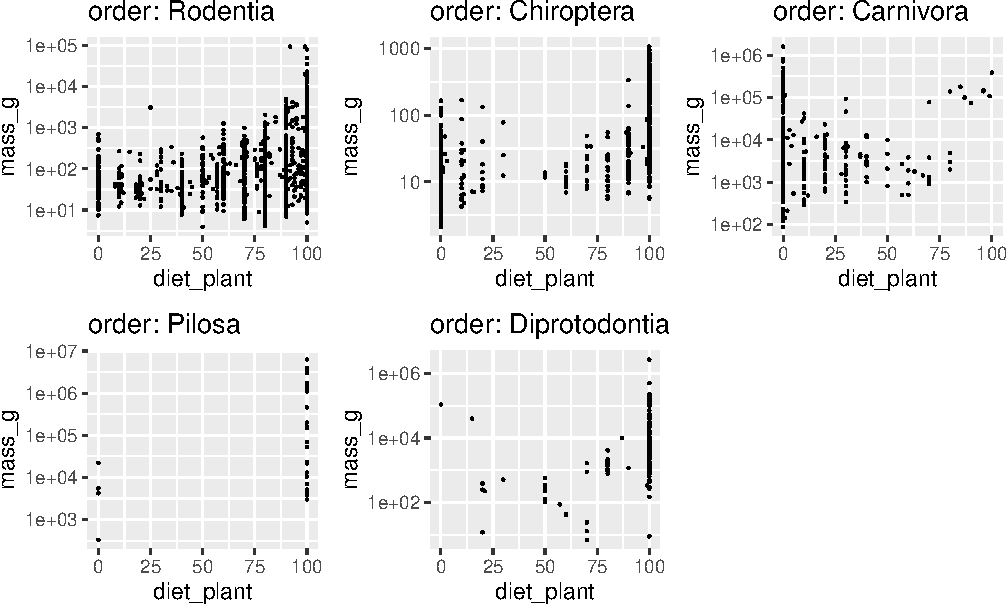
\includegraphics[width=\textwidth]{TRES-Tidy-Tutorial_files/figure-latex/unnamed-chunk-104-1} \end{center}

\end{document}
